% Generated by Sphinx.
\def\sphinxdocclass{report}
\documentclass[letterpaper,10pt,english]{sphinxmanual}
\usepackage[utf8]{inputenc}
\DeclareUnicodeCharacter{00A0}{\nobreakspace}
\usepackage[T1]{fontenc}
\usepackage{babel}
\usepackage{times}
\usepackage[Bjarne]{fncychap}
\usepackage{longtable}
\usepackage{sphinx}
\usepackage{multirow}


\title{PuppyIR Documentation}
\date{March 08, 2012}
\release{2.05}
\author{The PuppyIR Development Team}
\newcommand{\sphinxlogo}{}
\renewcommand{\releasename}{Release}
\makeindex

\makeatletter
\def\PYG@reset{\let\PYG@it=\relax \let\PYG@bf=\relax%
    \let\PYG@ul=\relax \let\PYG@tc=\relax%
    \let\PYG@bc=\relax \let\PYG@ff=\relax}
\def\PYG@tok#1{\csname PYG@tok@#1\endcsname}
\def\PYG@toks#1+{\ifx\relax#1\empty\else%
    \PYG@tok{#1}\expandafter\PYG@toks\fi}
\def\PYG@do#1{\PYG@bc{\PYG@tc{\PYG@ul{%
    \PYG@it{\PYG@bf{\PYG@ff{#1}}}}}}}
\def\PYG#1#2{\PYG@reset\PYG@toks#1+\relax+\PYG@do{#2}}

\def\PYG@tok@gd{\def\PYG@tc##1{\textcolor[rgb]{0.63,0.00,0.00}{##1}}}
\def\PYG@tok@gu{\let\PYG@bf=\textbf\def\PYG@tc##1{\textcolor[rgb]{0.50,0.00,0.50}{##1}}}
\def\PYG@tok@gt{\def\PYG@tc##1{\textcolor[rgb]{0.00,0.25,0.82}{##1}}}
\def\PYG@tok@gs{\let\PYG@bf=\textbf}
\def\PYG@tok@gr{\def\PYG@tc##1{\textcolor[rgb]{1.00,0.00,0.00}{##1}}}
\def\PYG@tok@cm{\let\PYG@it=\textit\def\PYG@tc##1{\textcolor[rgb]{0.25,0.50,0.56}{##1}}}
\def\PYG@tok@vg{\def\PYG@tc##1{\textcolor[rgb]{0.73,0.38,0.84}{##1}}}
\def\PYG@tok@m{\def\PYG@tc##1{\textcolor[rgb]{0.13,0.50,0.31}{##1}}}
\def\PYG@tok@mh{\def\PYG@tc##1{\textcolor[rgb]{0.13,0.50,0.31}{##1}}}
\def\PYG@tok@cs{\def\PYG@tc##1{\textcolor[rgb]{0.25,0.50,0.56}{##1}}\def\PYG@bc##1{\colorbox[rgb]{1.00,0.94,0.94}{##1}}}
\def\PYG@tok@ge{\let\PYG@it=\textit}
\def\PYG@tok@vc{\def\PYG@tc##1{\textcolor[rgb]{0.73,0.38,0.84}{##1}}}
\def\PYG@tok@il{\def\PYG@tc##1{\textcolor[rgb]{0.13,0.50,0.31}{##1}}}
\def\PYG@tok@go{\def\PYG@tc##1{\textcolor[rgb]{0.19,0.19,0.19}{##1}}}
\def\PYG@tok@cp{\def\PYG@tc##1{\textcolor[rgb]{0.00,0.44,0.13}{##1}}}
\def\PYG@tok@gi{\def\PYG@tc##1{\textcolor[rgb]{0.00,0.63,0.00}{##1}}}
\def\PYG@tok@gh{\let\PYG@bf=\textbf\def\PYG@tc##1{\textcolor[rgb]{0.00,0.00,0.50}{##1}}}
\def\PYG@tok@ni{\let\PYG@bf=\textbf\def\PYG@tc##1{\textcolor[rgb]{0.84,0.33,0.22}{##1}}}
\def\PYG@tok@nl{\let\PYG@bf=\textbf\def\PYG@tc##1{\textcolor[rgb]{0.00,0.13,0.44}{##1}}}
\def\PYG@tok@nn{\let\PYG@bf=\textbf\def\PYG@tc##1{\textcolor[rgb]{0.05,0.52,0.71}{##1}}}
\def\PYG@tok@no{\def\PYG@tc##1{\textcolor[rgb]{0.38,0.68,0.84}{##1}}}
\def\PYG@tok@na{\def\PYG@tc##1{\textcolor[rgb]{0.25,0.44,0.63}{##1}}}
\def\PYG@tok@nb{\def\PYG@tc##1{\textcolor[rgb]{0.00,0.44,0.13}{##1}}}
\def\PYG@tok@nc{\let\PYG@bf=\textbf\def\PYG@tc##1{\textcolor[rgb]{0.05,0.52,0.71}{##1}}}
\def\PYG@tok@nd{\let\PYG@bf=\textbf\def\PYG@tc##1{\textcolor[rgb]{0.33,0.33,0.33}{##1}}}
\def\PYG@tok@ne{\def\PYG@tc##1{\textcolor[rgb]{0.00,0.44,0.13}{##1}}}
\def\PYG@tok@nf{\def\PYG@tc##1{\textcolor[rgb]{0.02,0.16,0.49}{##1}}}
\def\PYG@tok@si{\let\PYG@it=\textit\def\PYG@tc##1{\textcolor[rgb]{0.44,0.63,0.82}{##1}}}
\def\PYG@tok@s2{\def\PYG@tc##1{\textcolor[rgb]{0.25,0.44,0.63}{##1}}}
\def\PYG@tok@vi{\def\PYG@tc##1{\textcolor[rgb]{0.73,0.38,0.84}{##1}}}
\def\PYG@tok@nt{\let\PYG@bf=\textbf\def\PYG@tc##1{\textcolor[rgb]{0.02,0.16,0.45}{##1}}}
\def\PYG@tok@nv{\def\PYG@tc##1{\textcolor[rgb]{0.73,0.38,0.84}{##1}}}
\def\PYG@tok@s1{\def\PYG@tc##1{\textcolor[rgb]{0.25,0.44,0.63}{##1}}}
\def\PYG@tok@gp{\let\PYG@bf=\textbf\def\PYG@tc##1{\textcolor[rgb]{0.78,0.36,0.04}{##1}}}
\def\PYG@tok@sh{\def\PYG@tc##1{\textcolor[rgb]{0.25,0.44,0.63}{##1}}}
\def\PYG@tok@ow{\let\PYG@bf=\textbf\def\PYG@tc##1{\textcolor[rgb]{0.00,0.44,0.13}{##1}}}
\def\PYG@tok@sx{\def\PYG@tc##1{\textcolor[rgb]{0.78,0.36,0.04}{##1}}}
\def\PYG@tok@bp{\def\PYG@tc##1{\textcolor[rgb]{0.00,0.44,0.13}{##1}}}
\def\PYG@tok@c1{\let\PYG@it=\textit\def\PYG@tc##1{\textcolor[rgb]{0.25,0.50,0.56}{##1}}}
\def\PYG@tok@kc{\let\PYG@bf=\textbf\def\PYG@tc##1{\textcolor[rgb]{0.00,0.44,0.13}{##1}}}
\def\PYG@tok@c{\let\PYG@it=\textit\def\PYG@tc##1{\textcolor[rgb]{0.25,0.50,0.56}{##1}}}
\def\PYG@tok@mf{\def\PYG@tc##1{\textcolor[rgb]{0.13,0.50,0.31}{##1}}}
\def\PYG@tok@err{\def\PYG@bc##1{\fcolorbox[rgb]{1.00,0.00,0.00}{1,1,1}{##1}}}
\def\PYG@tok@kd{\let\PYG@bf=\textbf\def\PYG@tc##1{\textcolor[rgb]{0.00,0.44,0.13}{##1}}}
\def\PYG@tok@ss{\def\PYG@tc##1{\textcolor[rgb]{0.32,0.47,0.09}{##1}}}
\def\PYG@tok@sr{\def\PYG@tc##1{\textcolor[rgb]{0.14,0.33,0.53}{##1}}}
\def\PYG@tok@mo{\def\PYG@tc##1{\textcolor[rgb]{0.13,0.50,0.31}{##1}}}
\def\PYG@tok@mi{\def\PYG@tc##1{\textcolor[rgb]{0.13,0.50,0.31}{##1}}}
\def\PYG@tok@kn{\let\PYG@bf=\textbf\def\PYG@tc##1{\textcolor[rgb]{0.00,0.44,0.13}{##1}}}
\def\PYG@tok@o{\def\PYG@tc##1{\textcolor[rgb]{0.40,0.40,0.40}{##1}}}
\def\PYG@tok@kr{\let\PYG@bf=\textbf\def\PYG@tc##1{\textcolor[rgb]{0.00,0.44,0.13}{##1}}}
\def\PYG@tok@s{\def\PYG@tc##1{\textcolor[rgb]{0.25,0.44,0.63}{##1}}}
\def\PYG@tok@kp{\def\PYG@tc##1{\textcolor[rgb]{0.00,0.44,0.13}{##1}}}
\def\PYG@tok@w{\def\PYG@tc##1{\textcolor[rgb]{0.73,0.73,0.73}{##1}}}
\def\PYG@tok@kt{\def\PYG@tc##1{\textcolor[rgb]{0.56,0.13,0.00}{##1}}}
\def\PYG@tok@sc{\def\PYG@tc##1{\textcolor[rgb]{0.25,0.44,0.63}{##1}}}
\def\PYG@tok@sb{\def\PYG@tc##1{\textcolor[rgb]{0.25,0.44,0.63}{##1}}}
\def\PYG@tok@k{\let\PYG@bf=\textbf\def\PYG@tc##1{\textcolor[rgb]{0.00,0.44,0.13}{##1}}}
\def\PYG@tok@se{\let\PYG@bf=\textbf\def\PYG@tc##1{\textcolor[rgb]{0.25,0.44,0.63}{##1}}}
\def\PYG@tok@sd{\let\PYG@it=\textit\def\PYG@tc##1{\textcolor[rgb]{0.25,0.44,0.63}{##1}}}

\def\PYGZbs{\char`\\}
\def\PYGZus{\char`\_}
\def\PYGZob{\char`\{}
\def\PYGZcb{\char`\}}
\def\PYGZca{\char`\^}
\def\PYGZsh{\char`\#}
\def\PYGZpc{\char`\%}
\def\PYGZdl{\char`\$}
\def\PYGZti{\char`\~}
% for compatibility with earlier versions
\def\PYGZat{@}
\def\PYGZlb{[}
\def\PYGZrb{]}
\makeatother

\begin{document}

\maketitle
\tableofcontents
\phantomsection\label{index::doc}


This documentation describes the PuppyIR project's open source, Python based, framework. This framework provides an open source environment for building information services, specifically for children, using a variety of tools, search engine wrappers, filters and more.

In order to best describe the framework and its uses, the documentation is split up into several sections:
\begin{itemize}
\item {} 
the \textbf{`about'} section, which details the design of the framework and how the various components relate to each other;

\item {} 
the \textbf{`using the framework'} section details various aspects pertaining to the usage of the framework;

\item {} 
the \textbf{`tutorials'} section, which provides practical examples of using the framework for a variety of audiences;

\item {} 
the \textbf{`extending'} section details how the framework can be extended to add new filters, modifiers and search engine wrappers;

\item {} 
the \textbf{`appendices'} section which details various supplementary materials that further expand on the other sections including an FAQ (frequently asked questions);

\item {} 
and, finally, the  \textbf{`API reference'} which details the components in framework (including details about their parameters etc).

\end{itemize}


\chapter{About the Framework}
\label{index:welcome-to-the-puppyir-framework-documentation}\label{index:about-the-framework}

\section{Overview and background of the PuppyIR Framework}
\label{overview:overview}\label{overview::doc}\label{overview:overview-and-background-of-the-puppyir-framework}
The framework is part of the PuppyIR project \footnote{
For more details about the PuppyIR project, please visit the project's website at: \href{http://www.puppyir.eu/}{http://www.puppyir.eu/}
}, funded by the European Union, which is investigating children's information retrieval (IR). The project's long term goal is to work towards universal access of information for both children and adults. As part of this, the framework is being developed as a suite of tools to assist developers and researchers in rapidly developing interaction IR applications for children.

In summary, it aims to:
\begin{enumerate}
\item {} 
Simplify the process of building interactive IR services;

\item {} 
provide a disparate and extensive suite of components, specifically tailored for children;

\item {} 
incorporate current research findings in children's IR;

\item {} 
be highly extensible (in all the main sections, and their respective components, of the framework), so that the framework can be adapted for an applications specific needs;

\item {} 
and, to provide extensive documentation {[}this document{]} with tutorials detailing how to use, extend and customise all the different parts of the framework.

\end{enumerate}


\subsection{The main features of the framework}
\label{overview:the-main-features-of-the-framework}
In this Chapter, the key functionalities of the framework are introduced and discussed; links are provided to the Chapters that provide more detailed commentary (and examples) of each functionality discussed here. To accomplish the aims listed above, the framework offers a developer, or researcher, a large variety of functionalities and associated components. These are split up into several distinct sections of the framework (for a full list, of all the individual components in these sections, please see consult the {\hyperref[api2.0:api]{\emph{PuppyIR API Reference}}}).


\subsubsection{Data Formatting}
\label{overview:data-formatting}
PuppyIR provides a standardised format for both queries and the results of a search, called a response. This is so that all the components are able to interoperate and also because having this consistency, makes it easier for developers/researchers to make use of these elements in their applications. This standardised format is an implementation of the \href{http://www.opensearch.org/Specifications/OpenSearch/1.1}{OpenSearch Standard} and the frameworks model of them can be found in PuppyIR's `query' and `response' classes; which are used by all the components that deal with such data. Many search services and API's support this standard, but, in some cases, some processing is required - in order to present data in a form that it is compliant with the OpenSearch standard (there are many examples of this processing in the framework's search engine wrappers).


\subsubsection{Architectural Paradigms}
\label{overview:architectural-paradigms}
There are two paradigms, included with the framework, for developers/researchers to use to build PuppyIR based applications, these are:
\begin{enumerate}
\item {} 
\textbf{One Pipeline, One Search Engine (Search Service)}: this is the standard (in terms of prototype and demonstrator adoption) paradigm for creating PuppyIR based applications. In it, a unique query and result pipeline is created for each search service. A search service is then linked to a source, i.e. a search engine wrapper like Bing or YouTube so that it can retrieve and process results. See: {\hyperref[service:service-architecture]{\emph{Paradigm 1 - One Pipeline, One Search Engine}}} for a more in-depth discussion of this paradigm.

\item {} 
\textbf{One Pipeline, Many Search Engines (Pipeline Service)}: an alternative to the search service paradigm, where only one query and result pipeline is created, various search engine wrappers can the be associated with the pipeline (defined by the pipeline service). Either search all, or search specific (i.e. search a specific search engine wrapper associated with the pipeline service) can be used to retrieve results using the defined query \& result pipelines. See: {\hyperref[pipeline:pipeline-architecture]{\emph{Paradigm 2 - One Pipeline, Many Search Engines}}} for a more in-depth discussion of this paradigm.

\end{enumerate}

A developer/researcher can select the paradigm that is most suited to their application; no matter which one is used, the same components and options (for configuring them) are available. This is due to all the components being generalised, in terms of their: interface, methods and parameters. All of the paradigms, however, make use of the `query' and `response' formats as mentioned earlier (however, the a pipeline service returns `response' objects in a slightly different way).


\subsubsection{Event and Query Logging}
\label{overview:event-and-query-logging}
Included with the framework are two kinds of logger, both of these are designed to assist developers and researchers in evaluating their applications, they are: (1) a query logger and (2), an event logger. Between these two kinds of logger, any kind of data required to be logged can be, for evaluation/analytical purposes.

Both the Search and Pipeline Services provide the ability to log queries, sent to the service in question, by a user. It is possible to log such queries at two distinct stages:
\begin{enumerate}
\item {} 
\textbf{Un-processed}: the query passed to the service in question before it goes through the query pipeline.

\item {} 
\textbf{Processed}: the query after it has gone through the pipeline (assuming it was not rejected during processing), for example it may have been extended via new terms being appended or spelling mistakes automatically being corrected.

\end{enumerate}

This allows two key areas to be investigated: (1) what sort of queries the users are sending and (2), the results of the query pipeline(s), defined in the application, on these queries.

The event logger provides a developer with a component that allows them to log only the details they wish (for the event being logged) to be logged for their specific application. This is possible via a keyword arguments parameter to the log method. However, an `identifier' and `type' must be supplied in order to differentiate the different events and assist with categorisation for analysis of the log file(s).


\subsubsection{Query and Result Filters}
\label{overview:query-and-result-filters}
Filters in both the Query and Result pipelines are components which decide whether or not to accept a specific result (in a response) or a query - depending upon which pipeline it belongs to.


\subsubsection{Query and Result Modifiers}
\label{overview:query-and-result-modifiers}

\subsubsection{Search Engine Wrappers}
\label{overview:search-engine-wrappers}

\subsubsection{Testing and Exception Handling}
\label{overview:testing-and-exception-handling}

\subsection{Extensibility of the framework}
\label{overview:extensibility-of-the-framework}
As stated in the aims detailed earlier, the extensibility of the framework and its components is a key aspect of its design. In is possible to add, customise and extend all of the components, discussed above, for use in a PuppyIR based application. However, several distinct areas have been selected to be written up for this document, i.e. the process for going about adding new components is detailed. These areas were identified as being the most likely for developers/researchers to wish to extend and are described briefly below.


\subsubsection{Search Engine Wrappers}
\label{overview:id2}
It is expected that the area, of the framework, especially, is one with great potential for future expansion and development. This is due to the inevitable influx of new API's and updates to the ones currently supported by the PuppyIR framework. The section detailing this area, therefore, looks at how to write new wrappers that are compatibly both with the architectural paradigms as well as the other components that interact with search engine wrappers (i.e. filters etc). See: {\hyperref[extendingSearchEngine:extending-the-search-engine]{\emph{Adding new Search Engine Wrappers}}} for more details on this.


\subsubsection{Query and Result Filters}
\label{overview:id3}

\subsubsection{Query and Result Modifiers}
\label{overview:id4}

\subsection{Other features and framework support}
\label{overview:other-features-and-framework-support}

\subsubsection{Which version of Python is the framework for?}
\label{overview:which-version-of-python-is-the-framework-for}
The PuppyIR framework is designed, built and maintained using Python 2.7; Python 3.x is not supported and earlier versions may have compatibility issue. It is, therefore, recommended to upgrade to Python 2.7 rather than using earlier versions. For details of some of the known Python compatibility issues please consult the {\hyperref[issues:issues]{\emph{Known issues with the PuppyIR framework}}} page.


\subsubsection{Standalone Services}
\label{overview:standalone-services}
The PuppyIR framework can be used to build a standalone service for research and development purposes.  This mode has minimal requirements and simplifies the process of building custom search services that do not require a user interface. See {\hyperref[standalone-service:building-a-standalone-puppyir-service]{\emph{Building a Standalone PuppyIR Service}}} for more information.


\subsubsection{Proxy Server Support}
\label{overview:proxy-server-support}
Many workplaces and research institutions use a proxy server and so, any applications created, using PuppyIR, would need to go through such a proxy server. The framework, therefore, offers a simple interface for its components that enables developers/researchers to easily set-up the components they are using to work with a defined proxy server. The code below shows how to create a service in both the paradigms, included with the framework:

\begin{Verbatim}[commandchars=\\\{\}]
\PYG{c}{\PYGZsh{} Set-up a config setting for a proxy server}
\PYG{n}{config} \PYG{o}{=} \PYG{p}{\PYGZob{}}\PYG{l+s}{"}\PYG{l+s}{proxyhost}\PYG{l+s}{"}\PYG{p}{:} \PYG{l+s}{"}\PYG{l+s}{http://your-proxy-server-address}\PYG{l+s}{"}\PYG{p}{\PYGZcb{}}

\PYG{c}{\PYGZsh{} -- Paradigm 1 and proxy servers --}
\PYG{c}{\PYGZsh{} ----------------------------------}

\PYG{c}{\PYGZsh{} Create a service manager and set it to use config}
\PYG{n}{sm} \PYG{o}{=} \PYG{n}{ServiceManager}\PYG{p}{(}\PYG{n}{config}\PYG{p}{)}

\PYG{c}{\PYGZsh{} Create a search service for Bing Web}
\PYG{n}{ss} \PYG{o}{=} \PYG{n}{SearchService}\PYG{p}{(}\PYG{n}{sm}\PYG{p}{,} \PYG{l+s}{"}\PYG{l+s}{bing\PYGZus{}web}\PYG{l+s}{"}\PYG{p}{)}

\PYG{c}{\PYGZsh{} Set our new search service to use the Bing wrapper}
\PYG{n}{ss}\PYG{o}{.}\PYG{n}{search\PYGZus{}engine} \PYG{o}{=} \PYG{n}{Bing}\PYG{p}{(}\PYG{n}{ss}\PYG{p}{)}

\PYG{c}{\PYGZsh{} Add new search service to ServiceManager}
\PYG{n}{sm}\PYG{o}{.}\PYG{n}{add\PYGZus{}search\PYGZus{}service}\PYG{p}{(}\PYG{n}{ss}\PYG{p}{)}

\PYG{c}{\PYGZsh{} -- Paradigm 2 and proxy servers --}
\PYG{c}{\PYGZsh{} ----------------------------------}

\PYG{c}{\PYGZsh{} Create a Pipeline Service called 'myPipeline' using config}
\PYG{n}{pipelineService} \PYG{o}{=} \PYG{n}{PipelineService}\PYG{p}{(}\PYG{n}{config}\PYG{p}{,} \PYG{l+s}{"}\PYG{l+s}{myPipeline}\PYG{l+s}{"}\PYG{p}{)}

\PYG{c}{\PYGZsh{} Create a Bing search engine wrapper}
\PYG{n}{bing} \PYG{o}{=} \PYG{n}{Bing}\PYG{p}{(}\PYG{n}{pipelineService}\PYG{p}{)}

\PYG{c}{\PYGZsh{} Add Bing to our search engine manager (this stores all our search engines)}
\PYG{n}{pipelineService}\PYG{o}{.}\PYG{n}{searchEngineManager}\PYG{o}{.}\PYG{n}{add\PYGZus{}search\PYGZus{}engine}\PYG{p}{(}\PYG{l+s}{"}\PYG{l+s}{Bing}\PYG{l+s}{"}\PYG{p}{,} \PYG{n}{bing}\PYG{p}{)}
\end{Verbatim}


\subsubsection{Django support}
\label{overview:django-support}
The PuppyIR framework can be integrated with the Django web application framework to provide a toolkit for rapidly prototyping and deploying search services for children on the web.  PuppyIR includes a number of components that augment the existing Django functionality. See {\hyperref[django-service:building-a-puppyir-django-service]{\emph{BaSe Tutorial: Building a PuppyIR/Django Service}}} for more information.

N.B. Django is provided as an example, the framework can also work with other Python based web application frameworks as no parts of the framework are tied into Django.


\section{Requirements and Installation}
\label{installation:requirements-and-installation}\label{installation::doc}\label{installation:id1}
The PuppyIR framework is Python-based and requires, in addition to Python itself, several external dependencies. It can either be installed as a standalone service, or combined with the Django web application framework to build web services. The requirements, both basic and those required for additional functionality, are detailed here.

Note: if you are running MacOS X, please ensure that you have \href{http://developer.apple.com/technologies/tools/}{X-Code} installed (either Version 3 or 4; this may be included on your install disc). This is required as several of the dependencies use X-Code's C compiler.


\subsection{PuppyIR and MacPorts}
\label{installation:puppyir-and-macports}
For developers using MacOS X, \href{http://www.macports.org/}{MacPorts} can be used to install all the PuppyIR framework requirements. If you wish to install these using MacPorts please ensure that you install the \emph{`py27'} versions. Please consult the MacPorts documentation for how to use MacPorts and then install all the basic and extra requirements (if required) using their port versions.

The one exception to the naming convention (of \emph{`py27'}) is setuptools, which has the Port name \textbf{`py-setuptools'}.


\subsection{Basic Requirements}
\label{installation:basic-requirements-label}\label{installation:basic-requirements}
The basic PuppyIR framework installation requires all of the following to be installed (in addition to the framework itself):
\begin{itemize}
\item {} 
\href{http://www.python.org/}{Python Programming Environment} (N.B. Python 3.x is not supported)

\item {} 
\href{http://pypi.python.org/pypi/setuptools}{Setuptools}

\item {} 
\href{http://code.google.com/p/feedparser/}{Universal Feed Parser}

\item {} 
\href{http://pypi.python.org/pypi/lxml/}{lxml}

\item {} 
\href{http://www.crummy.com/software/BeautifulSoup/\#Download}{BeautifulSoup}

\end{itemize}


\subsection{Extra Requirements}
\label{installation:extra-requirements-label}\label{installation:extra-requirements}
The following external dependencies are only required, if you intend to do any of the development tasks detailed below.

To create web services using the Django framework and/or to run the various prototypes and demonstrators:
\begin{itemize}
\item {} 
\href{https://www.djangoproject.com/}{Django Web Application Framework}

\end{itemize}

To run some of the prototype services included with the PuppyIR framework (specifically the JuSe prototype):
\begin{itemize}
\item {} 
\href{http://www.pythonware.com/products/pil/}{PIL (Python Imaging Library)}

\end{itemize}

If you require the use of the `spelling modifier' (see: {\hyperref[api2.0:puppy-spelling-mod]{\emph{SpellingModifier}}} for more on this component) install Enchant:
\begin{itemize}
\item {} 
\href{http://packages.python.org/pyenchant/}{Enchant}

\end{itemize}

If you require the use of a full text indexer:
\begin{itemize}
\item {} 
\href{http://pypi.python.org/pypi/Whoosh/\#downloads}{Whoosh}

\end{itemize}

If you wish to use the `SuitabilityFilter' \footnote{
For the `SuitabilityFilter' to work you need to have java added to your system path; how to go about this varies depending on the Operating System (OS) you are using - there are many articles on the internet explaining how to do this for all the major OS's so this is not detailed here.
} to filter results and/or make use of Strathclyde University's work in \textbf{`trunk/interfaces'} (see {\hyperref[repo:repo]{\emph{The structure and the PuppyIR repository}}} for more on the structure of the repository) you will need to install Java:
\begin{itemize}
\item {} 
\href{http://www.oracle.com/technetwork/java/javase/downloads/index.html}{Java}  - this site also contains installation instructions for Java.

\end{itemize}


\subsection{Basic Installation}
\label{installation:basic-installation}
The following sections provide instructions on installing each of the requirements, as detailed in {\hyperref[installation:basic-requirements-label]{\emph{Basic Requirements}}}.


\subsubsection{Install Python}
\label{installation:install-python}
If your system does not have Python installed, or you have an earlier version, you can find the latest 2.7 branch of Python \href{http://python.org/download/}{here}. Follow the installation instructions for your own operating system.

At present, Python 3.x is not supported and may cause problems if installed.  You can discover your current version of Python by launching a command prompt and typing the command `python'.  The version number should be displayed as shown below. If Python 3.0+ is installed, please install the earlier version (the 2.7 branch) to run PuppyIR.

\begin{Verbatim}[commandchars=\\\{\}]
\$ python
Python 2.7.1 (r271:86882M, Nov 30 2010, 10:35:34)
[GCC 4.2.1 (Apple Inc. build 5664)] on darwin
Type "help", "copyright", "credits" or "license" for more information.
\textgreater{}\textgreater{}\textgreater{}
\end{Verbatim}


\subsubsection{Install Setuptools}
\label{installation:install-setuptools}
This is a pre-requisite to allow several of the other basic dependencies to be installed.

Download the source from \href{http://pypi.python.org/pypi/setuptools}{http://pypi.python.org/pypi/setuptools}

\begin{Verbatim}[commandchars=\\\{\}]
\$ cd /path/to/source
\$ python setup.py install \# may require 'sudo'
\end{Verbatim}


\subsubsection{Install Universal Feed Parser}
\label{installation:install-universal-feed-parser}
This allows PuppyIR to parse RSS and Atom feeds.

Download the source from \href{http://code.google.com/p/feedparser/}{http://code.google.com/p/feedparser/}

\begin{Verbatim}[commandchars=\\\{\}]
\$ cd /path/to/source
\$ python setup.py install \# may require 'sudo'
\end{Verbatim}


\subsubsection{Install lxml}
\label{installation:install-lxml}
This allows PuppyIR to parse XML files.

Download the source from \href{http://pypi.python.org/pypi/lxml/}{http://pypi.python.org/pypi/lxml/}

\begin{Verbatim}[commandchars=\\\{\}]
\$ cd /path/to/source
\$ python setup.py install \# may require 'sudo'
\end{Verbatim}


\subsubsection{Install BeautifulSoup}
\label{installation:install-beautifulsoup}
This is a HTML/XML parser, one of its main functions is handling tree traversal automatically.

Download the source from \href{http://www.crummy.com/software/BeautifulSoup/\#Download}{http://www.crummy.com/software/BeautifulSoup/\#Download}

\begin{Verbatim}[commandchars=\\\{\}]
\$ cd /path/to/source
\$ python setup.py install \# may require 'sudo'
\end{Verbatim}


\subsubsection{Installing the PuppyIR Framework}
\label{installation:install-puppy-ir}\label{installation:installing-the-puppyir-framework}
There are two options for installing the PuppyIR framework itself, either you can install the latest development version, or, install a specific release of the framework.


\subsubsection{Option 1: Installing a specific release}
\label{installation:option-1-installing-a-specific-release}
If you require a specific release, for your application, or simply wish to use a release that is likely to be stable, then choose this option and follow the instructions below.

Download the specific release you want from \href{http://sourceforge.net/projects/puppyir/files/release/}{http://sourceforge.net/projects/puppyir/files/release/} then:

\begin{Verbatim}[commandchars=\\\{\}]
\$ cd path/to/puppyir
\$ python setup.py install \# may require 'sudo'
\end{Verbatim}


\subsubsection{Option 2: Installing the development version}
\label{installation:option-2-installing-the-development-version}
Alternatively, the very latest release - the development version - can be checked out of the repository by following the instructions below:

\begin{Verbatim}[commandchars=\\\{\}]
\$ svn export https://puppyir.svn.sourceforge.net/svnroot/puppyir/trunk/framework puppyir
\$ cd puppyir
\$ python setup.py install \# may require 'sudo'
\end{Verbatim}

N.B. the development version is not guaranteed to be stable and may be incompatible with certain prototypes and/or demonstrators.


\subsection{Installing the Extras}
\label{installation:installing-the-extras}
The following sections, provide instructions on installing each of the extra requirements (as detailed in {\hyperref[installation:extra-requirements-label]{\emph{Extra Requirements}}}).


\subsubsection{Install Django}
\label{installation:install-django}
(Only required if building web services that require or make use of the Django web application framework)

Django is a Python based web framework designed to build web applications quickly, installing this allows developers/researchers to take advantage of the many features offered by Django and also to run the prototypes and demonstrators bundled with the framework.

Download source from \href{https://www.djangoproject.com/download/}{https://www.djangoproject.com/download/}

\begin{Verbatim}[commandchars=\\\{\}]
\$ cd /path/to/source
\$ python setup.py install \# may require 'sudo'
\end{Verbatim}


\subsubsection{Install Python Imaging Library (PIL)}
\label{installation:install-python-imaging-library-pil}
(Only required for the JuSe prototype)

This is a library that provides allows various image processing tasks to be done on a large variety of image formats.

Download the source from \href{http://www.pythonware.com/products/pil/}{http://www.pythonware.com/products/pil/}

\begin{Verbatim}[commandchars=\\\{\}]
\$ cd /path/to/source
\$ python setup.py install \# may require 'sudo'
\end{Verbatim}


\subsubsection{Install Enchant}
\label{installation:install-enchant}
(Only required if using the `spelling modifier' - see: {\hyperref[api2.0:puppy-spelling-mod]{\emph{SpellingModifier}}} for more on this component)

This is a library that checks the spelling of words and provides a list of suggested correct spellings.

It requires enchant library (version 1.5.0 or greater) which can be downloaded at \href{http://www.abisource.com/projects/enchant/}{http://www.abisource.com/projects/enchant/} - installation instructions can be found on this site as well.

Then download Enchant for Python from \href{http://packages.python.org/pyenchant/}{http://packages.python.org/pyenchant/}

\begin{Verbatim}[commandchars=\\\{\}]
\$ cd /path/to/source
\$ python setup.py install \# may require 'sudo'
\end{Verbatim}


\subsubsection{Install Whoosh}
\label{installation:install-whoosh}
(Only required for local full text indexing and to run certain prototypes \& demonstrators)

Download source from \href{http://pypi.python.org/pypi/Whoosh/\#downloads}{http://pypi.python.org/pypi/Whoosh/\#downloads}

\begin{Verbatim}[commandchars=\\\{\}]
\$ cd /path/to/source
\$ python setup.py install \# may require 'sudo'
\end{Verbatim}


\section{Paradigm 1 - One Pipeline, One Search Engine}
\label{service:service-architecture}\label{service::doc}\label{service:paradigm-1-one-pipeline-one-search-engine}
The core component of a PuppyIR based application is a search service in this paradigm. A search service contains a variety of individual components that, when combined together, allow for: searching , retrieving and processing the results - from a specific defined search engine. These search services are stored and managed by a service manager. The diagram below shows the structure of a search service from its owner, the service manager, to all the individual components contained within the search service.
\begin{figure}[htbp]
\centering
\capstart

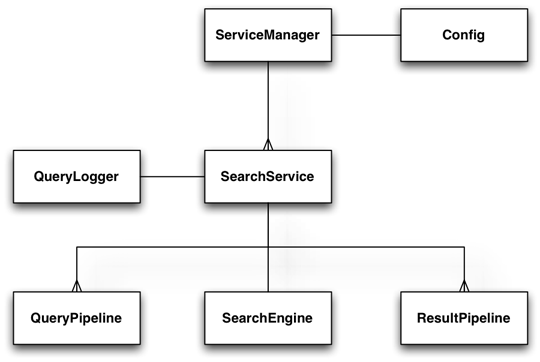
\includegraphics{puppy-service-architecture.png}
\caption{\emph{The basic architecture of a PuppyIR application, using the `Search Service' paradigm.}}\end{figure}


\subsection{Description of the components}
\label{service:description-of-the-components}
The roles of the components are as follows:
\begin{itemize}
\item {} 
\textbf{Service Manager}: this is in charge of managing (adding and deleting) all the search services used by an application.

\item {} 
\textbf{Config}: local configuration options (e.g. for proxies, API keys and log files).

\item {} 
\textbf{Search Service}: a single search service, with its own query logger and distinct query \& result pipelines.

\item {} 
\textbf{Query Logger}: logs queries, sent to a search service, to file (available for both un-processed and processed query logging - more on this later).

\item {} 
\textbf{Search Engine}:  this is the search engine wrapper for a specific `search service' - e.g. a `search service' that uses the YouTube search engine (wrapper).

\item {} 
\textbf{Query Pipeline}: a collection of query filters and modifiers associated with a specific `search service'.

\item {} 
\textbf{Result Pipeline}: a collection of result filters and modifiers associated with a specific `search service'.

\end{itemize}


\subsection{Data flow in the `Service' paradigm}
\label{service:data-flow-in-the-service-paradigm}
The diagram below shows the basic flow between a user issuing a query and their results being returned.
\begin{figure}[htbp]
\centering
\capstart

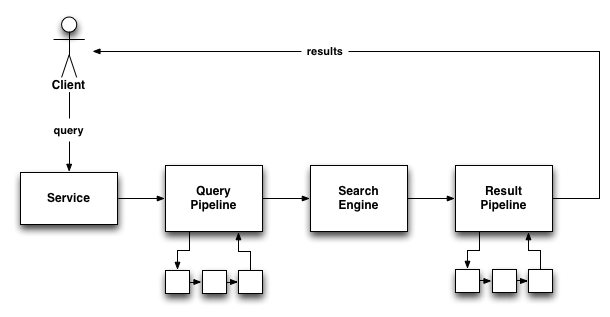
\includegraphics{puppy-pipelines.png}
\caption{\emph{The basic data-flow in the `Search Service' paradigm.}}\end{figure}

The `search service' is passed a query, by the user/client, via the search method in the `search service' (simple search is also available; this skips the query and result pipelines). It then goes through the query pipeline, first running all the query filters and then all the query modifiers. The processed query is then passed to the `search engine' (defined for the current `search service') and the results retrieved using the search method contained in the `search engine' wrapper. The results are then passed through the result pipeline, first by running all the result filters and then, finally, all the result modifiers. Following the completion of the `result pipeline', the processed results are then returned to the user/client.


\subsection{On Filters, Modifiers and Query Logging}
\label{service:on-filters-modifiers-and-query-logging}
Within each of these pipelines (query and result) there are both filters and modifiers. Filters are executed first and then, following this, the modifiers are executed.

The distinction between a filter and a modifier is as follows:
\begin{itemize}
\item {} 
\textbf{Filters}: these reject or accept a query, or result, based on a defined criteria. For example a blacklist filter rejects queries containing one or more blacklisted words.

\item {} 
\textbf{Modifiers}: these change the content of a query, or result, based on a defined behaviour. For example, appending “for kids” to every query.

\end{itemize}

There are two points at which queries can be logged: before the query goes through the query pipeline and after (i.e. un-processed and processed). The default is to log queries before processing - if a query logger has been added. The code below shows how to add a query logger and set it so that processed queries are logged, in addition to un-processed ones:

\begin{Verbatim}[commandchars=\\\{\}]
\PYG{k+kn}{from} \PYG{n+nn}{puppy.logging} \PYG{k+kn}{import} \PYG{n}{QueryLogger}
\PYG{k+kn}{from} \PYG{n+nn}{puppy.service} \PYG{k+kn}{import} \PYG{n}{ServiceManager}\PYG{p}{,} \PYG{n}{SearchService}

\PYG{n}{config} \PYG{o}{=} \PYG{p}{\PYGZob{}}\PYG{l+s}{"}\PYG{l+s}{log\PYGZus{}dir}\PYG{l+s}{"}\PYG{p}{:} \PYG{l+s}{"}\PYG{l+s}{/path/to/log/dir}\PYG{l+s}{"}\PYG{p}{\PYGZcb{}} \PYG{c}{\PYGZsh{} Sets the log directory}
\PYG{n}{sm} \PYG{o}{=} \PYG{n}{ServiceManager}\PYG{p}{(}\PYG{n}{config}\PYG{p}{)}
\PYG{n}{ss} \PYG{o}{=} \PYG{n}{SearchService}\PYG{p}{(}\PYG{n}{sm}\PYG{p}{,} \PYG{l+s}{"}\PYG{l+s}{bing\PYGZus{}web}\PYG{l+s}{"}\PYG{p}{)}
\PYG{n}{sm}\PYG{o}{.}\PYG{n}{add\PYGZus{}search\PYGZus{}service}\PYG{p}{(}\PYG{n}{ss}\PYG{p}{)}
\PYG{n}{ss}\PYG{o}{.}\PYG{n}{search\PYGZus{}engine} \PYG{o}{=} \PYG{n}{Bing}\PYG{p}{(}\PYG{n}{ss}\PYG{p}{)}

\PYG{c}{\PYGZsh{} Assign QueryLogger to SearchService}
\PYG{n}{ss}\PYG{o}{.}\PYG{n}{query\PYGZus{}logger} \PYG{o}{=} \PYG{n}{QueryLogger}\PYG{p}{(}\PYG{n}{ss}\PYG{p}{)}
\PYG{n}{ss}\PYG{o}{.}\PYG{n}{postLogging} \PYG{o}{=} \PYG{n+nb+bp}{True} \PYG{c}{\PYGZsh{} Activate post-pipeline query logging}
\end{Verbatim}


\subsection{The Query and Results formats}
\label{service:the-query-and-results-formats}
Referring to the data flow diagram above, the formats of a query and results are as follows:
\begin{itemize}
\item {} 
A query is in the `Query' format (for more see: {\hyperref[api2.0:puppy-query]{\emph{Query}}}).

\item {} 
The results are in the `Response' format (for more see: {\hyperref[api2.0:puppy-response]{\emph{Response}}}); this is what is returned by the search call (for the search engine in question).

\end{itemize}

Both the Query and Response formats are implementations of the OpenSearch specification; for more details, see the links below:
\begin{itemize}
\item {} 
\href{http://www.opensearch.org/Specifications/OpenSearch/1.1\#OpenSearch\_Query\_element}{OpenSearch Query}.

\item {} 
\href{http://www.opensearch.org/Specifications/OpenSearch/1.1\#OpenSearch\_response\_elements}{OpenSearch Response}.

\end{itemize}


\section{Paradigm 2 - One Pipeline, Many Search Engines}
\label{pipeline:paradigm-2-one-pipeline-many-search-engines}\label{pipeline::doc}\label{pipeline:pipeline-architecture}
The core idea behind this alternate paradigm is that you create and manage one pipeline - to which search engines can then be added. This is in contrast to the ‘search service’ paradigm ({\hyperref[service:service-architecture]{\emph{Paradigm 1 - One Pipeline, One Search Engine}}}), where each search service, and its associated search engine wrapper, has its own distinct pipeline. Like with the ‘Search Service’ paradigm, there is a query pipeline and the result pipeline, but, in addition to this, there is an additional pipeline: the search engine pipeline (which makes use of a search engine manager; this is equivalent, in most respects, to the ‘Search Service Manager’ from the ‘search service’ paradigm).

The picture below shows how all these components relate to each other:
\begin{figure}[htbp]
\centering
\capstart

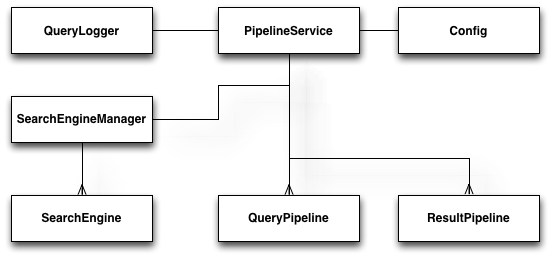
\includegraphics{puppy-pipeline-architecture.png}
\caption{\emph{The basic architecture of a PuppyIR application, using the `Pipeline Service' paradigm.}}\end{figure}


\subsection{Description of the components}
\label{pipeline:description-of-the-components}
Each of the key components, shown in the picture above, are summarised (in terms of how they relate to this paradigm) below; except for the ‘Query Logger’ and ‘Config’ components as these are identical to those found in the ‘Search Service’ architecture.

The roles of the components are as follows:
\begin{itemize}
\item {} 
\textbf{Pipeline Service}: this is the main component in this paradigm as it is in charge of managing and running the pipeline it defines (i.e. all the filters and modifiers). It also contains the next key component, the `search engine manager'.

\item {} 
\textbf{Search Engine Manager}: this component is, roughly, equivalent to the `search service manager' as found in the ‘search service’ paradigm; except that it manages search engines as opposed to search services. Its main tasks are adding and removing search engines.

\item {} 
\textbf{Search Engine}: this is the component managed by the search engine manager and is the same as in the ‘search service’ paradigm; except that it’s linked to the `pipeline service' not a search service. Like in ‘search service’ each search engine has a name assigned to it and the `search engine manager' looks for, deletes and retrieves search engines using this variable.

\item {} 
\textbf{Query and Result Pipelines}: these are exactly the same as their counterparts in the ‘search service’ paradigm, excepting that they are stored by a `pipeline service'.

\end{itemize}


\subsection{Data flow in the `Pipeline' paradigm}
\label{pipeline:data-flow-in-the-pipeline-paradigm}
The data flow in this paradigm is a little more complicated than in the ‘search service’ paradigm, due to the extra complexity introduced by having multiple search engines associated with one pipeline. The picture below shows the data flow between a user issuing a query and their receiving the result(s) of this query.
\begin{figure}[htbp]
\centering
\capstart

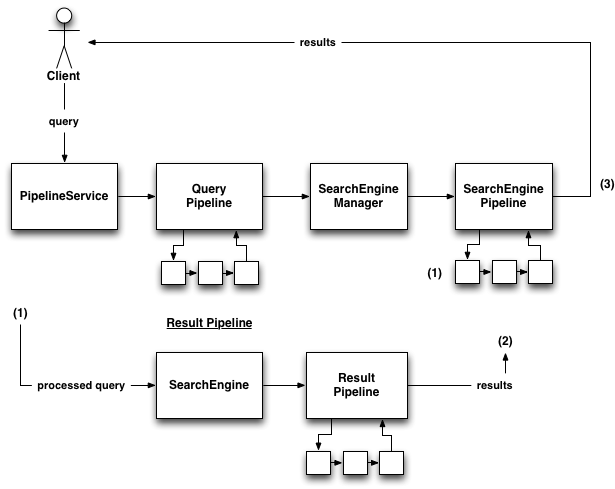
\includegraphics{puppy-pipeline-data-flow.png}
\caption{\emph{The basic data-flow diagram for the `Pipeline Service' paradigm.}}\end{figure}

The `pipeline service' is passed a query, by the user/client, via one of two methods: search all or search specific. From here, the query pipeline is run (once; even if there are multiple search engines - since they all have the same query and query pipeline), first going through all the filters and then all the modifiers. Following this, the `search engine manager' is called to retrieve either: all the search engines it manages, or one specific one. The next step is to run through the `search engine pipeline' with the results of the previous step. (1) shows the entry point for this process, at this stage either each search engine will be processed in turn or, in the case of a specific search, only one will be processed (as defined by the search specific call).

In the above diagram, the section under the label `Result Pipeline' shows how the processing of a search engine works:
\begin{itemize}
\item {} 
the processed query is passed to the current search engine (going through the pipeline);

\item {} 
next, the search method for this search engine is called and the results retrieved;

\item {} 
then the result filters, followed by the result modifiers are run (this step is the same as the result pipeline from `search service' - just applied to each search engine in turn);

\item {} 
lastly, the results from the current search engine are added to the overall `results' at (2).

\end{itemize}

Once the above process has been completed, for each search engine, the overall `results' are returned - (3) shows the point at which the overall `results' are complete and can then be returned to the user/client.


\subsection{On Filters, Modifiers and Query Logging}
\label{pipeline:on-filters-modifiers-and-query-logging}
Within the query and result pipelines there are both filters and modifiers. Filters are executed first and then, following this, the modifiers are executed.

The distinction between a filter and a modifier is as follows:
\begin{itemize}
\item {} 
\textbf{Filters}: these reject or accept a query, or result, based on a defined criteria. For example a blacklist filter rejects queries containing one or more blacklisted words.

\item {} 
\textbf{Modifiers}: these change the content of a query, or result, based on a defined behaviour. For example, appending “for kids” to every query.

\end{itemize}

There are many different filters and modifiers available for both of these pipelines, please consult the {\hyperref[api2.0:api]{\emph{PuppyIR API Reference}}} page for details of what is available.

There are two points at which queries can be logged: before the query goes through the query pipeline and after; i.e. un-processed and processed. The default is to log queries before processing - if a query logger has been added. The code below shows how to add a query logger and set it so that processed queries are logged, in addition to un-processed ones:

\begin{Verbatim}[commandchars=\\\{\}]
\PYG{k+kn}{from} \PYG{n+nn}{puppy.logging} \PYG{k+kn}{import} \PYG{n}{QueryLogger}
\PYG{k+kn}{from} \PYG{n+nn}{puppy.pipeline} \PYG{k+kn}{import} \PYG{n}{PipelineService}

\PYG{n}{config} \PYG{o}{=} \PYG{p}{\PYGZob{}}\PYG{l+s}{"}\PYG{l+s}{log\PYGZus{}dir}\PYG{l+s}{"}\PYG{p}{:} \PYG{l+s}{"}\PYG{l+s}{/path/to/log/dir}\PYG{l+s}{"}\PYG{p}{\PYGZcb{}} \PYG{c}{\PYGZsh{} Sets the log directory}
\PYG{n}{pm} \PYG{o}{=} \PYG{n}{PipelineService}\PYG{p}{(}\PYG{n}{config}\PYG{p}{)}
\PYG{n}{pm}\PYG{o}{.}\PYG{n}{query\PYGZus{}logger} \PYG{o}{=} \PYG{n}{QueryLogger}\PYG{p}{(}\PYG{n}{pm}\PYG{p}{)}
\PYG{n}{pm}\PYG{o}{.}\PYG{n}{postLogging} \PYG{o}{=} \PYG{n+nb+bp}{True} \PYG{c}{\PYGZsh{} Activate post-pipeline query logging}
\end{Verbatim}


\subsection{The Query and Results formats}
\label{pipeline:the-query-and-results-formats}
Referring to the data flow diagram above, the formats of a query and results are:
\begin{itemize}
\item {} 
A query is in the `Query' format (for more see: {\hyperref[api2.0:puppy-query]{\emph{Query}}}).

\item {} 
The results format is a Python dictionary, with one entry for each search engine; the key being the named assigned to the search engine and the value being the response (for more see: {\hyperref[api2.0:puppy-response]{\emph{Response}}}) object returned from the search call (for the search engine in question).

\end{itemize}

Both the Query and Response formats are implementations of the OpenSearch specification; for more details, see the links below:
\begin{itemize}
\item {} 
\href{http://www.opensearch.org/Specifications/OpenSearch/1.1\#OpenSearch\_Query\_element}{OpenSearch Query}.

\item {} 
\href{http://www.opensearch.org/Specifications/OpenSearch/1.1\#OpenSearch\_response\_elements}{OpenSearch Response}.

\end{itemize}


\subsection{Possible advantages of using this architecture}
\label{pipeline:possible-advantages-of-using-this-architecture}
This paradigm has the potential to be more efficient than the ‘search service’ paradigm, in terms of code and effort on the part of a developer/researcher, in the following ways:
\begin{itemize}
\item {} 
If you want the same pipeline (filters etc) for multiple services you only need to set the pipeline up once and can just add the search engines you want to the `search engine manager' (contained by your `pipeline service').

\item {} 
Related to the above point, is that the Query pipeline is only run once with `searchAll' because all the search engines use the same pipeline.

\item {} 
Less code for getting results - just a simple `searchAll' call rather than a search call for each search service and the associated code to handle this.

\end{itemize}


\subsection{Further Reading}
\label{pipeline:further-reading}
An example of the usage of this paradigm is given in: {\hyperref[pipeline-tutorial:pipeline-puppyir-tutorial]{\emph{Pipeline Tutorial: DeeSe (Detective Search)}}}.


\chapter{Using the Framework}
\label{index:using-the-framework}

\section{Running Prototypes}
\label{prototypes::doc}\label{prototypes:running-prototypes}\label{prototypes:prototypes}
Several prototype services are available as examples of how children's information services can built using the framework.
\begin{itemize}
\item {} 
\textbf{aMuSeV2}: a child friendly Multimedia Search engine mash-up search service allowing YouTube, Bing Image and Picassa to be searched for videos and images.

\item {} 
\textbf{aMuSeV3}: a child friendly search service allowing for the retrieving of video \& image search results and the exploration of these results via the generation of new queries.

\item {} 
\textbf{BaSe}: Basic Search - a bare bones search service with no frills.

\item {} 
\textbf{IfSe}: Information Foraging Search - an application created as a tutorial (see: {\hyperref[ifse-tutorial:information-foraging-puppyir-tutorial]{\emph{IfSe Tutorial: Information Foraging Search Application}}}) for using the PuppyIR framework to create a pipeline.

\item {} 
\textbf{MaSe}: Multimedia Search Engine Mash-up: an application created as a tutorial (see: {\hyperref[mase-tutorial:mase-mash-up-search-engine-puppyir-tutorial]{\emph{MaSe Tutorial: Mash-up Search Engine Application}}}) for using PuppyIR to create a customisable web application and in doing so, introduce web programming to school children.

\item {} 
\textbf{SeSu}: Search and Suggest - a search service which filters results by their suitability for children as well as providing search suggestions for new queries.

\end{itemize}


\subsection{Downloading the Prototypes}
\label{prototypes:downloading-the-prototypes}
All the prototypes require Django to be installed to use them. If you do not have Django installed, then please visit the {\hyperref[installation:requirements-and-installation]{\emph{Requirements and Installation}}} page and install them before downloading the prototypes.

In addition, IfSe and MaSe also require Whoosh to be installed to use them, if you do not have Whoosh installed please visit the installation page, as detailed above, and install Whoosh.

The source code for all the prototype services can then be downloaded as follows:

\begin{Verbatim}[commandchars=\\\{\}]
\$ svn co https://puppyir.svn.sourceforge.net/svnroot/puppyir/trunk/prototypes prototypes
\end{Verbatim}

To download a specific prototype, use the command as follows substituting in the name of the application (in this case, you will need to amend the paths to run the prototypes by removing the `prototypes' part of the path as noted in the \textbf{run} sections of this page):

\begin{Verbatim}[commandchars=\\\{\}]
\$ svn co https://puppyir.svn.sourceforge.net/svnroot/puppyir/trunk/prototypes/\textless{}APPNAME\textgreater{} \textless{}APPNAME\textgreater{}
\end{Verbatim}


\subsection{Using aMuSeV2: a Multimedia Search engine mash-up}
\label{prototypes:using-amusev2-a-multimedia-search-engine-mash-up}
aMuSeV2 allows video and picture results to be retrieved from YouTube, Bing and Picassa. The results are then scaled according to relevance; all results are draggable allowing them to be arranged as the user wishes.
\begin{figure}[htbp]
\centering
\capstart

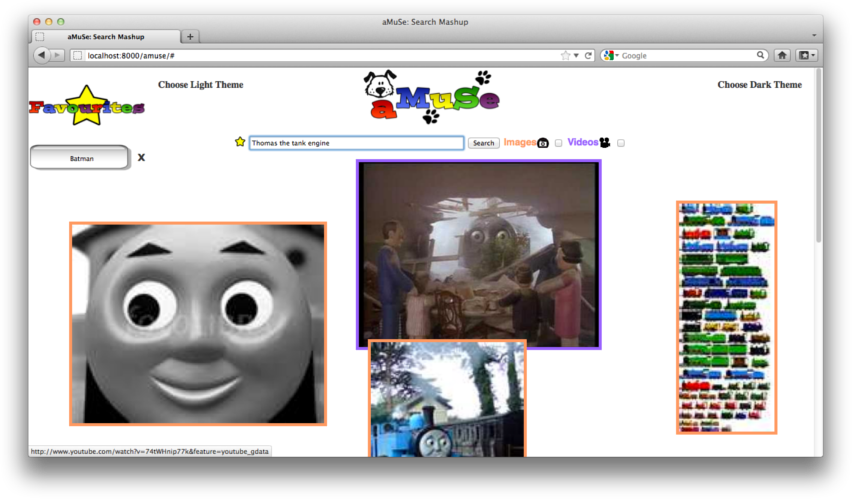
\includegraphics{puppy-amuse.png}
\caption{\emph{aMuSeV2 showing a video/image collage of `Thomas the Tank Engine' results.}}\end{figure}


\subsubsection{Run aMuSeV2}
\label{prototypes:run-amusev2}
\begin{Verbatim}[commandchars=\\\{\}]
\$ cd /path/to/prototypes/amuseV2
\$ python manage.py runserver
\end{Verbatim}

Visit: \href{http://localhost:8000/amuse}{http://localhost:8000/amuse}


\subsection{Using aMuSeV3: a Multimedia Search engine mash-up and browsing application}
\label{prototypes:using-amusev3-a-multimedia-search-engine-mash-up-and-browsing-application}
aMuSeV3 allows video and picture results to be retrieved from YouTube and Bing image search. The results are then, randomly (albeit, with a left-right-top-bottom approximation of relevance), arranged in a collage of images and videos. Videos can be played in-line; clicking on an image will generate a new query which will return a new collage of results.

aMuSeV3 is only compatible with Python Version 2.7 - if you have an earlier version then please install Python 2.7 to use this prototype.
\begin{figure}[htbp]
\centering
\capstart

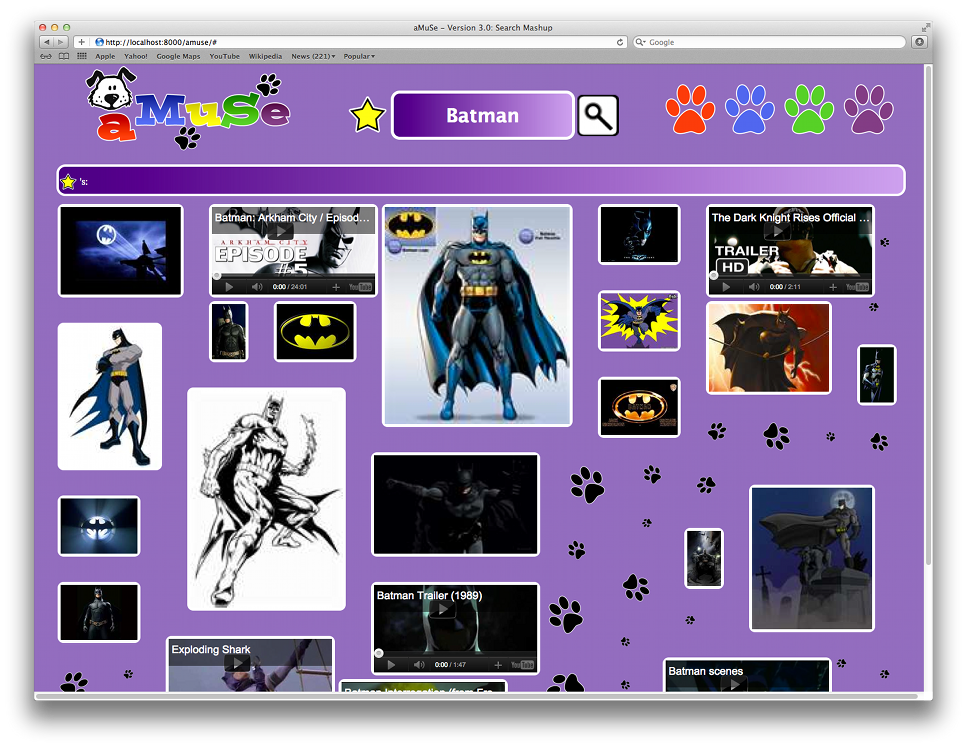
\includegraphics{puppy-amuseV3.png}
\caption{\emph{aMuSeV3 showing a video/image collage of `Batman' results.}}\end{figure}


\subsubsection{Run aMuSeV3}
\label{prototypes:run-amusev3}
\begin{Verbatim}[commandchars=\\\{\}]
\$ cd /path/to/prototypes/amuseV3
\$ python manage.py runserver
\end{Verbatim}

Visit: \href{http://localhost:8000/amuse}{http://localhost:8000/amuse}


\subsection{Using BaSe: Basic Search}
\label{prototypes:using-base-basic-search}
This is a simple `google-like' interface to illustrate a simple search interface.
\begin{figure}[htbp]
\centering
\capstart

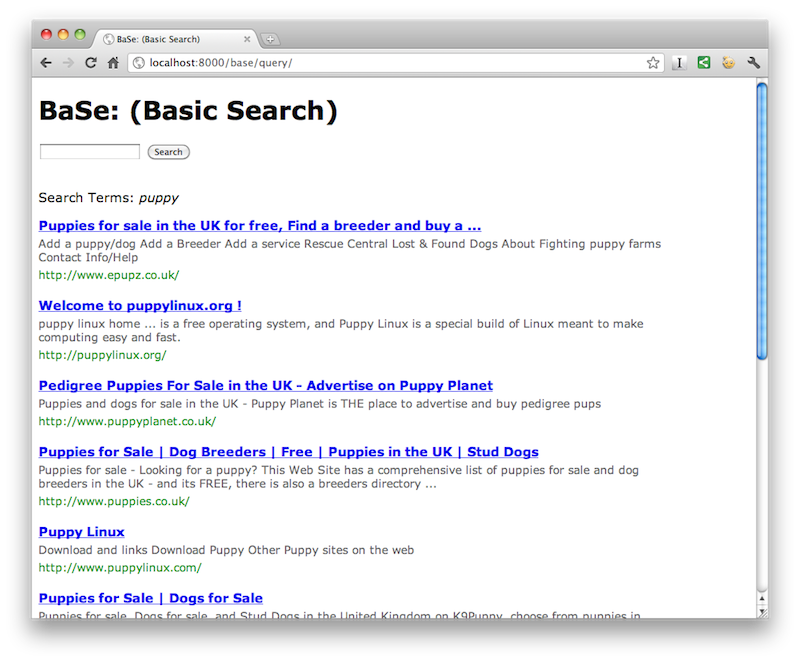
\includegraphics{puppy-base.png}
\caption{\emph{BaSe running on a local machine showing web results for the query `puppy'.}}\end{figure}


\subsubsection{Run BaSe}
\label{prototypes:run-base}
\begin{Verbatim}[commandchars=\\\{\}]
\$ cd /path/to/prototypes/base-tutorial
\$ python manage.py runserver
\end{Verbatim}

Visit: \href{http://localhost:8000/base}{http://localhost:8000/base}


\subsection{Using IfSe: Information Foraging Search}
\label{prototypes:using-ifse-information-foraging-search}
This prototype is part of a tutorial (see: {\hyperref[ifse-tutorial:information-foraging-puppyir-tutorial]{\emph{IfSe Tutorial: Information Foraging Search Application}}}) that teaches how to go about retrieving results from search engine wrappers, logging queries, generating suggestions and how to filter queries.
\begin{figure}[htbp]
\centering
\capstart

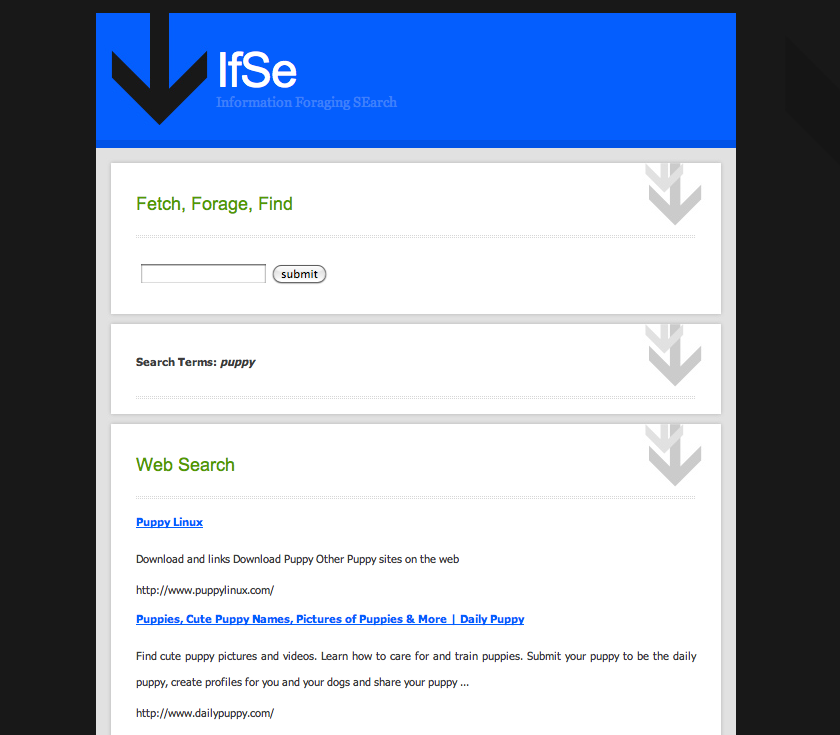
\includegraphics{puppy-ifse-before.png}
\caption{\emph{IfSe running on a local machine showing web results for the query `puppy'.}}\end{figure}


\subsubsection{Run IfSe}
\label{prototypes:run-ifse}
\begin{Verbatim}[commandchars=\\\{\}]
\$ cd /path/to/prototypes/ifse-tutorial
\$ python manage.py runserver
\end{Verbatim}

Visit: \href{http://localhost:8000/ifse}{http://localhost:8000/ifse}


\subsection{Using MaSe: Multimedia Mash-up Search Engine}
\label{prototypes:using-mase-multimedia-mash-up-search-engine}
MaSe is an application designed to allow children to create and customise their own search engine - retrieving results from a variety of sources and formats. See the MaSe tutorial for more details about the application {\hyperref[mase-tutorial:mase-mash-up-search-engine-puppyir-tutorial]{\emph{MaSe Tutorial: Mash-up Search Engine Application}}}.
\begin{figure}[htbp]
\centering
\capstart

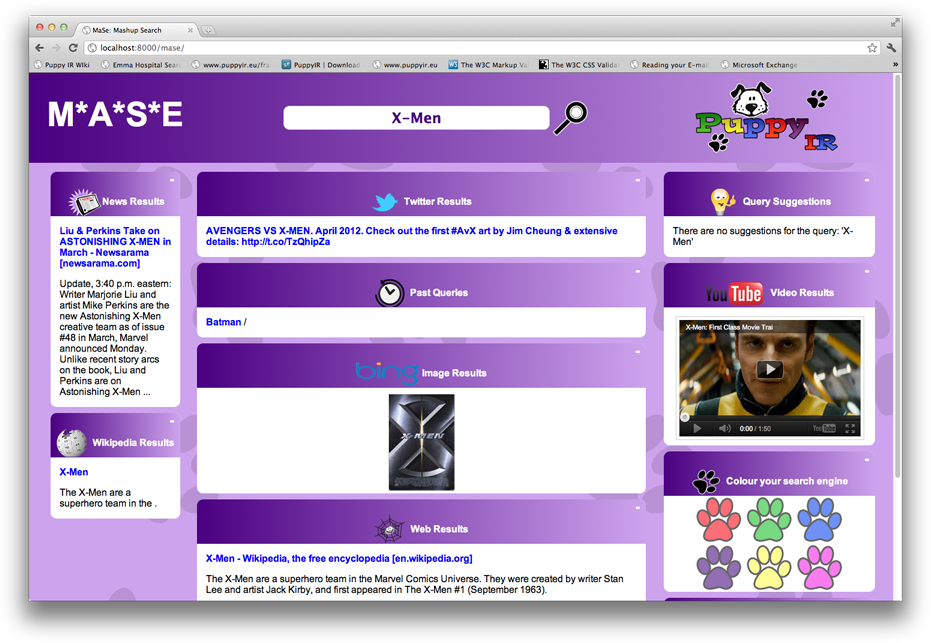
\includegraphics{mase-7-all.png}
\caption{\emph{MaSe running on a local machine showing web results for the query `X-Men'.}}\end{figure}


\subsubsection{Run MaSe}
\label{prototypes:run-mase}
\begin{Verbatim}[commandchars=\\\{\}]
\$ cd /path/to/prototypes/mase-tutorial
\$ python manage.py runserver
\end{Verbatim}

Visit: \href{http://localhost:8000/mase}{http://localhost:8000/mase}


\subsection{Using SeSu: Search and Suggest}
\label{prototypes:using-sesu-search-and-suggest}
SeSu is a prototype service that investigates query suggestions and suitability filters for children's web search.
\begin{figure}[htbp]
\centering
\capstart

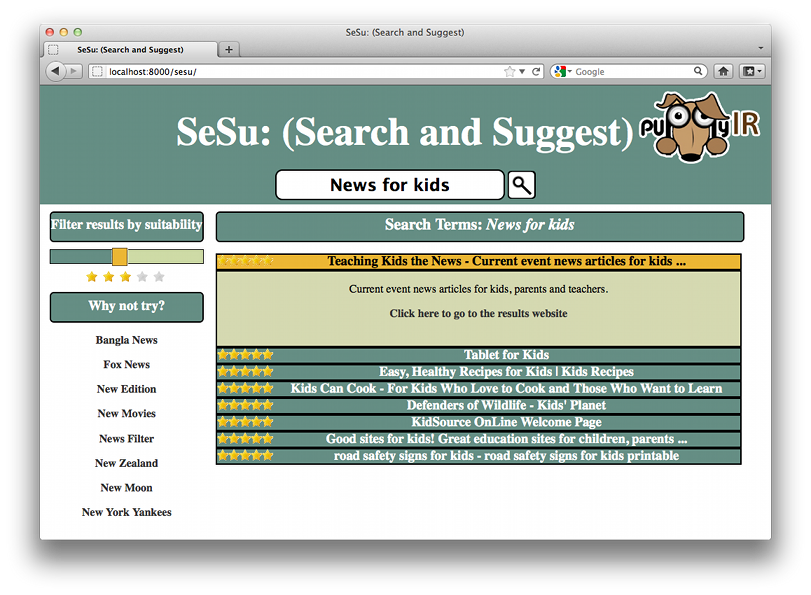
\includegraphics{puppy-sesu.png}
\caption{\emph{SeSu showing results, with their suitability rating, for a query about the news.}}\end{figure}


\subsubsection{Run SeSu}
\label{prototypes:run-sesu}
\begin{Verbatim}[commandchars=\\\{\}]
\$ cd /path/to/prototypes/sesu
\$ python manage.py runserver
\end{Verbatim}

Visit: \href{http://localhost:8000/sesu}{http://localhost:8000/sesu}


\section{Building a Standalone PuppyIR Service}
\label{standalone-service::doc}\label{standalone-service:building-a-standalone-puppyir-service}\label{standalone-service:id1}
The PuppyIR framework can be used to build a standalone service with no user interface. This is a good place to start when initially developing with PuppyIR and can also be more appropriate for experimental development of new child-friendly information processing components.


\subsection{Service Implementation}
\label{standalone-service:service-implementation}
The following steps will create and configure a new service, consisting of: a search engine, a query logger \& filtering for both the queries and the results retrieved (from the search engine wrappers used).


\subsubsection{1. Create and Configure the ServiceManager}
\label{standalone-service:create-and-configure-the-servicemanager}
Create a new python script, e.g. service.py

\begin{Verbatim}[commandchars=\\\{\}]
\PYG{k+kn}{from} \PYG{n+nn}{puppy.service} \PYG{k+kn}{import} \PYG{n}{ServiceManager}

\PYG{n}{config} \PYG{o}{=} \PYG{p}{\PYGZob{}}\PYG{p}{\PYGZcb{}}

\PYG{c}{\PYGZsh{} Create the ServiceManager}
\PYG{n}{sm} \PYG{o}{=} \PYG{n}{ServiceManager}\PYG{p}{(}\PYG{n}{config}\PYG{p}{)}
\end{Verbatim}


\subsubsection{2. Create a SearchService}
\label{standalone-service:create-a-searchservice}
\begin{Verbatim}[commandchars=\\\{\}]
\PYG{c}{\PYGZsh{} new imports}
\PYG{k+kn}{from} \PYG{n+nn}{puppy.service} \PYG{k+kn}{import} \PYG{n}{ServiceManager}\PYG{p}{,} \PYG{n}{SearchService}

\PYG{n}{config} \PYG{o}{=} \PYG{p}{\PYGZob{}}\PYG{p}{\PYGZcb{}}

\PYG{n}{sm} \PYG{o}{=} \PYG{n}{ServiceManager}\PYG{p}{(}\PYG{n}{config}\PYG{p}{)}

\PYG{c}{\PYGZsh{} create SearchService and give it a name}
\PYG{n}{ss} \PYG{o}{=} \PYG{n}{SearchService}\PYG{p}{(}\PYG{n}{sm}\PYG{p}{,} \PYG{l+s}{"}\PYG{l+s}{bing\PYGZus{}web}\PYG{l+s}{"}\PYG{p}{)}

\PYG{c}{\PYGZsh{} Add new SearchServices to ServiceManager}
\PYG{n}{sm}\PYG{o}{.}\PYG{n}{add\PYGZus{}search\PYGZus{}service}\PYG{p}{(}\PYG{n}{ss}\PYG{p}{)}
\end{Verbatim}


\subsubsection{3. Add a SearchEngine}
\label{standalone-service:add-a-searchengine}
\begin{Verbatim}[commandchars=\\\{\}]
\PYG{k+kn}{from} \PYG{n+nn}{puppy.service} \PYG{k+kn}{import} \PYG{n}{ServiceManager}\PYG{p}{,} \PYG{n}{SearchService}
\PYG{c}{\PYGZsh{} new imports}
\PYG{k+kn}{from} \PYG{n+nn}{puppy.search.engine} \PYG{k+kn}{import} \PYG{n}{Bing}

\PYG{n}{config} \PYG{o}{=} \PYG{p}{\PYGZob{}}\PYG{p}{\PYGZcb{}}

\PYG{n}{sm} \PYG{o}{=} \PYG{n}{ServiceManager}\PYG{p}{(}\PYG{n}{config}\PYG{p}{)}
\PYG{n}{ss} \PYG{o}{=} \PYG{n}{SearchService}\PYG{p}{(}\PYG{n}{sm}\PYG{p}{,} \PYG{l+s}{"}\PYG{l+s}{bing\PYGZus{}web}\PYG{l+s}{"}\PYG{p}{)}
\PYG{n}{sm}\PYG{o}{.}\PYG{n}{add\PYGZus{}search\PYGZus{}service}\PYG{p}{(}\PYG{n}{ss}\PYG{p}{)}

\PYG{c}{\PYGZsh{} Assign new Bing SearchEngine to SearchService}
\PYG{n}{ss}\PYG{o}{.}\PYG{n}{search\PYGZus{}engine} \PYG{o}{=} \PYG{n}{Bing}\PYG{p}{(}\PYG{n}{ss}\PYG{p}{)}
\end{Verbatim}


\subsubsection{4. Perform a Search}
\label{standalone-service:perform-a-search}
At this stage, we can now use the service we have created to search Bing.

\begin{Verbatim}[commandchars=\\\{\}]
\PYG{k+kn}{from} \PYG{n+nn}{puppy.service} \PYG{k+kn}{import} \PYG{n}{ServiceManager}\PYG{p}{,} \PYG{n}{SearchService}
\PYG{k+kn}{from} \PYG{n+nn}{puppy.search.engine} \PYG{k+kn}{import} \PYG{n}{Bing}
\PYG{c}{\PYGZsh{} new imports}
\PYG{k+kn}{from} \PYG{n+nn}{puppy.model} \PYG{k+kn}{import} \PYG{n}{Query}\PYG{p}{,} \PYG{n}{Response}

\PYG{n}{config} \PYG{o}{=} \PYG{p}{\PYGZob{}}\PYG{p}{\PYGZcb{}}

\PYG{n}{sm} \PYG{o}{=} \PYG{n}{ServiceManager}\PYG{p}{(}\PYG{n}{config}\PYG{p}{)}
\PYG{n}{ss} \PYG{o}{=} \PYG{n}{SearchService}\PYG{p}{(}\PYG{n}{sm}\PYG{p}{,} \PYG{l+s}{"}\PYG{l+s}{bing\PYGZus{}web}\PYG{l+s}{"}\PYG{p}{)}
\PYG{n}{sm}\PYG{o}{.}\PYG{n}{add\PYGZus{}search\PYGZus{}service}\PYG{p}{(}\PYG{n}{ss}\PYG{p}{)}
\PYG{n}{ss}\PYG{o}{.}\PYG{n}{search\PYGZus{}engine} \PYG{o}{=} \PYG{n}{Bing}\PYG{p}{(}\PYG{n}{ss}\PYG{p}{)}

\PYG{c}{\PYGZsh{} make a new Query and search}
\PYG{n}{query} \PYG{o}{=} \PYG{n}{Query}\PYG{p}{(}\PYG{l+s}{"}\PYG{l+s}{puppy}\PYG{l+s}{"}\PYG{p}{)}
\PYG{n}{results} \PYG{o}{=} \PYG{n}{sm}\PYG{o}{.}\PYG{n}{search\PYGZus{}services}\PYG{p}{[}\PYG{l+s}{'}\PYG{l+s}{bing\PYGZus{}web}\PYG{l+s}{'}\PYG{p}{]}\PYG{o}{.}\PYG{n}{search}\PYG{p}{(}\PYG{n}{query}\PYG{p}{)}\PYG{o}{.}\PYG{n}{entries}

\PYG{c}{\PYGZsh{} print results}
\PYG{k}{for} \PYG{n}{result} \PYG{o+ow}{in} \PYG{n}{results}\PYG{p}{:}
  \PYG{k}{print} \PYG{n}{result}\PYG{p}{[}\PYG{l+s}{'}\PYG{l+s}{title}\PYG{l+s}{'}\PYG{p}{]}
  \PYG{k}{print} \PYG{n}{result}\PYG{p}{[}\PYG{l+s}{'}\PYG{l+s}{summary}\PYG{l+s}{'}\PYG{p}{]}
  \PYG{k}{print} \PYG{n}{result}\PYG{p}{[}\PYG{l+s}{'}\PYG{l+s}{link}\PYG{l+s}{'}\PYG{p}{]} \PYG{o}{+} \PYG{l+s}{'}\PYG{l+s+se}{\PYGZbs{}n}\PYG{l+s}{'}
\end{Verbatim}


\subsubsection{5. Enable the QueryLogger}
\label{standalone-service:enable-the-querylogger}
It may be useful to start logging queries to file.

\begin{Verbatim}[commandchars=\\\{\}]
\PYG{k+kn}{from} \PYG{n+nn}{puppy.service} \PYG{k+kn}{import} \PYG{n}{ServiceManager}\PYG{p}{,} \PYG{n}{SearchService}
\PYG{k+kn}{from} \PYG{n+nn}{puppy.search.engine} \PYG{k+kn}{import} \PYG{n}{Bing}
\PYG{k+kn}{from} \PYG{n+nn}{puppy.model} \PYG{k+kn}{import} \PYG{n}{Query}\PYG{p}{,} \PYG{n}{Response}
\PYG{c}{\PYGZsh{} new imports}
\PYG{k+kn}{from} \PYG{n+nn}{puppy.logging} \PYG{k+kn}{import} \PYG{n}{QueryLogger}

\PYG{n}{config} \PYG{o}{=} \PYG{p}{\PYGZob{}}
  \PYG{l+s}{"}\PYG{l+s}{log\PYGZus{}dir}\PYG{l+s}{"}\PYG{p}{:} \PYG{l+s}{"}\PYG{l+s}{/path/to/log/directory}\PYG{l+s}{"}\PYG{p}{,} \PYG{c}{\PYGZsh{} Set this to where you want the logs stored}
\PYG{p}{\PYGZcb{}}

\PYG{n}{sm} \PYG{o}{=} \PYG{n}{ServiceManager}\PYG{p}{(}\PYG{n}{config}\PYG{p}{)}
\PYG{n}{ss} \PYG{o}{=} \PYG{n}{SearchService}\PYG{p}{(}\PYG{n}{sm}\PYG{p}{,} \PYG{l+s}{"}\PYG{l+s}{bing\PYGZus{}web}\PYG{l+s}{"}\PYG{p}{)}
\PYG{n}{sm}\PYG{o}{.}\PYG{n}{add\PYGZus{}search\PYGZus{}service}\PYG{p}{(}\PYG{n}{ss}\PYG{p}{)}
\PYG{n}{ss}\PYG{o}{.}\PYG{n}{search\PYGZus{}engine} \PYG{o}{=} \PYG{n}{Bing}\PYG{p}{(}\PYG{n}{ss}\PYG{p}{)}

\PYG{c}{\PYGZsh{} Assign QueryLogger to SearchService}
\PYG{n}{ss}\PYG{o}{.}\PYG{n}{query\PYGZus{}logger} \PYG{o}{=} \PYG{n}{QueryLogger}\PYG{p}{(}\PYG{n}{ss}\PYG{p}{,} \PYG{n}{log\PYGZus{}mode}\PYG{o}{=}\PYG{l+m+mi}{0}\PYG{p}{)}

\PYG{n}{query} \PYG{o}{=} \PYG{n}{Query}\PYG{p}{(}\PYG{l+s}{"}\PYG{l+s}{puppy}\PYG{l+s}{"}\PYG{p}{)}
\PYG{n}{results} \PYG{o}{=} \PYG{n}{sm}\PYG{o}{.}\PYG{n}{search\PYGZus{}services}\PYG{p}{[}\PYG{l+s}{'}\PYG{l+s}{bing\PYGZus{}web}\PYG{l+s}{'}\PYG{p}{]}\PYG{o}{.}\PYG{n}{search}\PYG{p}{(}\PYG{n}{query}\PYG{p}{)}\PYG{o}{.}\PYG{n}{entries}

\PYG{k}{for} \PYG{n}{result} \PYG{o+ow}{in} \PYG{n}{results}\PYG{o}{.}\PYG{n}{entries}\PYG{p}{:}
  \PYG{k}{print} \PYG{n}{result}\PYG{p}{[}\PYG{l+s}{'}\PYG{l+s}{title}\PYG{l+s}{'}\PYG{p}{]}
  \PYG{k}{print} \PYG{n}{result}\PYG{p}{[}\PYG{l+s}{'}\PYG{l+s}{summary}\PYG{l+s}{'}\PYG{p}{]}
  \PYG{k}{print} \PYG{n}{result}\PYG{p}{[}\PYG{l+s}{'}\PYG{l+s}{link}\PYG{l+s}{'}\PYG{p}{]} \PYG{o}{+} \PYG{l+s}{'}\PYG{l+s+se}{\PYGZbs{}n}\PYG{l+s}{'}
\end{Verbatim}


\subsubsection{6. Adding QueryFilters and ResultFilters}
\label{standalone-service:adding-queryfilters-and-resultfilters}
\begin{Verbatim}[commandchars=\\\{\}]
\PYG{k+kn}{from} \PYG{n+nn}{puppy.service} \PYG{k+kn}{import} \PYG{n}{ServiceManager}\PYG{p}{,} \PYG{n}{SearchService}
\PYG{k+kn}{from} \PYG{n+nn}{puppy.search.engine} \PYG{k+kn}{import} \PYG{n}{Bing}
\PYG{k+kn}{from} \PYG{n+nn}{puppy.model} \PYG{k+kn}{import} \PYG{n}{Query}\PYG{p}{,} \PYG{n}{Response}
\PYG{k+kn}{from} \PYG{n+nn}{puppy.logging} \PYG{k+kn}{import} \PYG{n}{QueryLogger}
\PYG{c}{\PYGZsh{} new imports}
\PYG{k+kn}{from} \PYG{n+nn}{puppy.query.modifier} \PYG{k+kn}{import} \PYG{n}{TermExpansionModifier}
\PYG{k+kn}{from} \PYG{n+nn}{puppy.result.filter} \PYG{k+kn}{import} \PYG{n}{ExclusionFilter}

\PYG{n}{config} \PYG{o}{=} \PYG{p}{\PYGZob{}}
  \PYG{l+s}{"}\PYG{l+s}{log\PYGZus{}dir}\PYG{l+s}{"}\PYG{p}{:} \PYG{l+s}{"}\PYG{l+s}{/path/to/log/directory}\PYG{l+s}{"}\PYG{p}{,} \PYG{c}{\PYGZsh{} Set this to where you want the logs stored}
\PYG{p}{\PYGZcb{}}

\PYG{n}{sm} \PYG{o}{=} \PYG{n}{ServiceManager}\PYG{p}{(}\PYG{n}{config}\PYG{p}{)}
\PYG{n}{ss} \PYG{o}{=} \PYG{n}{SearchService}\PYG{p}{(}\PYG{n}{sm}\PYG{p}{,} \PYG{l+s}{"}\PYG{l+s}{bing\PYGZus{}web}\PYG{l+s}{"}\PYG{p}{)}
\PYG{n}{sm}\PYG{o}{.}\PYG{n}{add\PYGZus{}search\PYGZus{}service}\PYG{p}{(}\PYG{n}{ss}\PYG{p}{)}
\PYG{n}{ss}\PYG{o}{.}\PYG{n}{search\PYGZus{}engine} \PYG{o}{=} \PYG{n}{Bing}\PYG{p}{(}\PYG{n}{ss}\PYG{p}{)}
\PYG{n}{ss}\PYG{o}{.}\PYG{n}{query\PYGZus{}logger} \PYG{o}{=} \PYG{n}{QueryLogger}\PYG{p}{(}\PYG{n}{ss}\PYG{p}{,} \PYG{n}{log\PYGZus{}mode}\PYG{o}{=}\PYG{l+m+mi}{0}\PYG{p}{)}

\PYG{c}{\PYGZsh{} Add TermExpansionModifier to SearchService}
\PYG{n}{ss}\PYG{o}{.}\PYG{n}{add\PYGZus{}query\PYGZus{}modifier}\PYG{p}{(}\PYG{n}{TermExpansionModifier}\PYG{p}{(}\PYG{n}{terms}\PYG{o}{=}\PYG{l+s}{'}\PYG{l+s}{for+kids}\PYG{l+s}{'}\PYG{p}{)}\PYG{p}{)}

\PYG{c}{\PYGZsh{} Add ExclusionFilter to SearchService}
\PYG{n}{ss}\PYG{o}{.}\PYG{n}{add\PYGZus{}result\PYGZus{}filter}\PYG{p}{(}\PYG{n}{ExclusionFilter}\PYG{p}{(}\PYG{n}{terms}\PYG{o}{=}\PYG{l+s}{'}\PYG{l+s}{bad+nasty}\PYG{l+s}{'}\PYG{p}{)}\PYG{p}{)}

\PYG{n}{query} \PYG{o}{=} \PYG{n}{Query}\PYG{p}{(}\PYG{l+s}{"}\PYG{l+s}{puppy}\PYG{l+s}{"}\PYG{p}{)}
\PYG{n}{results} \PYG{o}{=} \PYG{n}{sm}\PYG{o}{.}\PYG{n}{search\PYGZus{}services}\PYG{p}{[}\PYG{l+s}{'}\PYG{l+s}{bing\PYGZus{}web}\PYG{l+s}{'}\PYG{p}{]}\PYG{o}{.}\PYG{n}{search}\PYG{p}{(}\PYG{n}{query}\PYG{p}{)}\PYG{o}{.}\PYG{n}{entries}

\PYG{k}{for} \PYG{n}{result} \PYG{o+ow}{in} \PYG{n}{results}\PYG{o}{.}\PYG{n}{entries}\PYG{p}{:}
  \PYG{k}{print} \PYG{n}{result}\PYG{p}{[}\PYG{l+s}{'}\PYG{l+s}{title}\PYG{l+s}{'}\PYG{p}{]}
  \PYG{k}{print} \PYG{n}{result}\PYG{p}{[}\PYG{l+s}{'}\PYG{l+s}{summary}\PYG{l+s}{'}\PYG{p}{]}
  \PYG{k}{print} \PYG{n}{result}\PYG{p}{[}\PYG{l+s}{'}\PYG{l+s}{link}\PYG{l+s}{'}\PYG{p}{]}
  \PYG{k}{print} \PYG{n}{result}\PYG{p}{[}\PYG{l+s}{'}\PYG{l+s}{suitability}\PYG{l+s}{'}\PYG{p}{]} \PYG{o}{+} \PYG{l+s}{'}\PYG{l+s+se}{\PYGZbs{}n}\PYG{l+s}{'}
\end{Verbatim}


\subsection{Multiple Search Services}
\label{standalone-service:multiple-search-services}
Whilst searching one source is useful, there are many possible situations in which a PuppyIR based service might need to search multiple sources.  The simplest example, is a service that provides search suggestions alongside the main search results. The search suggestions may come from a completely different source, but, in this case, they come from a separate instance of Bing with a different source type: `relatedSearch' (which retrieves query suggestions).

\begin{Verbatim}[commandchars=\\\{\}]
\PYG{k+kn}{from} \PYG{n+nn}{puppy.service} \PYG{k+kn}{import} \PYG{n}{ServiceManager}\PYG{p}{,} \PYG{n}{SearchService}
\PYG{k+kn}{from} \PYG{n+nn}{puppy.search.engine} \PYG{k+kn}{import} \PYG{n}{Bing}
\PYG{k+kn}{from} \PYG{n+nn}{puppy.model} \PYG{k+kn}{import} \PYG{n}{Query}\PYG{p}{,} \PYG{n}{Response}

\PYG{n}{config} \PYG{o}{=} \PYG{p}{\PYGZob{}}\PYG{p}{\PYGZcb{}}
\PYG{n}{sm} \PYG{o}{=} \PYG{n}{ServiceManager}\PYG{p}{(}\PYG{n}{config}\PYG{p}{)}

\PYG{c}{\PYGZsh{} As before, create a SearchService for Bing (e.g. for main results)}
\PYG{n}{ss1} \PYG{o}{=} \PYG{n}{SearchService}\PYG{p}{(}\PYG{n}{sm}\PYG{p}{,} \PYG{l+s}{"}\PYG{l+s}{bing\PYGZus{}web}\PYG{l+s}{"}\PYG{p}{)}
\PYG{n}{sm}\PYG{o}{.}\PYG{n}{add\PYGZus{}search\PYGZus{}service}\PYG{p}{(}\PYG{n}{ss1}\PYG{p}{)}

\PYG{c}{\PYGZsh{} The default source is 'web' below is an example of using a different source}
\PYG{n}{ss1}\PYG{o}{.}\PYG{n}{search\PYGZus{}engine} \PYG{o}{=} \PYG{n}{Bing}\PYG{p}{(}\PYG{n}{ss1}\PYG{p}{)}

\PYG{c}{\PYGZsh{} create our suggestion service}
\PYG{n}{suggestions\PYGZus{}service} \PYG{o}{=} \PYG{n}{SearchService}\PYG{p}{(}\PYG{n}{serviceManager}\PYG{p}{,} \PYG{l+s}{"}\PYG{l+s}{suggestion\PYGZus{}search}\PYG{l+s}{"}\PYG{p}{)}
\PYG{n}{suggestions\PYGZus{}service}\PYG{o}{.}\PYG{n}{search\PYGZus{}engine} \PYG{o}{=} \PYG{n}{Bing}\PYG{p}{(}\PYG{n}{suggestions\PYGZus{}service}\PYG{p}{,} \PYG{n}{source} \PYG{o}{=} \PYG{l+s}{"}\PYG{l+s}{RelatedSearch}\PYG{l+s}{"}\PYG{p}{)}

\PYG{c}{\PYGZsh{} add SearchService to ServiceManager}
\PYG{n}{serviceManager}\PYG{o}{.}\PYG{n}{add\PYGZus{}search\PYGZus{}service}\PYG{p}{(}\PYG{n}{suggestions\PYGZus{}service}\PYG{p}{)}

\PYG{n}{query} \PYG{o}{=} \PYG{n}{Query}\PYG{p}{(}\PYG{l+s}{"}\PYG{l+s}{puppy}\PYG{l+s}{"}\PYG{p}{)}
\PYG{n}{webResults} \PYG{o}{=} \PYG{n}{sm}\PYG{o}{.}\PYG{n}{search\PYGZus{}services}\PYG{p}{[}\PYG{l+s}{'}\PYG{l+s}{bing\PYGZus{}web}\PYG{l+s}{'}\PYG{p}{]}\PYG{o}{.}\PYG{n}{search}\PYG{p}{(}\PYG{n}{query}\PYG{p}{)}\PYG{o}{.}\PYG{n}{entries}
\PYG{n}{suggestions} \PYG{o}{=} \PYG{n}{sm}\PYG{o}{.}\PYG{n}{search\PYGZus{}services}\PYG{p}{[}\PYG{l+s}{'}\PYG{l+s}{suggestion\PYGZus{}search}\PYG{l+s}{'}\PYG{p}{]}\PYG{o}{.}\PYG{n}{search}\PYG{p}{(}\PYG{n}{query}\PYG{p}{)}\PYG{o}{.}\PYG{n}{entries}

\PYG{k}{for} \PYG{n}{result} \PYG{o+ow}{in} \PYG{n}{webResults}\PYG{p}{:}
  \PYG{k}{print} \PYG{n}{result}\PYG{p}{[}\PYG{l+s}{'}\PYG{l+s}{title}\PYG{l+s}{'}\PYG{p}{]}
  \PYG{k}{print} \PYG{n}{result}\PYG{p}{[}\PYG{l+s}{'}\PYG{l+s}{summary}\PYG{l+s}{'}\PYG{p}{]}
  \PYG{k}{print} \PYG{n}{result}\PYG{p}{[}\PYG{l+s}{'}\PYG{l+s}{link}\PYG{l+s}{'}\PYG{p}{]}

\PYG{k}{for} \PYG{n}{result} \PYG{o+ow}{in} \PYG{n}{suggestions}\PYG{p}{:}
  \PYG{c}{\PYGZsh{} The title is the query suggestion, i.e. for Batman a suggestion could be: Batman Begins}
  \PYG{k}{print} \PYG{n}{result}\PYG{p}{[}\PYG{l+s}{'}\PYG{l+s}{title}\PYG{l+s}{'}\PYG{p}{]}
\end{Verbatim}


\section{Exception Handling in PuppyIR}
\label{exceptions:exception-handling-in-puppyir}\label{exceptions:exceptionsinpuppyir}\label{exceptions::doc}
PuppyIR provides a basic set of exceptions to handle errors specific to its components. These exceptions are split between errors that occur during the Query and Result pipelines, in addition to errors that occur within a search engine wrapper.


\subsection{Exception handling in the Query Pipeline}
\label{exceptions:exception-handling-in-the-query-pipeline}
The following exceptions are available at this stage:
\begin{itemize}
\item {} 
\textbf{Query Rejection Error}: use this exception for when a query is rejected due to it failing one or more query filter tests. For example, if a profanity filter is used and the users query contains a swear word the query will be rejected - when catching this exception callers should provide code to deal with this situation as no results will be returned if this occurs.

\item {} 
\textbf{Query Filter Error}: use for situations in which the filter operationally failed and the filter's function cannot be realised. Callers should respond to this as if a rejection decision cannot be made.

\item {} 
\textbf{Query Modifier Error}: Use for situations in which the modifier operationally failed and the modifier's function cannot be realised. Callers should respond to this as if a modification or rejection decision cannot be made.

\end{itemize}

They can all be imported with the following line of code:

\begin{Verbatim}[commandchars=\\\{\}]
\PYG{k+kn}{from} \PYG{n+nn}{puppy.query.exceptions} \PYG{k+kn}{import} \PYG{n}{QueryRejectionError}\PYG{p}{,} \PYG{n}{QueryFilterError}\PYG{p}{,} \PYG{n}{QueryModifierError}
\end{Verbatim}

An example of how to handle a query rejection error is detailed below:

\begin{Verbatim}[commandchars=\\\{\}]
\PYG{k}{try}\PYG{p}{:}
  \PYG{n}{web\PYGZus{}results} \PYG{o}{=} \PYG{n}{service}\PYG{o}{.}\PYG{n}{search\PYGZus{}services}\PYG{p}{[}\PYG{l+s}{'}\PYG{l+s}{web\PYGZus{}search}\PYG{l+s}{'}\PYG{p}{]}\PYG{o}{.}\PYG{n}{search}\PYG{p}{(}\PYG{n}{query}\PYG{p}{)}\PYG{o}{.}\PYG{n}{entries}
\PYG{k}{except} \PYG{n}{QueryRejectionError}\PYG{p}{:}
  \PYG{c}{\PYGZsh{} This variable can then be used to decide to show an error or the results}
  \PYG{n}{result\PYGZus{}dict}\PYG{p}{[}\PYG{l+s}{'}\PYG{l+s}{webQueryRejected}\PYG{l+s}{'}\PYG{p}{]} \PYG{o}{=} \PYG{n+nb+bp}{True}
\end{Verbatim}


\subsection{Exception handling for searching within an application}
\label{exceptions:exception-handling-for-searching-within-an-application}
The following exceptions are available at this stage:
\begin{itemize}
\item {} 
\textbf{Search Engine Error}: use this exception for handling issues arising from the operation of a search engine wrapper like proxy errors, the web service being down, invalid parameters etc. This is a general exception that deals with the aforementioned problems and any others that might occur.

\item {} 
\textbf{API Key Error}: use this exception only if you are using search engine wrappers that require an API key (like BingV2) to ensure that the API key is supplied and has the correct field name.

\end{itemize}

They can both be imported with the following line of code:

\begin{Verbatim}[commandchars=\\\{\}]
\PYG{k+kn}{from} \PYG{n+nn}{puppy.search.exceptions} \PYG{k+kn}{import} \PYG{n}{SearchEngineError}\PYG{p}{,} \PYG{n}{ApiKeyError}
\end{Verbatim}

A \emph{`Search Engine Error'} contains the option of printing out a formatted error message; as opposed to the default, of it being outputted as one line; an example of how to handle both of the search engine exceptions and make use of the formatted print for \emph{`SearchEngineError'} is given below:

\begin{Verbatim}[commandchars=\\\{\}]
\PYG{n}{formattedDesc} \PYG{o}{=} \PYG{n+nb+bp}{True}
 \PYG{c}{\PYGZsh{} The searching code in the 'try' in simplified (full examples are found elsewhere)}
\PYG{k}{try}\PYG{p}{:}
  \PYG{n}{results} \PYG{o}{=} \PYG{n}{serviceManager}\PYG{o}{.}\PYG{n}{search\PYGZus{}services}\PYG{p}{[}\PYG{l+s}{'}\PYG{l+s}{bing\PYGZus{}web}\PYG{l+s}{'}\PYG{p}{]}\PYG{o}{.}\PYG{n}{search}\PYG{p}{(}\PYG{n}{query}\PYG{p}{)}\PYG{o}{.}\PYG{n}{entries}
\PYG{k}{except} \PYG{n}{SearchEngineError}\PYG{p}{,} \PYG{n}{e}\PYG{p}{:}
  \PYG{k}{if} \PYG{n}{formattedDesc}\PYG{p}{:}
    \PYG{k}{print}\PYG{p}{(}\PYG{n}{e}\PYG{o}{.}\PYG{n}{formattedStr}\PYG{p}{(}\PYG{p}{)}\PYG{p}{)}
  \PYG{k}{else}\PYG{p}{:}
    \PYG{k}{print}\PYG{p}{(}\PYG{n}{e}\PYG{p}{)} \PYG{c}{\PYGZsh{} Unformatted is the default}
\PYG{k}{except} \PYG{n}{ApiKeyError}\PYG{p}{,} \PYG{n}{e}\PYG{p}{:}
  \PYG{k}{print}\PYG{p}{(}\PYG{n}{e}\PYG{p}{)}
\end{Verbatim}


\subsection{Exception handling in a search engine wrapper}
\label{exceptions:exception-handling-in-a-search-engine-wrapper}
The following two examples detail how to implement the exceptions detailed above, in a search engine wrapper, i.e. if you are extending this part of the framework (see: {\hyperref[extendingSearchEngine:extending-the-search-engine]{\emph{Adding new Search Engine Wrappers}}} for more details on adding a new search engine wrapper).

Below is an example of how to handle an `API key Error's:

\begin{Verbatim}[commandchars=\\\{\}]
\PYG{c}{\PYGZsh{} Try and get the API key from config, if it's not there raise the error}
\PYG{k}{try}\PYG{p}{:}
  \PYG{n}{appId} \PYG{o}{=} \PYG{n+nb+bp}{self}\PYG{o}{.}\PYG{n}{service}\PYG{o}{.}\PYG{n}{config}\PYG{p}{[}\PYG{l+s}{"}\PYG{l+s}{bing\PYGZus{}api\PYGZus{}key}\PYG{l+s}{"}\PYG{p}{]}
\PYG{k}{except} \PYG{n+ne}{KeyError}\PYG{p}{:}
  \PYG{c}{\PYGZsh{} First parameter is the wrapper name, the second is the field name for the API key}
  \PYG{k}{raise} \PYG{n}{ApiKeyError}\PYG{p}{(}\PYG{l+s}{"}\PYG{l+s}{BingV2}\PYG{l+s}{"}\PYG{p}{,} \PYG{l+s}{"}\PYG{l+s}{bing\PYGZus{}api\PYGZus{}key}\PYG{l+s}{"}\PYG{p}{)}
\end{Verbatim}

Below is an example of how to use the `Search Engine Error' to deal with:
\begin{enumerate}
\item {} 
A urllib2 error, adding in extra parameters for the error message.

\item {} 
A type error for some local variables.

\item {} 
A general catch-all error for anything unforeseen (this enables the `Search Engine Error' to be used in an application as a general catch all exception; yet still provide specific details).

\end{enumerate}

\begin{Verbatim}[commandchars=\\\{\}]
\PYG{k}{try}\PYG{p}{:}
  \PYG{c}{\PYGZsh{} Omitted the code preceding the return statement see 'BingV2.py' for it in full}
  \PYG{k}{return} \PYG{n}{parse\PYGZus{}bing\PYGZus{}json}\PYG{p}{(}\PYG{l+s}{'}\PYG{l+s}{BingV2}\PYG{l+s}{'}\PYG{p}{,} \PYG{n}{query}\PYG{o}{.}\PYG{n}{search\PYGZus{}terms}\PYG{p}{,} \PYG{n}{results}\PYG{p}{,} \PYG{n}{sources}\PYG{p}{,} \PYG{n}{pos}\PYG{p}{)}

\PYG{c}{\PYGZsh{} urllib2 - this catches http errors due to the service being down, lack of a proxy etc}
\PYG{k}{except} \PYG{n}{urllib2}\PYG{o}{.}\PYG{n}{URLError}\PYG{p}{,} \PYG{n}{e}\PYG{p}{:}
  \PYG{k}{raise} \PYG{n}{SearchEngineError}\PYG{p}{(}\PYG{l+s}{"}\PYG{l+s}{BingV2}\PYG{l+s}{"}\PYG{p}{,} \PYG{n}{e}\PYG{p}{,} \PYG{n}{errorType} \PYG{o}{=} \PYG{l+s}{'}\PYG{l+s}{urllib2}\PYG{l+s}{'}\PYG{p}{,} \PYG{n}{url} \PYG{o}{=} \PYG{n}{url}\PYG{p}{)}

\PYG{c}{\PYGZsh{} Check for a type error for offset or resultsPerPage}
\PYG{k}{except} \PYG{n+ne}{TypeError}\PYG{p}{,} \PYG{n}{e}\PYG{p}{:}
  \PYG{n}{note} \PYG{o}{=} \PYG{l+s}{"}\PYG{l+s}{Please ensure that }\PYG{l+s}{'}\PYG{l+s}{offset}\PYG{l+s}{'}\PYG{l+s}{ and }\PYG{l+s}{'}\PYG{l+s}{resultsPerPage}\PYG{l+s}{'}\PYG{l+s}{ are integers if used}\PYG{l+s}{"}
  \PYG{k}{if} \PYG{n+nb}{isinstance}\PYG{p}{(}\PYG{n}{offset}\PYG{p}{,} \PYG{n+nb}{int}\PYG{p}{)} \PYG{o}{==} \PYG{n+nb+bp}{False}\PYG{p}{:}
    \PYG{k}{raise} \PYG{n}{SearchEngineError}\PYG{p}{(}\PYG{l+s}{"}\PYG{l+s}{BingV2}\PYG{l+s}{"}\PYG{p}{,} \PYG{n}{e}\PYG{p}{,} \PYG{n}{note} \PYG{o}{=} \PYG{n}{note}\PYG{p}{,} \PYG{n}{offsetType} \PYG{o}{=} \PYG{n+nb}{type}\PYG{p}{(}\PYG{n}{offset}\PYG{p}{)}\PYG{p}{)}

  \PYG{k}{if} \PYG{n+nb}{isinstance}\PYG{p}{(}\PYG{n+nb+bp}{self}\PYG{o}{.}\PYG{n}{resultsPerPage}\PYG{p}{,} \PYG{n+nb}{int}\PYG{p}{)} \PYG{o}{==} \PYG{n+nb+bp}{False}\PYG{p}{:}
    \PYG{n}{resultsType} \PYG{o}{=} \PYG{n+nb}{type}\PYG{p}{(}\PYG{n+nb+bp}{self}\PYG{o}{.}\PYG{n}{resultsPerPage}\PYG{p}{)}
    \PYG{k}{raise} \PYG{n}{SearchEngineError}\PYG{p}{(}\PYG{l+s}{"}\PYG{l+s}{BingV2}\PYG{l+s}{"}\PYG{p}{,} \PYG{n}{e}\PYG{p}{,} \PYG{n}{note} \PYG{o}{=} \PYG{n}{note}\PYG{p}{,} \PYG{n}{resultsPerPageType} \PYG{o}{=} \PYG{n}{resultsType}\PYG{p}{)}

  \PYG{k}{raise} \PYG{n}{SearchEngineError}\PYG{p}{(}\PYG{l+s}{"}\PYG{l+s}{BingV2}\PYG{l+s}{"}\PYG{p}{,} \PYG{n}{e}\PYG{p}{,} \PYG{n}{note} \PYG{o}{=} \PYG{n}{note}\PYG{p}{)}

\PYG{c}{\PYGZsh{} Catch all exception, just in case}
\PYG{k}{except} \PYG{n+ne}{Exception}\PYG{p}{,} \PYG{n}{e}\PYG{p}{:}
  \PYG{k}{raise} \PYG{n}{SearchEngineError}\PYG{p}{(}\PYG{l+s}{"}\PYG{l+s}{BingV2}\PYG{l+s}{"}\PYG{p}{,} \PYG{n}{e}\PYG{p}{,} \PYG{n}{url} \PYG{o}{=} \PYG{n}{url}\PYG{p}{)}
\end{Verbatim}

You can pass a `Search Engine Error' exception as many extra parameters as required - since it uses a key/value args parameter which enables extra information, specific to your wrapper, to be added and outputted as part of the exceptions error message.


\subsection{Exception handling with the Result Pipeline}
\label{exceptions:exception-handling-with-the-result-pipeline}
The following exceptions are available at this stage:
\begin{itemize}
\item {} 
\textbf{Result Filter Error}: use for situations in which the filter operationally failed and the filter's function cannot be realised. Callers should respond to this as if a rejection decision cannot be made.

\item {} 
\textbf{Result Modifier Error}: Use for exceptions in which the modifier operationally failed and the modifier's function cannot be realised. Callers should respond to this as if a modification or rejection decision cannot be made.

\end{itemize}

They can all be imported with the following line of code:

\begin{Verbatim}[commandchars=\\\{\}]
\PYG{k+kn}{from} \PYG{n+nn}{puppy.result.exceptions} \PYG{k+kn}{import} \PYG{n}{ResultFilterError}\PYG{p}{,} \PYG{n}{ResultModifierError}
\end{Verbatim}


\subsection{Note on the current state of Filter and Modifier Exceptions}
\label{exceptions:note-on-the-current-state-of-filter-and-modifier-exceptions}
In both the Query and Result pipelines the Filter and Modifier errors are not fully implemented; in that, the modifiers and filters make little or no use of them in the current version of the framework. This is something that - should - be changing in forthcoming releases of the framework. The implementation and handling of these exceptions is recommended for anyone adding new filters and/or modifiers to these pipelines. See {\hyperref[extendingQuery:extending-the-query-pipeline]{\emph{Extending the Query Pipeline}}} and {\hyperref[extendingResult:extending-the-result-pipeline]{\emph{Extending the Result Pipeline}}} for more on extending these parts of the framework.


\section{The PuppyIR Framework Test Suite}
\label{test-suite:the-puppyir-framework-test-suite}\label{test-suite::doc}\label{test-suite:id1}
The PuppyIR framework comes with an in-built test suite; for creating unit tests for all its components. The two main tasks are detailed below, briefly, and then discussed in the following sections.

Create a test (where \textless{}module\textgreater{} is the name of the Python file the test is for):

\begin{Verbatim}[commandchars=\\\{\}]
\$ cd /path/to/framework
\$ python unit.py create \textless{}module\textgreater{}
\end{Verbatim}

Run all tests:

\begin{Verbatim}[commandchars=\\\{\}]
\$ cd /path/to/framework
\$ python unit.py run
\end{Verbatim}


\subsection{Create}
\label{test-suite:create}
Creates a skeleton test file placed at a mirror location (a structure that mirrors the framework's module structure) in the test hierarchy.

For example:

\begin{Verbatim}[commandchars=\\\{\}]
\$ cd /path/to/framework
\$ python unit.py puppy/query/filter/cool\_filter.py
\end{Verbatim}

We now see, from framework's root directory, a new file at: test/puppy/query/filter/cool\_filter.py - with the following auto-generated code:

\begin{Verbatim}[commandchars=\\\{\}]
\PYG{k+kn}{from} \PYG{n+nn}{puppy.query.filter.cool\PYGZus{}filter} \PYG{k+kn}{import} \PYG{o}{*}

\PYG{k+kn}{import} \PYG{n+nn}{unittest}


\PYG{k}{class} \PYG{n+nc}{TestCoolFilter}\PYG{p}{(}\PYG{n+nb}{object}\PYG{p}{)}\PYG{p}{:}
    \PYG{k}{pass}

\PYG{k}{if} \PYG{n}{\PYGZus{}\PYGZus{}name\PYGZus{}\PYGZus{}} \PYG{o}{==} \PYG{l+s}{'}\PYG{l+s}{\PYGZus{}\PYGZus{}main\PYGZus{}\PYGZus{}}\PYG{l+s}{'}\PYG{p}{:}
    \PYG{n}{unittest}\PYG{o}{.}\PYG{n}{main}\PYG{p}{(}\PYG{p}{)}
\end{Verbatim}

It is now ready to be used and it is up to the programmer to write tests for the component in question.


\subsection{Run}
\label{test-suite:run}
This command searches for all the current test cases and runs them. Issues are reported at the end; nothing is outputted if a test succeeds.

If you are using a proxy server, there are two options: either use the in-built proxy system using a ServiceManager (via it's config variable) or write a work-around for your tests or they will all fail (due to proxy errors; unless, of course, you are testing a component that does not require access to the internet via aforementioned proxy).


\subsection{Example: Testing the Blacklist Filter}
\label{test-suite:example-testing-the-blacklist-filter}
To provide an example, the code below shows a test for the Blacklist query filter (this rejects queries with blacklisted words in them). What this code does is check that queries with blacklisted words are actually being rejected and that valid queries are not rejected.

\begin{Verbatim}[commandchars=\\\{\}]
\PYG{k+kn}{from} \PYG{n+nn}{puppy.query.filter.blacklistfilter} \PYG{k+kn}{import} \PYG{o}{*}

\PYG{k+kn}{import} \PYG{n+nn}{unittest}


\PYG{k}{class} \PYG{n+nc}{TestBlacklistfilter}\PYG{p}{(}\PYG{n}{unittest}\PYG{o}{.}\PYG{n}{TestCase}\PYG{p}{)}\PYG{p}{:}
    \PYG{k}{def} \PYG{n+nf}{test\PYGZus{}main}\PYG{p}{(}\PYG{n+nb+bp}{self}\PYG{p}{)}\PYG{p}{:}
        \PYG{n}{t} \PYG{o}{=} \PYG{n}{BlackListFilter}\PYG{p}{(}\PYG{n}{terms}\PYG{o}{=}\PYG{l+s}{'}\PYG{l+s}{bad}\PYG{l+s}{'}\PYG{p}{)}
        \PYG{n+nb+bp}{self}\PYG{o}{.}\PYG{n}{assertTrue}\PYG{p}{(}\PYG{n}{t}\PYG{o}{.}\PYG{n}{filter}\PYG{p}{(}\PYG{n}{Query}\PYG{p}{(}\PYG{l+s}{'}\PYG{l+s}{hello}\PYG{l+s}{'}\PYG{p}{)}\PYG{p}{)}\PYG{p}{)}
        \PYG{n+nb+bp}{self}\PYG{o}{.}\PYG{n}{assertTrue}\PYG{p}{(}\PYG{n}{t}\PYG{o}{.}\PYG{n}{filter}\PYG{p}{(}\PYG{n}{Query}\PYG{p}{(}\PYG{l+s}{'}\PYG{l+s}{friends}\PYG{l+s}{'}\PYG{p}{)}\PYG{p}{)}\PYG{p}{)}
        \PYG{n+nb+bp}{self}\PYG{o}{.}\PYG{n}{assertFalse}\PYG{p}{(}\PYG{n}{t}\PYG{o}{.}\PYG{n}{filter}\PYG{p}{(}\PYG{n}{Query}\PYG{p}{(}\PYG{l+s}{'}\PYG{l+s}{bad friends}\PYG{l+s}{'}\PYG{p}{)}\PYG{p}{)}\PYG{p}{)}
        \PYG{n+nb+bp}{self}\PYG{o}{.}\PYG{n}{assertFalse}\PYG{p}{(}\PYG{n}{t}\PYG{o}{.}\PYG{n}{filter}\PYG{p}{(}\PYG{n}{Query}\PYG{p}{(}\PYG{l+s}{'}\PYG{l+s}{bad hello}\PYG{l+s}{'}\PYG{p}{)}\PYG{p}{)}\PYG{p}{)}


\PYG{k}{if} \PYG{n}{\PYGZus{}\PYGZus{}name\PYGZus{}\PYGZus{}} \PYG{o}{==} \PYG{l+s}{'}\PYG{l+s}{\PYGZus{}\PYGZus{}main\PYGZus{}\PYGZus{}}\PYG{l+s}{'}\PYG{p}{:}
    \PYG{n}{unittest}\PYG{o}{.}\PYG{n}{main}\PYG{p}{(}\PYG{p}{)}
\end{Verbatim}


\chapter{Tutorials}
\label{index:tutorials}

\section{BaSe Tutorial: Building a PuppyIR/Django Service}
\label{django-service:building-a-puppyir-django-service}\label{django-service::doc}\label{django-service:base-tutorial-building-a-puppyir-django-service}
The BaSe (Basic Search Engine) tutorial details how to create a Django project using the PuppyIR framework. Before starting this tutorial, please ensure that you have followed the instructions on {\hyperref[installation:requirements-and-installation]{\emph{Requirements and Installation}}} for the framework and have, in addition, installed Django.

For more information on Django and a more detailed explanation of the steps detailed in this tutorial, please refer to the \href{https://docs.djangoproject.com/en/1.3/intro/tutorial01/}{Django tutorial}.


\subsection{Creating a Django project and application}
\label{django-service:creating-a-django-project-and-application}
First, browse to the directory you want to store BaSe in and run the following command to create the project - this will create all the standard Django project files.

\begin{Verbatim}[commandchars=\\\{\}]
\$ path/to/django/installation/django-admin.py startproject base
\$ cd base
\$ python manage.py runserver
\end{Verbatim}

Check it worked by loading up your browser and going to: \href{http://localhost:8000}{http://localhost:8000} a standard Django page should be displayed congratulating you on creating your first Django project.

Now we will create an application within the BaSe project; called WeSe or WebSearch. It is important to note that applications, such as WeSe, cannot have the same name as the project they are part of. Run the following command from in the BaSe directory to create WeSe.

\begin{Verbatim}[commandchars=\\\{\}]
\$ python manage.py startapp wese
\end{Verbatim}

The next step is to amend the `settings.py' file in the BaSe folder to include the new application. Open this file and amend the installed applications section to look like this:

\begin{Verbatim}[commandchars=\\\{\}]
\PYG{n}{INSTALLED\PYGZus{}APPS} \PYG{o}{=} \PYG{p}{(}
        \PYG{c}{\PYGZsh{} All currently installed apps here}
        \PYG{l+s}{'}\PYG{l+s}{wese}\PYG{l+s}{'}\PYG{p}{,}
    \PYG{p}{)}
\end{Verbatim}


\subsection{Configuring the WeSe application, adding a view and creating the templates}
\label{django-service:configuring-the-wese-application-adding-a-view-and-creating-the-templates}
Add directory called `template' in the BaSe folder and in `template' create another folder called `wese'. In this folder create a file called `index.html', then add the following html to it:

\begin{Verbatim}[commandchars=\\\{\}]
\textless{}!DOCTYPE html PUBLIC "-//W3C//DTD HTML 4.01//EN"\textgreater{}
    \textless{}html\textgreater{}
      \textless{}head\textgreater{}
        \textless{}title\textgreater{}WeSe (Web Search) - a BaSe application\textless{}/title\textgreater{}
      \textless{}/head\textgreater{}
      \textless{}body\textgreater{}
        \textless{}div id="page"\textgreater{}

          \textless{}div id="header"\textgreater{}
            \textless{}h1 id="title"\textgreater{}WeSe (Web Search) - a BaSe application\textless{}/h1\textgreater{}
          \textless{}/div\textgreater{} \textless{}!-- end header --\textgreater{}

          \textless{}div id="searchbox"\textgreater{}

            \textless{}form action="/wese/query/" onsubmit="return validate\_form(this)" method="post"\textgreater{}

              \PYGZob{}\% csrf\_token \%\PYGZcb{} \textless{}!-- cross-site request forgery protection --\textgreater{}

              \textless{}input type="text" name="query" value="" id="query"\textgreater{}

              \textless{}input type="submit" value="Search" /\textgreater{}

            \textless{}/form\textgreater{}

          \textless{}/div\textgreater{} \textless{}!-- searchbox --\textgreater{}

          \textless{}div id="resultbox"\textgreater{}

            \PYGZob{}\% block main \%\PYGZcb{}\PYGZob{}\% endblock \%\PYGZcb{} \textless{}!-- placeholder block for results --\textgreater{}

          \textless{}/div\textgreater{} \textless{}!-- resultbox --\textgreater{}


        \textless{}/div\textgreater{} \textless{}!-- end page --\textgreater{}

      \textless{}/body\textgreater{}
    \textless{}/html\textgreater{}
\end{Verbatim}

Now we need to amend `settings.py' in the BaSe directory to refer to this new template directory. Add the following lines of code at the top of the file:

\begin{Verbatim}[commandchars=\\\{\}]
\PYG{k+kn}{import} \PYG{n+nn}{os}
\PYG{n}{APP\PYGZus{}DIR} \PYG{o}{=} \PYG{n}{os}\PYG{o}{.}\PYG{n}{getcwd}\PYG{p}{(}\PYG{p}{)}
\end{Verbatim}

This will set-up a variable with the current working directory so we can refer to the template directory without writing the absolute path. Now add the template directory so it looks like:

\begin{Verbatim}[commandchars=\\\{\}]
\PYG{n}{TEMPLATE\PYGZus{}DIRS} \PYG{o}{=} \PYG{p}{(}
        \PYG{n}{os}\PYG{o}{.}\PYG{n}{path}\PYG{o}{.}\PYG{n}{join}\PYG{p}{(}\PYG{n}{APP\PYGZus{}DIR}\PYG{p}{,} \PYG{l+s}{'}\PYG{l+s}{templates}\PYG{l+s}{'}\PYG{p}{)}
    \PYG{p}{)}
\end{Verbatim}

The last step is to add a url for WeSe, so that Django knows which view to fetch. Load the `url.py' file in the BaSe directory and change it so it looks like:

\begin{Verbatim}[commandchars=\\\{\}]
\PYG{n}{urlpatterns} \PYG{o}{=} \PYG{n}{patterns}\PYG{p}{(}\PYG{l+s}{'}\PYG{l+s}{'}\PYG{p}{,}
        \PYG{c}{\PYGZsh{} Other URLs}
        \PYG{p}{(}\PYG{l+s}{r'}\PYG{l+s}{\PYGZca{}wese/\PYGZdl{}}\PYG{l+s}{'}\PYG{p}{,} \PYG{l+s}{'}\PYG{l+s}{wese.views.index}\PYG{l+s}{'}\PYG{p}{)}\PYG{p}{,}
    \PYG{p}{)}
\end{Verbatim}

Now add the following code to `views.py' in the WeSe folder, this will return our index page (using the template we created earlier).

\begin{Verbatim}[commandchars=\\\{\}]
\PYG{c}{\PYGZsh{} Django}
\PYG{k+kn}{from} \PYG{n+nn}{django.template.context} \PYG{k+kn}{import} \PYG{n}{RequestContext}
\PYG{k+kn}{from} \PYG{n+nn}{django.shortcuts} \PYG{k+kn}{import} \PYG{n}{render\PYGZus{}to\PYGZus{}response}

\PYG{k}{def} \PYG{n+nf}{index}\PYG{p}{(}\PYG{n}{request}\PYG{p}{)}\PYG{p}{:}
    \PYG{l+s+sd}{"""show wese index view"""}
    \PYG{n}{context} \PYG{o}{=} \PYG{n}{RequestContext}\PYG{p}{(}\PYG{n}{request}\PYG{p}{)}
    \PYG{k}{return} \PYG{n}{render\PYGZus{}to\PYGZus{}response}\PYG{p}{(}\PYG{l+s}{'}\PYG{l+s}{wese/index.html}\PYG{l+s}{'}\PYG{p}{,} \PYG{n}{context}\PYG{p}{)}
\end{Verbatim}

Now go to: \href{http://localhost:8000/wese}{http://localhost:8000/wese} and our index page will be displayed.


\subsection{Getting and displaying search results using PuppyIR}
\label{django-service:getting-and-displaying-search-results-using-puppyir}
Create a file called `service.py' in the WeSe directory. This will store all our web services and set them up. Put the following code in it:

\begin{Verbatim}[commandchars=\\\{\}]
\PYG{k+kn}{from} \PYG{n+nn}{puppy.service} \PYG{k+kn}{import} \PYG{n}{ServiceManager}\PYG{p}{,} \PYG{n}{SearchService}
\PYG{k+kn}{from} \PYG{n+nn}{puppy.search.engine} \PYG{k+kn}{import} \PYG{n}{Bing}
\PYG{k+kn}{from} \PYG{n+nn}{puppy.model} \PYG{k+kn}{import} \PYG{n}{Query}\PYG{p}{,} \PYG{n}{Response}

\PYG{n}{config} \PYG{o}{=} \PYG{p}{\PYGZob{}}\PYG{p}{\PYGZcb{}}

\PYG{c}{\PYGZsh{} create a ServiceManager}
\PYG{n}{service} \PYG{o}{=} \PYG{n}{ServiceManager}\PYG{p}{(}\PYG{n}{config}\PYG{p}{)}

\PYG{c}{\PYGZsh{} create a SearchService and choose the search engine}
\PYG{n}{bing\PYGZus{}search\PYGZus{}service} \PYG{o}{=} \PYG{n}{SearchService}\PYG{p}{(}\PYG{n}{service}\PYG{p}{,} \PYG{l+s}{"}\PYG{l+s}{bing\PYGZus{}web}\PYG{l+s}{"}\PYG{p}{)}
\PYG{n}{bing\PYGZus{}search\PYGZus{}service}\PYG{o}{.}\PYG{n}{search\PYGZus{}engine} \PYG{o}{=} \PYG{n}{Bing}\PYG{p}{(}\PYG{n}{bing\PYGZus{}search\PYGZus{}service}\PYG{p}{)}

\PYG{c}{\PYGZsh{} add SearchService to ServiceManager}
\PYG{n}{service}\PYG{o}{.}\PYG{n}{add\PYGZus{}search\PYGZus{}service}\PYG{p}{(}\PYG{n}{bing\PYGZus{}search\PYGZus{}service}\PYG{p}{)}
\end{Verbatim}

Now we have to create a template to show our results, add a new template (in the same directory as `index.html') called `results.html' and add the following html to it (this template will be added to index to display the results - see Django documentation for more details on how this is done).

\begin{Verbatim}[commandchars=\\\{\}]
\PYGZob{}\% extends 'wese/index.html' \%\PYGZcb{}

    \PYGZob{}\% block main \%\PYGZcb{}

    \textless{}p\textgreater{}Search Terms: \textless{}em\textgreater{}\PYGZob{}\PYGZob{} query \PYGZcb{}\PYGZcb{}\textless{}/em\textgreater{}\textless{}/p\textgreater{}

        \PYGZob{}\% for result in results \%\PYGZcb{}
            \textless{}div class="result"\textgreater{}
            \textless{}div id="resulttitle"\textgreater{}
                    \textless{}a href="\PYGZob{}\PYGZob{} result.link \PYGZcb{}\PYGZcb{}"\textgreater{}
                    \textless{}strong\textgreater{}\PYGZob{}\PYGZob{} result.title \PYGZcb{}\PYGZcb{}\textless{}/strong\textgreater{}
                    \textless{}/a\textgreater{}
            \textless{}/div\textgreater{}
            \textless{}div id="resultdescription"\textgreater{}\PYGZob{}\PYGZob{} result.summary \PYGZcb{}\PYGZcb{}\textless{}/div\textgreater{}
            \textless{}div id="resultlink"\textgreater{}\PYGZob{}\PYGZob{} result.link \PYGZcb{}\PYGZcb{}\textless{}/div\textgreater{}
            \textless{}/div\textgreater{}
        \PYGZob{}\% endfor \%\PYGZcb{}

\PYGZob{}\% endblock \%\PYGZcb{}
\end{Verbatim}

We know need a view for WeSe to handle the receiving of a query, getting the results and then displaying them. Load `views.py' in the WeSe directory and add the following new imports and method:

\begin{Verbatim}[commandchars=\\\{\}]
\PYG{c}{\PYGZsh{} From PuppyIR}
\PYG{k+kn}{from} \PYG{n+nn}{puppy.model} \PYG{k+kn}{import} \PYG{n}{Query}\PYG{p}{,} \PYG{n}{Response}

\PYG{c}{\PYGZsh{} From WeSe - get our service manager so we can search for results}
\PYG{k+kn}{from} \PYG{n+nn}{wese.service} \PYG{k+kn}{import} \PYG{n}{service}

\PYG{k}{def} \PYG{n+nf}{query}\PYG{p}{(}\PYG{n}{request}\PYG{p}{)}\PYG{p}{:}
    \PYG{l+s+sd}{"""show results for query"""}
    \PYG{n}{user\PYGZus{}query} \PYG{o}{=} \PYG{n}{request}\PYG{o}{.}\PYG{n}{POST}\PYG{p}{[}\PYG{l+s}{'}\PYG{l+s}{query}\PYG{l+s}{'}\PYG{p}{]}
    \PYG{n}{results} \PYG{o}{=} \PYG{n}{service}\PYG{o}{.}\PYG{n}{search\PYGZus{}services}\PYG{p}{[}\PYG{l+s}{'}\PYG{l+s}{bing\PYGZus{}web}\PYG{l+s}{'}\PYG{p}{]}\PYG{o}{.}\PYG{n}{search}\PYG{p}{(}\PYG{n}{Query}\PYG{p}{(}\PYG{n}{user\PYGZus{}query}\PYG{p}{)}\PYG{p}{)}\PYG{o}{.}\PYG{n}{entries}
    \PYG{n}{context} \PYG{o}{=} \PYG{n}{RequestContext}\PYG{p}{(}\PYG{n}{request}\PYG{p}{)}
    \PYG{n}{results\PYGZus{}dict} \PYG{o}{=} \PYG{p}{\PYGZob{}}\PYG{l+s}{'}\PYG{l+s}{query}\PYG{l+s}{'}\PYG{p}{:} \PYG{n}{user\PYGZus{}query}\PYG{p}{,} \PYG{l+s}{'}\PYG{l+s}{results}\PYG{l+s}{'}\PYG{p}{:} \PYG{n}{results}\PYG{p}{\PYGZcb{}}
    \PYG{k}{return} \PYG{n}{render\PYGZus{}to\PYGZus{}response}\PYG{p}{(}\PYG{l+s}{'}\PYG{l+s}{wese/results.html}\PYG{l+s}{'}\PYG{p}{,} \PYG{n}{results\PYGZus{}dict}\PYG{p}{,} \PYG{n}{context}\PYG{p}{)}
\end{Verbatim}

Finally, we need to add a new URL to deal with queries, load `urls'py' from the BaSe directory and amend the code to:

\begin{Verbatim}[commandchars=\\\{\}]
\PYG{n}{urlpatterns} \PYG{o}{=} \PYG{n}{patterns}\PYG{p}{(}\PYG{l+s}{'}\PYG{l+s}{'}\PYG{p}{,}
        \PYG{c}{\PYGZsh{} Previous URL's - these are not shown for clarity reasons}
        \PYG{p}{(}\PYG{l+s}{r'}\PYG{l+s}{\PYGZca{}wese/query/\PYGZdl{}}\PYG{l+s}{'}\PYG{p}{,} \PYG{l+s}{'}\PYG{l+s}{wese.views.query}\PYG{l+s}{'}\PYG{p}{)}\PYG{p}{,}
    \PYG{p}{)}
\end{Verbatim}

Now go to: \href{http://localhost:8000/wese}{http://localhost:8000/wese} and try out a few queries. Congratulations, that's you created your first PuppyIR/Django web application!


\section{IfSe Tutorial: Information Foraging Search Application}
\label{ifse-tutorial:information-foraging-puppyir-tutorial}\label{ifse-tutorial::doc}\label{ifse-tutorial:ifse-tutorial-information-foraging-search-application}

\subsection{Getting Started}
\label{ifse-tutorial:getting-started}
To start this tutorial we assume that you have downloaded and installed the PuppyIR framework along with the associated Python Libraries (the later sections of this tutorial require Whoosh to be installed).

If you have not installed the PuppyIR framework or Whoosh go to {\hyperref[installation:requirements-and-installation]{\emph{Requirements and Installation}}} and get everything set up.

This tutorial is designed to give you an idea of how the PuppyIR framework can be used in conjunction with Django to quickly and easily create web based search services.

To take full advantage of the framework we would highly recommend learning Python and becoming familiar with Django, however, we have also designed this tutorial so that minimal coding is required. In fact, all the lines of code needed are provided below in a step-by-step guide.


\subsubsection{Downloading the Source Code for the Tutorial}
\label{ifse-tutorial:downloading-the-source-code-for-the-tutorial}
Download the latest release of the tutorial from the PuppyIR repository:

\begin{Verbatim}[commandchars=\\\{\}]
\$ svn co https://puppyir.svn.sourceforge.net/svnroot/puppyir/trunk/prototypes/ifse-tutorial
\end{Verbatim}

N.B. depending on your OS and SVN version you may need to add ` ifse-tutorial' to the end of the above command.


\subsubsection{Run IfSe}
\label{ifse-tutorial:run-ifse}
\begin{Verbatim}[commandchars=\\\{\}]
\$ cd /path/to/ifse-tutorial
\$ python manage.py runserver
\end{Verbatim}

Visit \href{http://localhost:8000/ifse}{http://localhost:8000/ifse} this should bring up interface below.
\begin{figure}[htbp]
\centering
\capstart

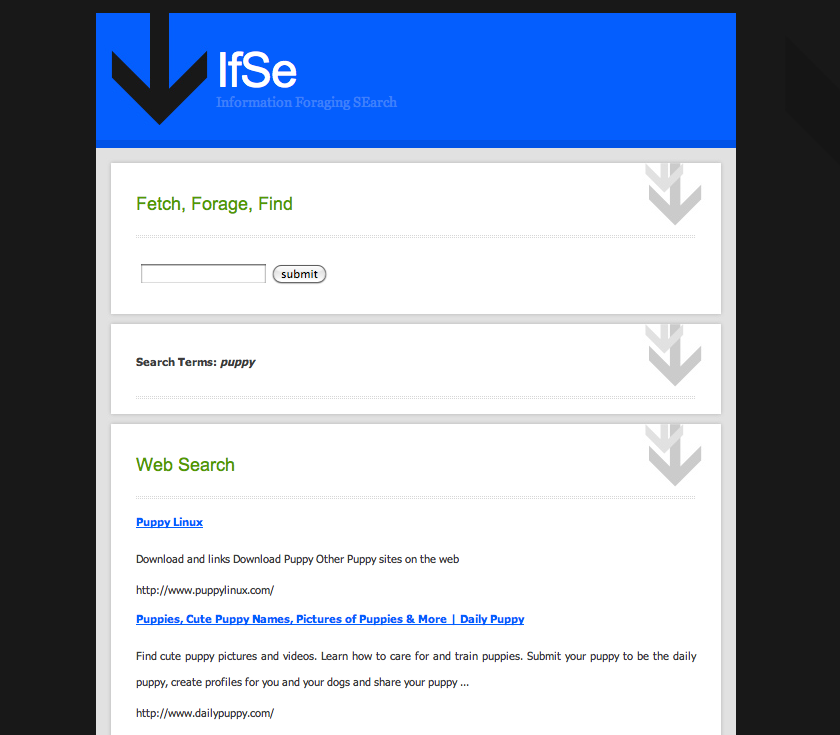
\includegraphics{puppy-ifse-before.png}
\caption{\emph{IfSe running on a local machine.}}\end{figure}

Excellent! You now have a simple search interface that is hooked up to the Bing search API.

Go on, try it out. Search for something!

While, this service means you can search the web, it doesn't record anything.


\subsection{Logging Queries}
\label{ifse-tutorial:logging-queries}
Let's assume that we'd like to keep track of all the queries that users submit so that we can do a query log analysis later on.

There are a number of ways to do this. But let's do it the simple way first.

Load up a code editor and open up \code{ifse/service.py}

This is where we can specify how we would like to configure our search service. We can easily add and modify search engines, query filters and result filters. See {\hyperref[api2.0:api]{\emph{PuppyIR API Reference}}} for more information.

The PuppyIR framework provides a default query logger, lets include it by adding the following lines of code:

\begin{Verbatim}[commandchars=\\\{\}]
\PYG{k+kn}{from} \PYG{n+nn}{puppy.logging} \PYG{k+kn}{import} \PYG{n}{QueryLogger}
\end{Verbatim}

This is a file based query logging. To tell PuppyIR where to store the log we need to add a ``log\_dir'' to the config:

\begin{Verbatim}[commandchars=\\\{\}]
\PYG{n}{config} \PYG{o}{=} \PYG{p}{\PYGZob{}}
    \PYG{l+s}{"}\PYG{l+s}{log\PYGZus{}dir}\PYG{l+s}{"}\PYG{p}{:} \PYG{l+s}{"}\PYG{l+s}{ifse/query\PYGZus{}logs}\PYG{l+s}{"}\PYG{p}{,}
\PYG{p}{\PYGZcb{}}
\end{Verbatim}

After the declaration and creation of the \code{web\_search\_service}, add the following line of code:

\begin{Verbatim}[commandchars=\\\{\}]
\PYG{n}{web\PYGZus{}search\PYGZus{}service}\PYG{o}{.}\PYG{n}{query\PYGZus{}logger} \PYG{o}{=} \PYG{n}{QueryLogger}\PYG{p}{(}\PYG{n}{web\PYGZus{}search\PYGZus{}service}\PYG{p}{,} \PYG{n}{log\PYGZus{}mode}\PYG{o}{=}\PYG{l+m+mi}{0}\PYG{p}{)}
\end{Verbatim}

This tells PuppyIR that you would like log queries that are submitted to this search service.

Too Easy!

Now, make sure the server is still running, i.e. python manage.py runserver and visit \href{http://127.0.0.1:8000/ifse}{http://127.0.0.1:8000/ifse}

Type in a few queries.

Now, go and check the directory \code{ifse/query\_logs}, you should have a file in there called, \code{web\_search\_query\_log}. This will contain a list of the queries that you have just entered. I hope you didn't type in any naughty queries!


\subsection{Modifying Queries}
\label{ifse-tutorial:modifying-queries}
Part of the PuppyIR project is to create child friendly services. So lets add a QueryFilter that stops naughty query terms being submitted to the search engine. To do this, we can use the \code{BlackListFiter} component that is part of the PuppyIR framework. Now add the following line of code to import it:

\begin{Verbatim}[commandchars=\\\{\}]
\PYG{k+kn}{from} \PYG{n+nn}{puppy.query.filter} \PYG{k+kn}{import} \PYG{n}{BlackListFilter}
\end{Verbatim}

Then after the declaration and creation of the web\_search\_service, add the following lines of code:

\begin{Verbatim}[commandchars=\\\{\}]
\PYG{n}{query\PYGZus{}black\PYGZus{}list} \PYG{o}{=} \PYG{n}{BlackListFilter}\PYG{p}{(}\PYG{l+m+mi}{0}\PYG{p}{,} \PYG{n}{terms} \PYG{o}{=} \PYG{l+s}{"}\PYG{l+s}{bad worse nasty filthy}\PYG{l+s}{"}\PYG{p}{)}
\PYG{n}{web\PYGZus{}search\PYGZus{}service}\PYG{o}{.}\PYG{n}{add\PYGZus{}query\PYGZus{}filter}\PYG{p}{(}\PYG{n}{query\PYGZus{}black\PYGZus{}list}\PYG{p}{)}
\end{Verbatim}

What the Blacklist filter does, is, look at the query sent to the PuppyIR framework and check each word contained in it (the query) against the blacklist. The blacklist defines words that are not allowed (in the code example above the blacklist is populated via the second parameter; separated by spaces). If your query contains any of these words then the query will be rejected and a message displayed stating this.

Try the service now. Enter a really naughty query, like ``bad test'' and see what happens. A message should be displayed stating that the query was rejected because it contained blacklisted words.


\subsection{Adding Another Search Service}
\label{ifse-tutorial:adding-another-search-service}
Instead of just returning web results, we might want to all add in other kinds of results. PuppyIR also contains various other search engine wrappers to APIs other than Bing, such as: Twitter, Yahoo, etc. For more details about search engine wrappers see {\hyperref[api2.0:api]{\emph{PuppyIR API Reference}}}

Let's create a new search service, so that we can include Twitter results as well as web results. To do this add the following line of code:

\begin{Verbatim}[commandchars=\\\{\}]
\PYG{k+kn}{from} \PYG{n+nn}{puppy.search.engine} \PYG{k+kn}{import} \PYG{n}{Twitter}
\end{Verbatim}

And then declare and create this new SearchService and search engine, with:

\begin{Verbatim}[commandchars=\\\{\}]
\PYG{n}{twitter\PYGZus{}search\PYGZus{}service} \PYG{o}{=} \PYG{n}{SearchService}\PYG{p}{(}\PYG{n}{service}\PYG{p}{,}\PYG{l+s}{"}\PYG{l+s}{twitter\PYGZus{}search}\PYG{l+s}{"}\PYG{p}{)}
\PYG{n}{twitter\PYGZus{}search\PYGZus{}service}\PYG{o}{.}\PYG{n}{search\PYGZus{}engine} \PYG{o}{=} \PYG{n}{Twitter}\PYG{p}{(}\PYG{n}{twitter\PYGZus{}search\PYGZus{}service}\PYG{p}{)}
\end{Verbatim}

Don't forget to add it to the PuppyIR service manager, which is called service:

\begin{Verbatim}[commandchars=\\\{\}]
\PYG{n}{service}\PYG{o}{.}\PYG{n}{add\PYGZus{}search\PYGZus{}service}\PYG{p}{(}\PYG{n}{twitter\PYGZus{}search\PYGZus{}service}\PYG{p}{)}
\end{Verbatim}

Okay, let's try the service out now. When you enter a query now, it should return two panes of results: first, the web results and then the twitter results.

Wow! How cool is that?


\subsection{More Querying Logging}
\label{ifse-tutorial:more-querying-logging}
The query logger above simply dumps all the queries entered to a flat file. While this is really handy to process afterwards, it would be nice if we could index all the queries and then present similar queries as query suggestions.

To do this we need two include two components, a \code{QueryFilter} that records and indexes queries submitted to the service, and a \code{SearchService} that recommends queries. Luckily we have already implemented a simple query indexing \code{QueryFilter} that uses the Python based Whoosh indexer. The filter is called, \code{WhooshQueryLogger}, while the search engine is called \code{WhooshQueryEngine}. Let's import then into our \code{service.py}:

\begin{Verbatim}[commandchars=\\\{\}]
\PYG{k+kn}{from} \PYG{n+nn}{puppy.query.filter.whooshQueryLogger} \PYG{k+kn}{import} \PYG{n}{WhooshQueryLogger}
\PYG{k+kn}{from} \PYG{n+nn}{puppy.search.engine.whooshQueryEngine} \PYG{k+kn}{import} \PYG{n}{WhooshQueryEngine}
\end{Verbatim}

Now create the \code{WhooshQueryLogger}. It will need the full path name to the index directory. And then it needs to be added to the \code{search\_service} that we wish to log, so here we can log the \code{web\_search\_service}:

\begin{Verbatim}[commandchars=\\\{\}]
\PYG{n}{whoosh\PYGZus{}dir} \PYG{o}{=} \PYG{n}{os}\PYG{o}{.}\PYG{n}{path}\PYG{o}{.}\PYG{n}{join}\PYG{p}{(}\PYG{n}{os}\PYG{o}{.}\PYG{n}{getcwd}\PYG{p}{(}\PYG{p}{)}\PYG{p}{,} \PYG{l+s}{"}\PYG{l+s}{ifse/query\PYGZus{}logs/index}\PYG{l+s}{"}\PYG{p}{)}
\PYG{n}{whoosh\PYGZus{}query\PYGZus{}logger} \PYG{o}{=} \PYG{n}{WhooshQueryLogger}\PYG{p}{(}\PYG{n}{whoosh\PYGZus{}query\PYGZus{}index\PYGZus{}dir}\PYG{o}{=}\PYG{n}{whoosh\PYGZus{}dir}\PYG{p}{,} \PYG{n}{unique}\PYG{o}{=}\PYG{n+nb+bp}{True}\PYG{p}{)}
\PYG{n}{web\PYGZus{}search\PYGZus{}service}\PYG{o}{.}\PYG{n}{add\PYGZus{}query\PYGZus{}filter}\PYG{p}{(}\PYG{n}{whoosh\PYGZus{}query\PYGZus{}logger}\PYG{p}{)}
\end{Verbatim}

Now, we want to provide the suggestions, so we need to create a SearchService for query suggestions and then create the WhooshQueryEngine, which also needs to know the location of the index directory:

\begin{Verbatim}[commandchars=\\\{\}]
\PYG{n}{suggest\PYGZus{}service} \PYG{o}{=} \PYG{n}{SearchService}\PYG{p}{(}\PYG{n}{service}\PYG{p}{,} \PYG{l+s}{"}\PYG{l+s}{query\PYGZus{}suggest\PYGZus{}search}\PYG{l+s}{"}\PYG{p}{)}
\PYG{n}{whoosh\PYGZus{}engine} \PYG{o}{=} \PYG{n}{WhooshQueryEngine}\PYG{p}{(}\PYG{n}{suggest\PYGZus{}service}\PYG{p}{,} \PYG{n}{whoosh\PYGZus{}query\PYGZus{}index\PYGZus{}dir}\PYG{o}{=}\PYG{n}{whoosh\PYGZus{}dir}\PYG{p}{)}
\PYG{n}{suggest\PYGZus{}service}\PYG{o}{.}\PYG{n}{search\PYGZus{}engine} \PYG{o}{=} \PYG{n}{whoosh\PYGZus{}engine}
\PYG{n}{service}\PYG{o}{.}\PYG{n}{add\PYGZus{}search\PYGZus{}service}\PYG{p}{(}\PYG{n}{suggest\PYGZus{}service}\PYG{p}{)}
\end{Verbatim}

Okay, so let's start entering a few queries. Note, you might have to enter a few queries before you start to see recommendations appearing.


\subsection{Pipelining}
\label{ifse-tutorial:pipelining}
You might notice that if you type in ``bad query'', you still get results for the twitter service. This is because we didn't add the \code{BlackListFilter} to our \code{twitter\_search\_service}. Do that now and make sure nothing nasty gets through.

Also, if we added the \code{WhooshQueryLogger} before the \code{BlackListFilter} then we would record all the nasty queries before rejecting the query and then start to recommend them....ooops! So it is always a good idea to pay attention to your query and document pipelines.


\subsection{Give IfSe a Style}
\label{ifse-tutorial:give-ifse-a-style}
If you are interested in changing the look and feel of the application, then you can check out the html template files in \code{templates/ifse/} within the tutorial directory, and the corresponding style sheet held in, \code{site\_media/css/}

For example, open up \code{index.html} in \code{template/ifse} and change:

\begin{Verbatim}[commandchars=\\\{\}]
\textless{}link href="\PYGZob{}\PYGZob{} MEDIA\_URL \PYGZcb{}\PYGZcb{}css/concurrence/style.css" rel="stylesheet"  type="text/css"\textgreater{}
\end{Verbatim}

to:

\begin{Verbatim}[commandchars=\\\{\}]
\textless{}link href="\PYGZob{}\PYGZob{} MEDIA\_URL \PYGZcb{}\PYGZcb{}css/twirling/style.css" rel="stylesheet"  type="text/css"\textgreater{}
\end{Verbatim}

Doesn't IfSe look prettier in pink?

Try changing \code{perplex} to \code{combination}, \code{passageway}, \code{twirling} or download any other CSS style from
\href{http://freecsstemplates.org}{http://freecsstemplates.org}.


\subsection{Summing Up}
\label{ifse-tutorial:summing-up}
In this tutorial, we have only considered how to configure a service using some of the existing components within the PuppyIR framework. But it is really easy to develop your own components and customise your search service. To develop your own components, check out {\hyperref[extendingQuery:extending-the-query-pipeline]{\emph{Extending the Query Pipeline}}}, {\hyperref[extendingResult:extending-the-result-pipeline]{\emph{Extending the Result Pipeline}}} and {\hyperref[extendingSearchEngine:extending-the-search-engine]{\emph{Adding new Search Engine Wrappers}}} for more details.


\section{MaSe Tutorial: Mash-up Search Engine Application}
\label{mase-tutorial:mase-mash-up-search-engine-puppyir-tutorial}\label{mase-tutorial:mase-tutorial-mash-up-search-engine-application}\label{mase-tutorial::doc}

\subsection{Getting Started}
\label{mase-tutorial:getting-started}
Before starting this tutorial we assume that you have downloaded and installed the PuppyIR framework along with required associated Python Libraries (this tutorial also requires Whoosh to be installed).

If you have not installed the PuppyIR framework and/or Whoosh go to {\hyperref[installation:requirements-and-installation]{\emph{Requirements and Installation}}} and get everything set up.

This tutorial is designed to show the PuppyIR framework can be used to create and customise a web application, quickly, using the Django web framework. No Python experience is required to do this tutorial, as there is minimal coding involved and there are instructions regarding what coding there is (failing that, an answer file is included called `\emph{complete-service.py}` which includes working code for all the tasks).

Please note that Javascript must be enabled for this tutorial to work, ask your teacher if this is the case and, if not, get them to enable Javascript.


\subsubsection{Downloading the Source Code for the Tutorial}
\label{mase-tutorial:downloading-the-source-code-for-the-tutorial}
Now that you've got PuppyIR, Django and Whoosh installed it's time to download the latest release of the tutorial from the PuppyIR repository using the following command (if you have problems with this step please ask your teacher for help):

\begin{Verbatim}[commandchars=\\\{\}]
\$ svn co https://puppyir.svn.sourceforge.net/svnroot/puppyir/trunk/prototypes/mase-tutorial
\end{Verbatim}

N.B. depending on your OS and SVN version you may need to add ` mase-tutorial' to the end of the above command.


\subsubsection{Run MaSe}
\label{mase-tutorial:run-mase}
To run MaSe, execute the following two commands (substituting in the path to where you downloaded MaSe to):

\begin{Verbatim}[commandchars=\\\{\}]
\$ cd /path/to/mase-tutorial
\$ python manage.py runserver
\end{Verbatim}

Now, visit: \href{http://localhost:8000/mase}{http://localhost:8000/mase} which should bring up the screen shown below (if you are using Internet Explorer you will not get rounded edges for your result boxes):
\begin{figure}[htbp]
\centering
\capstart

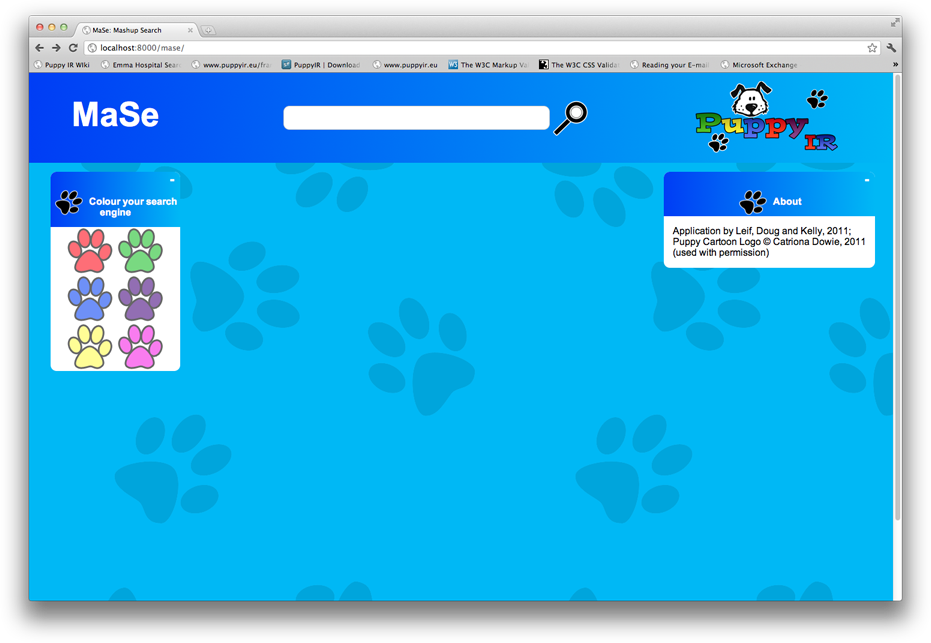
\includegraphics{mase-1-initial.png}
\caption{\emph{MaSe running on a local machine.}}\end{figure}

To search for results either press enter/return in the search box or click on the magnifying glass.

You can customise your search engine by:
\begin{enumerate}
\item {} 
Clicking on the title, `MaSe', allows you to change the name of the search engine by typing in a new name - pressing enter/return will save your search engine's new name.

\item {} 
Clicking on the paw images in the `\textbf{Colour your search engine}` box will change the colour theme of the search engine.

\item {} 
You can also move the result boxes around on the screen (more on this in the next section).

\item {} 
Minimise results by clicking on the `\textbf{-}` on the top right of a result box; you can maximise it again by clicking on the `\textbf{+}` that appears when results are minimised.

\end{enumerate}

Go ahead and name your search engine and pick a new colour scheme - your new settings will be saved (using cookies; ask your teacher to enable cookies if they are disabled) so there is no need to do this every time.


\subsection{Adding our first services}
\label{mase-tutorial:adding-our-first-services}
However, we don't have any services added yet, so, will get no results when searching. Let's fix that now by adding our first service: web results. Open the `\emph{service.py}` file in the \emph{mase} directory and add the following lines of code, at the bottom of the file(the code comments, the lines starting with `\#', detail the purpose of each line) :

\begin{Verbatim}[commandchars=\\\{\}]
\PYG{c}{\PYGZsh{} create a SearchService, called 'web\PYGZus{}search'}
\PYG{n}{web\PYGZus{}search\PYGZus{}service} \PYG{o}{=} \PYG{n}{SearchService}\PYG{p}{(}\PYG{n}{service}\PYG{p}{,} \PYG{l+s}{"}\PYG{l+s}{web\PYGZus{}search}\PYG{l+s}{"}\PYG{p}{)}

\PYG{c}{\PYGZsh{} Set our SearchService to use the Bing search engine (it defaults to search for web results)}
\PYG{n}{web\PYGZus{}search\PYGZus{}service}\PYG{o}{.}\PYG{n}{search\PYGZus{}engine} \PYG{o}{=} \PYG{n}{Bing}\PYG{p}{(}\PYG{n}{web\PYGZus{}search\PYGZus{}service}\PYG{p}{)}

\PYG{c}{\PYGZsh{} add SearchService to our ServiceManager (this handles all the search services MaSe contains)}
\PYG{n}{service}\PYG{o}{.}\PYG{n}{add\PYGZus{}search\PYGZus{}service}\PYG{p}{(}\PYG{n}{web\PYGZus{}search\PYGZus{}service}\PYG{p}{)}
\end{Verbatim}

Now refresh your browser and search for something. You should be presented with results, for your query, in a format similar to what is shown below:
\begin{figure}[htbp]
\centering
\capstart

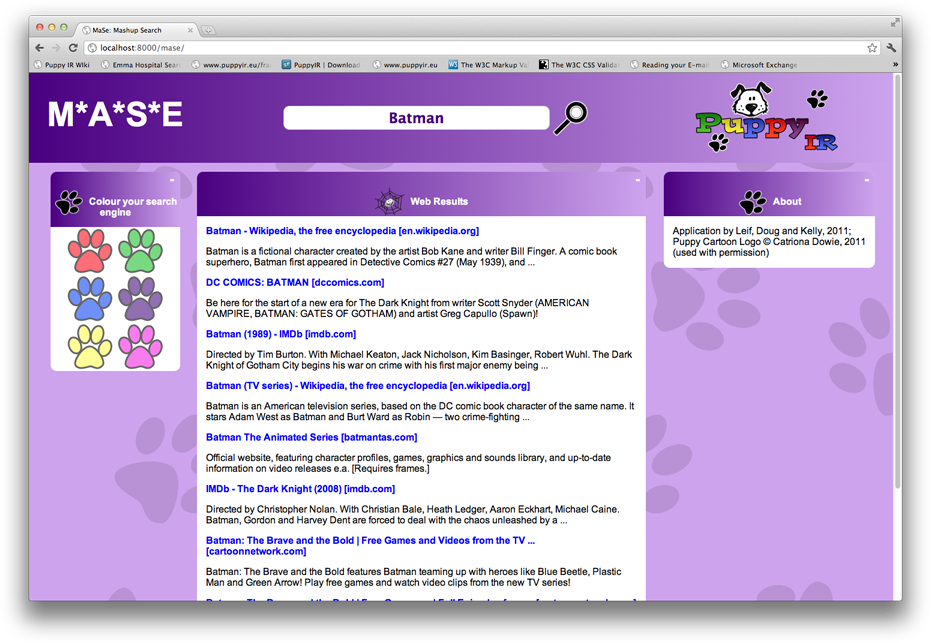
\includegraphics{mase-3-web.png}
\caption{\emph{Our now customised MaSe (custom title and new colour scheme) showing web results.}}\end{figure}

Now, lets limit the number of web results to only three, this is done by changing the line of code with `\textbf{Bing}` in it to:

\begin{Verbatim}[commandchars=\\\{\}]
\PYG{c}{\PYGZsh{} Set the resultsPerPage parameter to 3; this limits the results the service will return}
\PYG{n}{web\PYGZus{}search\PYGZus{}service}\PYG{o}{.}\PYG{n}{search\PYGZus{}engine} \PYG{o}{=} \PYG{n}{Bing}\PYG{p}{(}\PYG{n}{web\PYGZus{}search\PYGZus{}service}\PYG{p}{,} \PYG{n}{resultsPerPage} \PYG{o}{=} \PYG{l+m+mi}{3}\PYG{p}{)}
\end{Verbatim}

But, it's boring just having one set of results - so lets add images as well. This is done by adding the code below (note the differences and similarities to adding web results):

\begin{Verbatim}[commandchars=\\\{\}]
\PYG{c}{\PYGZsh{} create a SearchService, called 'image\PYGZus{}search'}
\PYG{n}{image\PYGZus{}service} \PYG{o}{=} \PYG{n}{SearchService}\PYG{p}{(}\PYG{n}{service}\PYG{p}{,} \PYG{l+s}{"}\PYG{l+s}{image\PYGZus{}search}\PYG{l+s}{"}\PYG{p}{)}

\PYG{c}{\PYGZsh{} Set our SearchService to use Bing but this time with images}
\PYG{n}{image\PYGZus{}service}\PYG{o}{.}\PYG{n}{search\PYGZus{}engine} \PYG{o}{=} \PYG{n}{Bing}\PYG{p}{(}\PYG{n}{image\PYGZus{}service}\PYG{p}{,} \PYG{n}{source}\PYG{o}{=}\PYG{l+s}{'}\PYG{l+s}{image}\PYG{l+s}{'}\PYG{p}{,} \PYG{n}{resultsPerPage} \PYG{o}{=} \PYG{l+m+mi}{3}\PYG{p}{)}

\PYG{c}{\PYGZsh{} add SearchService to our ServiceManager}
\PYG{n}{service}\PYG{o}{.}\PYG{n}{add\PYGZus{}search\PYGZus{}service}\PYG{p}{(}\PYG{n}{image\PYGZus{}service}\PYG{p}{)}
\end{Verbatim}

Go ahead and search for something, you should now see images and web results. You can also drag your results around and place them either on the left, centre, or right result columns; an example of this is shown below:
\begin{figure}[htbp]
\centering
\capstart

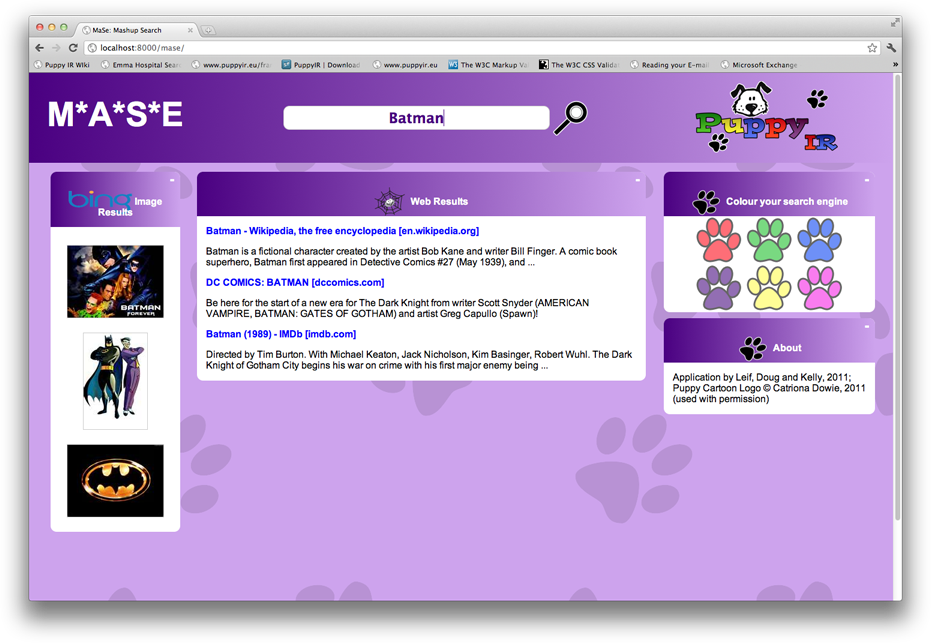
\includegraphics{mase-4-webimages.png}
\caption{\emph{Re-arranging `Web' and `Image' results in MaSe.}}\end{figure}


\subsection{Extending MaSe with query logging and suggestions}
\label{mase-tutorial:extending-mase-with-query-logging-and-suggestions}
Now let's add a query logger to record our queries by adding the code below just after where we created (and added) the web search service:

\begin{Verbatim}[commandchars=\\\{\}]
\PYG{c}{\PYGZsh{} Create a Whoosh Query Logger that records all the unique queries}
\PYG{n}{whoosh\PYGZus{}query\PYGZus{}logger} \PYG{o}{=} \PYG{n}{WhooshQueryLogger}\PYG{p}{(}\PYG{n}{whoosh\PYGZus{}query\PYGZus{}index\PYGZus{}dir}\PYG{o}{=}\PYG{n}{whoosh\PYGZus{}dir}\PYG{p}{,} \PYG{n}{unique}\PYG{o}{=}\PYG{n+nb+bp}{True}\PYG{p}{)}

\PYG{c}{\PYGZsh{} Add the Whoosh Query Logger to the web\PYGZus{}search service}
\PYG{n}{web\PYGZus{}search\PYGZus{}service}\PYG{o}{.}\PYG{n}{add\PYGZus{}query\PYGZus{}filter}\PYG{p}{(}\PYG{n}{whoosh\PYGZus{}query\PYGZus{}logger}\PYG{p}{)}
\end{Verbatim}

Next we want query suggestions, add the following lines of code to enable this feature:

\begin{Verbatim}[commandchars=\\\{\}]
\PYG{c}{\PYGZsh{} create a SearchService, called 'query\PYGZus{}suggest\PYGZus{}search'}
\PYG{n}{suggest\PYGZus{}service} \PYG{o}{=} \PYG{n}{SearchService}\PYG{p}{(}\PYG{n}{service}\PYG{p}{,} \PYG{l+s}{"}\PYG{l+s}{query\PYGZus{}suggest\PYGZus{}search}\PYG{l+s}{"}\PYG{p}{)}

\PYG{c}{\PYGZsh{} Use the Whoosh Query Engine to record queries}
\PYG{n}{whooshEngine} \PYG{o}{=} \PYG{n}{WhooshQueryEngine}\PYG{p}{(}\PYG{n}{suggest\PYGZus{}service}\PYG{p}{,} \PYG{n}{whoosh\PYGZus{}query\PYGZus{}index\PYGZus{}dir}\PYG{o}{=}\PYG{n}{whoosh\PYGZus{}dir}\PYG{p}{)}
\PYG{n}{suggest\PYGZus{}service}\PYG{o}{.}\PYG{n}{search\PYGZus{}engine} \PYG{o}{=} \PYG{n}{whooshEngine}

\PYG{c}{\PYGZsh{} add SearchService to our ServiceManager}
\PYG{n}{service}\PYG{o}{.}\PYG{n}{add\PYGZus{}search\PYGZus{}service}\PYG{p}{(}\PYG{n}{suggest\PYGZus{}service}\PYG{p}{)}
\end{Verbatim}

What the `\emph{suggest\_service} does is to look at past queries and see if any of them contain terms from the current query. If so, it recommends those past queries as suggestions. The picture below shows query suggestions in action. Go ahead and enter a few queries now; to test if the query suggestions are working.
\begin{figure}[htbp]
\centering
\capstart

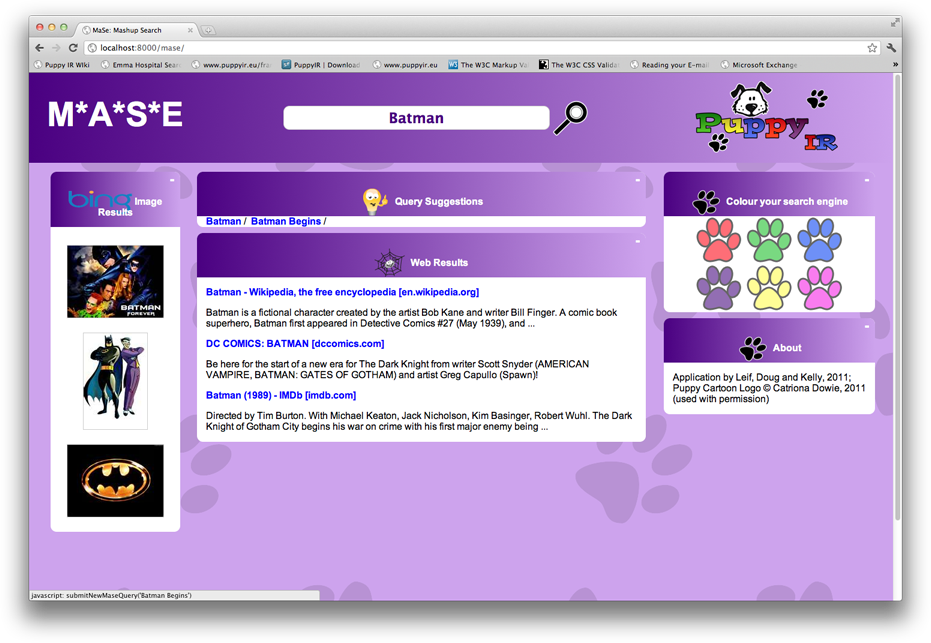
\includegraphics{mase-5-limitresults.png}
\caption{\emph{MaSe showing our now limited results for each service and query suggestions.}}\end{figure}


\subsection{Filtering and the Pipelining}
\label{mase-tutorial:filtering-and-the-pipelining}
Now that we've got results from three sources, lets add some filtering to stop people using your search engine to search for certain keywords. After the creation of the web\_search\_service, add the following lines of code to add a `\textbf{BlackListFilter}`:

\begin{Verbatim}[commandchars=\\\{\}]
\PYG{c}{\PYGZsh{} Create a blacklist filter to block queries containing the terms below}
\PYG{n}{query\PYGZus{}black\PYGZus{}list} \PYG{o}{=} \PYG{n}{BlackListFilter}\PYG{p}{(}\PYG{n}{terms} \PYG{o}{=} \PYG{l+s}{"}\PYG{l+s}{bad worse nasty filthy}\PYG{l+s}{"}\PYG{p}{)}

\PYG{c}{\PYGZsh{} Add our blacklist filter to the web search service}
\PYG{n}{web\PYGZus{}search\PYGZus{}service}\PYG{o}{.}\PYG{n}{add\PYGZus{}query\PYGZus{}filter}\PYG{p}{(}\PYG{n}{query\PYGZus{}black\PYGZus{}list}\PYG{p}{)}
\end{Verbatim}

You will notice that if you type in ``bad query'', you still get results for the image service. This is because we didn't add the `\textbf{BlackListFilter}` to our `\emph{image\_service}`. Do that now and make sure nothing nasty gets through.

Also, if we added the `\textbf{WhooshQueryLogger}` before the `\textbf{BlackListFilter}` then we would record all the nasty queries before rejecting the query and then start to recommend them as suggestions.... ooops! So it is always a good idea to pay attention to your query and document pipelines - re-order these now to stop any bad suggestions being recommended.
\begin{figure}[htbp]
\centering
\capstart

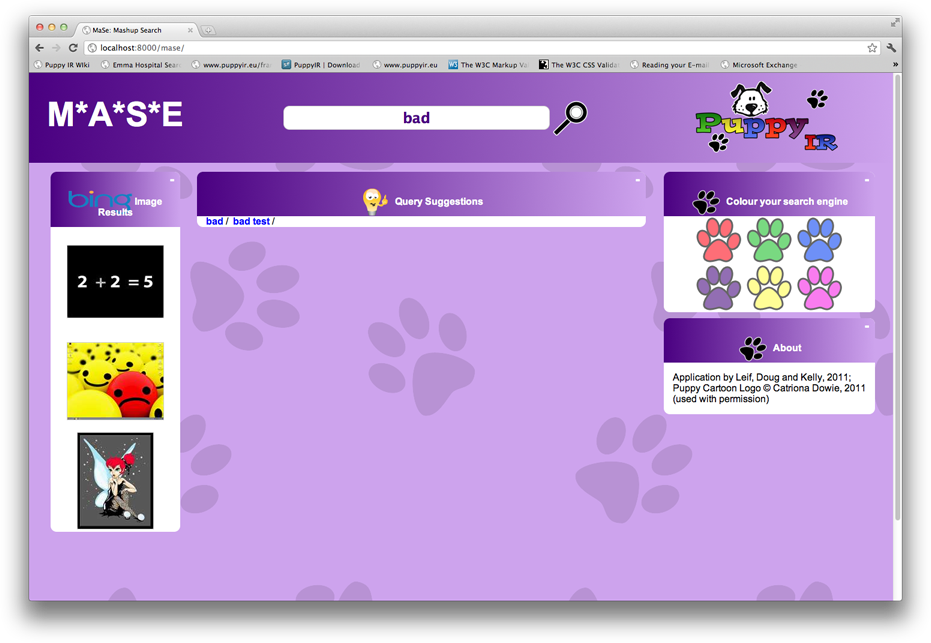
\includegraphics{mase-6-badsuggestions.png}
\caption{\emph{MaSe making bad suggestions and still showing image results; as in this case the filter was not added to image search}}\end{figure}


\subsection{Experimenting}
\label{mase-tutorial:experimenting}
Well done, that's you completed the tutorial :) - what's next is up to you, if you want to do more the following two sections contain details for suggestions for extending your search engine further.


\subsubsection{Other Services}
\label{mase-tutorial:other-services}
So far you've added images, web and query suggestions to MaSe but there's more available.

The table below details the other options (see the code for `\emph{web\_search\_service}` and adapt it using the details below):

\begin{tabulary}{\linewidth}{|L|L|L|L|}
\hline
\textbf{
Result Source
} & \textbf{
Service Name
} & \textbf{
Class Name
} & \textbf{
Extra parameters
}\\\hline

Wikipedia
 & 
\emph{wiki\_search}
 & 
\textbf{Wikipedia}
 & \\\hline

Bing News
 & 
\emph{news\_search}
 & 
\textbf{Bing}
 & 
source='news'
\\\hline

Video (Youtube)
 & 
\emph{video\_search}
 & 
\textbf{YouTubeV2}
 & \\\hline

Twitter
 & 
\emph{twitter\_search}
 & 
\textbf{Twitter}
 & \\\hline
\end{tabulary}


If you get stuck adding the above services then look at the file `\emph{service-complete.py}` which includes working code to add them.

You can also add in past queries with the following code (change `web\_search\_service' to whatever service to want to log queries for):

\begin{Verbatim}[commandchars=\\\{\}]
\PYG{c}{\PYGZsh{} Log queries sent to the web search service}
\PYG{n}{web\PYGZus{}search\PYGZus{}service}\PYG{o}{.}\PYG{n}{query\PYGZus{}logger} \PYG{o}{=} \PYG{n}{QueryLogger}\PYG{p}{(}\PYG{n}{web\PYGZus{}search\PYGZus{}service}\PYG{p}{,} \PYG{n}{log\PYGZus{}mode}\PYG{o}{=}\PYG{l+m+mi}{0}\PYG{p}{)}
\end{Verbatim}
\begin{figure}[htbp]
\centering
\capstart

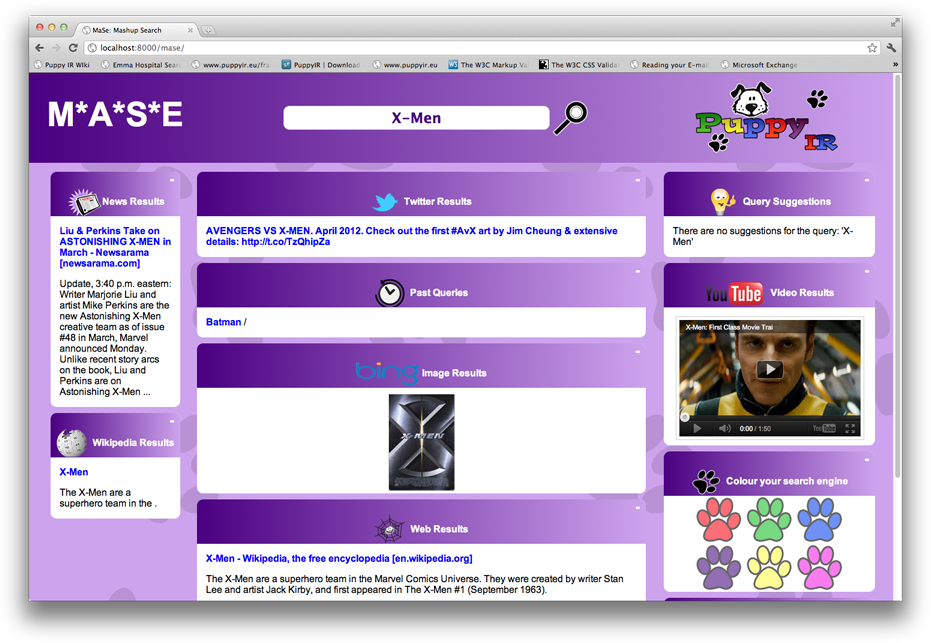
\includegraphics{mase-7-all.png}
\caption{\emph{MaSe with all the different result types added to it.}}\end{figure}

The picture above shows what MaSe looks like with all the above services added to it with the results limited to only show the top result.


\subsubsection{Other Parameters}
\label{mase-tutorial:other-parameters}
There are also a few other parameters you can try out for the video and twitter services beyond `resultsPerPage':
\begin{itemize}
\item {} 
\textbf{Video} orderBy (string), can be: `rating', `viewCount' or `relevance'

\item {} 
\textbf{Twitter} language (string), `en' for English, `de' for German; type (string), can be: `mixed', `recent' or `popular'

\end{itemize}


\section{Pipeline Tutorial: DeeSe (Detective Search)}
\label{pipeline-tutorial:pipeline-puppyir-tutorial}\label{pipeline-tutorial:pipeline-tutorial-deese-detective-search}\label{pipeline-tutorial::doc}

\subsection{Getting Started}
\label{pipeline-tutorial:getting-started}
If you have not installed the PuppyIR framework and/or Django, please go to {\hyperref[installation:requirements-and-installation]{\emph{Requirements and Installation}}} to get everything set up. Also, before starting this tutorial, it is recommended that you read the background page on the pipeline paradigm, {\hyperref[pipeline:pipeline-architecture]{\emph{Paradigm 2 - One Pipeline, Many Search Engines}}}, as this provides a conceptual description of how the paradigm works.

The first step is to checkout the tutorial from the PuppyIR SourceForge page and run it with the following commands:

\begin{Verbatim}[commandchars=\\\{\}]
\$ svn co https://puppyir.svn.sourceforge.net/svnroot/puppyir/trunk/prototypes/deese-tutorial
\$ cd /path/to/deese-tutorial
\$ python manage.py runserver
\end{Verbatim}

N.B. depending on your OS and SVN version, you may need to add ` deese-tutorial' to the end of the above svn checkout command.

Now visit: \href{http://localhost:8000/deese}{http://localhost:8000/deese} to see the initial version of the application.

If you get stuck, at any point, during this tutorial, please consult the `service-complete.py' file in the \emph{`deese'} folder, this contains the ``answer'' to this tutorial; along with code comments explaining each step.


\subsection{DeeSee background}
\label{pipeline-tutorial:deesee-background}
This tutorial is, in a sense, a companion piece to the BaSe and IfSe tutorials in that it shows how to implement similar functionality using the `pipeline' paradigm. The scenario in this tutorial  concerns a situation where the `pipeline' paradigm is more suited the application than the `service' paradigm.

The scenario is: you are working on an application for a team of Detectives to enable them to investigate several suspects (who have been stealing data off online websites). These suspects are well versed in electronic communication and are keeping a watch on the search history of the Detective Agency (by looking at queries sent and for their names appearing in the results the Detectives are viewing). To this end, DeeSe aims to provide the ability to search multiple sources, but have queries and results modified to prevent the names of the suspects appearing.

Therefore, for all the search services being used, one specific pipeline (for queries and results) needs to be put in place to enforce the `lack of the suspects name' rule. Now, with the `service' paradigm we would need to construct this pipeline for each and every source, but could we do it a different way? This tutorial details how, using the `pipeline' paradigm, this could be accomplished.


\subsection{Creating our Pipeline Service}
\label{pipeline-tutorial:creating-our-pipeline-service}
The first step is to create a pipeline service for DeeSe (the pipeline service has already been done for you; but note how to do it) and add a search engine to it. Open up `service.py' in the DeeSe directory and enter the following code (after the comment saying start here):

\begin{Verbatim}[commandchars=\\\{\}]
\PYG{c}{\PYGZsh{} Create our Pipeline Service}
\PYG{n}{pipelineService} \PYG{o}{=} \PYG{n}{PipelineService}\PYG{p}{(}\PYG{n}{config}\PYG{p}{,} \PYG{l+s}{"}\PYG{l+s}{myPipeline}\PYG{l+s}{"}\PYG{p}{)}

\PYG{c}{\PYGZsh{} ----------------------- Start Here -----------------------}

\PYG{c}{\PYGZsh{} Create a Bing Search Engine for news results and limit to 5 results}
\PYG{n}{bingNews} \PYG{o}{=} \PYG{n}{Bing}\PYG{p}{(}\PYG{n}{pipelineService}\PYG{p}{,} \PYG{n}{source}\PYG{o}{=}\PYG{l+s}{'}\PYG{l+s}{news}\PYG{l+s}{'}\PYG{p}{,} \PYG{n}{resultsPerPage}\PYG{o}{=}\PYG{l+m+mi}{5}\PYG{p}{)}

\PYG{c}{\PYGZsh{} Add Bing News to our search engine manager (this stores all our search engines)}
\PYG{n}{pipelineService}\PYG{o}{.}\PYG{n}{searchEngineManager}\PYG{o}{.}\PYG{n}{add\PYGZus{}search\PYGZus{}engine}\PYG{p}{(}\PYG{l+s}{"}\PYG{l+s}{News}\PYG{l+s}{"}\PYG{p}{,} \PYG{n}{bingNews}\PYG{p}{)}
\end{Verbatim}

What this code does is to create a pipeline service and add one search engine to it (Bing News). We can now search for Bing News results using the application's searchbox. However, there is no filtering yet implemented... we should start creating our pipeline.


\subsection{Setting up our query pipeline}
\label{pipeline-tutorial:setting-up-our-query-pipeline}
Currently our query pipeline is empty (it contains no filters or modifiers) and so, will allow us to search using the suspects name; thus alerting them to the investigation. Lets stop this by constructing a query pipeline that will stop this from happening. To this end, we're going to add a query filter called `black list filter', which will reject queries if they contain blacklisted word(s). Let's assume that the suspects are called: Bob and Nathan. Let's get coding:

\begin{Verbatim}[commandchars=\\\{\}]
\PYG{c}{\PYGZsh{} Let's define a variable storing the names of the suspects}
\PYG{n}{suspects} \PYG{o}{=} \PYG{l+s}{'}\PYG{l+s}{Bob Nathan}\PYG{l+s}{'} \PYG{c}{\PYGZsh{} Separated by spaces}

\PYG{c}{\PYGZsh{} Now let's create a black list query filter using the suspects variable}
\PYG{n}{blacklistF} \PYG{o}{=} \PYG{n}{BlackListFilter}\PYG{p}{(}\PYG{n}{terms}\PYG{o}{=}\PYG{n}{suspects}\PYG{p}{)}

\PYG{c}{\PYGZsh{} Add it to our pipeline service's query pipeline}
\PYG{n}{pipelineService}\PYG{o}{.}\PYG{n}{add\PYGZus{}query\PYGZus{}filter}\PYG{p}{(}\PYG{n}{blacklistF}\PYG{p}{)}
\end{Verbatim}

Now, if you're confident this will work, let's try searching for `Nathan the train job' - since one of the thefts involved a rail company. Did it work (you should get a message saying the query was rejected)? If it did, lets move onto the next stage; if not, check your code against the code above or ask for help.


\subsection{But what about the results?}
\label{pipeline-tutorial:but-what-about-the-results}
The other required condition was that the results returned should not contain the suspects names. For this we need to create a result pipeline to process the results. Let's add a black list modifier, what this does is ``censor'' blacklisted words (by replacing them with *'s); thus, we can use this to ensure the suspects names do not appear. While we're at it, lets also add a profanity filter to stop queries containing naughty words.

\begin{Verbatim}[commandchars=\\\{\}]
\PYG{c}{\PYGZsh{} Let's add a Black List Modifier to alter the results}
\PYG{n}{blacklistM} \PYG{o}{=} \PYG{n}{BlackListResultModifier}\PYG{p}{(}\PYG{n}{terms}\PYG{o}{=}\PYG{n}{suspects}\PYG{p}{)}

\PYG{c}{\PYGZsh{} Also, as an extra, let's stop any naughty words}
\PYG{n}{profanityF} \PYG{o}{=} \PYG{n}{WdylProfanityQueryFilter}\PYG{p}{(}\PYG{p}{)}

\PYG{c}{\PYGZsh{} Now let's use the add filters method to add both in one go}
\PYG{n}{pipelineService}\PYG{o}{.}\PYG{n}{add\PYGZus{}filters}\PYG{p}{(}\PYG{n}{profanityF}\PYG{p}{,} \PYG{n}{blacklistM}\PYG{p}{)}
\end{Verbatim}

Try it out, can you think of queries that, while not containing the suspects names, will return results containing their names?

For the purposes of the Detective Agencies internal monitoring, all queries, both un-processed and processed (after going through the query pipeline), should be logged. Let's add a query logger to our pipeline service and set it to log processed queries (as well as the un-processed queries).

\begin{Verbatim}[commandchars=\\\{\}]
\PYG{c}{\PYGZsh{} Create a Query Logger and attach it to our Pipeline Service}
\PYG{n}{pipelineService}\PYG{o}{.}\PYG{n}{query\PYGZus{}logger} \PYG{o}{=} \PYG{n}{QueryLogger}\PYG{p}{(}\PYG{n}{pipelineService}\PYG{p}{)}

\PYG{c}{\PYGZsh{} Set post logging to true i.e. log processed queries (post query pipeline)}
\PYG{n}{pipelineService}\PYG{o}{.}\PYG{n}{postLogging} \PYG{o}{=} \PYG{n+nb+bp}{True}
\end{Verbatim}

Now, search with both valid and invalid queries (i.e. ones that should be rejected). Open the log file (located in the \emph{`deese\_logs'} directory) and take a look at your query history. Note that queries that were not rejected are logged twice (un-processed and processed) and that rejected queries are only logged once. This is because when a query is rejected the search is aborted so there never is a processed query. Also, since we never added any query modifiers the processed queries are the same as their un-processed counterpart.


\subsection{Let's add some new search services}
\label{pipeline-tutorial:let-s-add-some-new-search-services}
Of course, just searching Bing News does not really offer the multiple search services required; let's add Wikipedia and Bing Web as well:

\begin{Verbatim}[commandchars=\\\{\}]
\PYG{c}{\PYGZsh{} Create Bing Web and Wikipedia Search Engines (again, limiting to 5 results)}
\PYG{n}{bingWeb} \PYG{o}{=} \PYG{n}{Bing}\PYG{p}{(}\PYG{n}{pipelineService}\PYG{p}{,} \PYG{n}{source}\PYG{o}{=}\PYG{l+s}{'}\PYG{l+s}{web}\PYG{l+s}{'}\PYG{p}{,} \PYG{n}{resultsPerPage}\PYG{o}{=}\PYG{l+m+mi}{5}\PYG{p}{)}
\PYG{n}{wikipedia} \PYG{o}{=} \PYG{n}{Wikipedia}\PYG{p}{(}\PYG{n}{pipelineService}\PYG{p}{,} \PYG{n}{resultsPerPage}\PYG{o}{=}\PYG{l+m+mi}{5}\PYG{p}{)}

\PYG{c}{\PYGZsh{} Add our new Search Engines to our Search Engine Manager}
\PYG{n}{pipelineService}\PYG{o}{.}\PYG{n}{searchEngineManager}\PYG{o}{.}\PYG{n}{add\PYGZus{}search\PYGZus{}engine}\PYG{p}{(}\PYG{l+s}{"}\PYG{l+s}{Web}\PYG{l+s}{"}\PYG{p}{,} \PYG{n}{bingWeb}\PYG{p}{)}
\PYG{n}{pipelineService}\PYG{o}{.}\PYG{n}{searchEngineManager}\PYG{o}{.}\PYG{n}{add\PYGZus{}search\PYGZus{}engine}\PYG{p}{(}\PYG{l+s}{"}\PYG{l+s}{Wikipedia}\PYG{l+s}{"}\PYG{p}{,} \PYG{n}{wikipedia}\PYG{p}{)}
\end{Verbatim}

Now search for something, notice that the results appear for all of these search engines using the name we supplied: Web, Wikipedia, News as the title. Also, we did not need to alter `views.py' to get results from the new search engines (which you would have to do if using the `service' paradigm). This is because we are using the `searchAll' method call; you could also search them one by one using `searchSpecific' - which makes use of the name of the search engine. Due to this, we can easily add and remove search engines as required.

As an extension task, to allow you to fully understand how DeeSe allows new search engines to be added, have a look at the `index.html' template. The Django template language code is fully commented, explaining the purpose of each line and how the results of each service are accessed \& displayed (also note how the template only shows details about a search engine if it returned one or more results). This is an example of how the overall results dictionary (see: {\hyperref[pipeline:pipeline-architecture]{\emph{Paradigm 2 - One Pipeline, Many Search Engines}}}) can be processed by an application.


\subsection{Next steps}
\label{pipeline-tutorial:next-steps}
Congratulations, that's you completed the tutorial :) However, there is more you could do with DeeSe:
\begin{itemize}
\item {} 
If you look in \emph{`views.py'} you will notice that there is code for that looks for a variable called \textbf{`offset'} as well as a query. This is to allow for browsing between pages of results, what changes/additions would you have to make to implement this? {[}Hint: you will need to change the template{]}

\item {} 
Styling, perhaps you could add more images and alter the style to suit the Detectives more?

\item {} 
Extending the pipeline, what else could you add to DeeSe in terms of both the query and result pipelines?

\item {} 
Are there any other search services you could add: videos, images? {[}Hint: you will need to alter the template and \emph{`views.py'}{]}

\end{itemize}


\chapter{Extending the PuppyIR Framework}
\label{index:extending-the-puppyir-framework}

\section{Extending the Query Pipeline}
\label{extendingQuery:extending-the-query-pipeline}\label{extendingQuery::doc}\label{extendingQuery:id1}
This section details adding new Query Filters and Query Modifiers.

Note: there is an optional parameter for both called `order' to indicate the precedence of a the filter or modifier in question.


\subsection{The Query Operator base class}
\label{extendingQuery:the-query-operator-base-class}
Both filters and modifiers extend the base class QueryOperator:

\begin{Verbatim}[commandchars=\\\{\}]
\PYG{k}{class} \PYG{n+nc}{\PYGZus{}QueryOperator}\PYG{p}{(}\PYG{n+nb}{object}\PYG{p}{)}\PYG{p}{:}
  \PYG{l+s+sd}{"""Abstract class for query filters."""}

  \PYG{k}{def} \PYG{n+nf}{\PYGZus{}\PYGZus{}init\PYGZus{}\PYGZus{}}\PYG{p}{(}\PYG{n+nb+bp}{self}\PYG{p}{,} \PYG{n}{order}\PYG{o}{=}\PYG{l+m+mi}{0}\PYG{p}{)}\PYG{p}{:}
    \PYG{n+nb+bp}{self}\PYG{o}{.}\PYG{n}{name} \PYG{o}{=} \PYG{n+nb+bp}{self}\PYG{o}{.}\PYG{n}{\PYGZus{}\PYGZus{}class\PYGZus{}\PYGZus{}}\PYG{o}{.}\PYG{n}{\PYGZus{}\PYGZus{}name\PYGZus{}\PYGZus{}}
    \PYG{n+nb+bp}{self}\PYG{o}{.}\PYG{n}{description} \PYG{o}{=} \PYG{l+s}{"}\PYG{l+s}{"}
    \PYG{n+nb+bp}{self}\PYG{o}{.}\PYG{n}{order} \PYG{o}{=} \PYG{n}{order}
\end{Verbatim}

This contains the attributes common to both filters and modifiers: name, description and order (this defines the order in which a filter or a modifier is executed in their respective pipelines).

Note: this class is detailed for reference only, since it is not expected that this base class will be modified when extending PuppyIR.


\subsection{Creating new Query Filters}
\label{extendingQuery:creating-new-query-filters}
All Query Filters must extend the base class QueryFilter:

\begin{Verbatim}[commandchars=\\\{\}]
\PYG{k}{class} \PYG{n+nc}{QueryFilter}\PYG{p}{(}\PYG{n}{\PYGZus{}QueryOperator}\PYG{p}{)}\PYG{p}{:}
  \PYG{l+s+sd}{"""Base class for query filters"""}

  \PYG{k}{def} \PYG{n+nf}{\PYGZus{}\PYGZus{}call\PYGZus{}\PYGZus{}}\PYG{p}{(}\PYG{n+nb+bp}{self}\PYG{p}{,} \PYG{o}{*}\PYG{n}{args}\PYG{p}{)}\PYG{p}{:}
      \PYG{k}{return} \PYG{n+nb+bp}{self}\PYG{o}{.}\PYG{n}{filter}\PYG{p}{(}\PYG{o}{*}\PYG{n}{args}\PYG{p}{)}

  \PYG{n+nd}{@ensure\PYGZus{}query}
  \PYG{k}{def} \PYG{n+nf}{filter}\PYG{p}{(}\PYG{n+nb+bp}{self}\PYG{p}{,} \PYG{n}{query}\PYG{p}{)}\PYG{p}{:}
      \PYG{k}{raise} \PYG{n+ne}{NotImplementedError}\PYG{p}{(}\PYG{p}{)}
\end{Verbatim}

The filter method \emph{must} return either: true or false - depending upon whether, or not, the defined criteria is met.

For example, a BlackListFilter that rejects queries if they contain blacklisted words:

\begin{Verbatim}[commandchars=\\\{\}]
\PYG{k+kn}{import} \PYG{n+nn}{string}
\PYG{k+kn}{from} \PYG{n+nn}{puppy.query} \PYG{k+kn}{import} \PYG{n}{QueryFilter}
\PYG{k+kn}{from} \PYG{n+nn}{puppy.model} \PYG{k+kn}{import} \PYG{n}{Query}


\PYG{k}{class} \PYG{n+nc}{BlackListFilter}\PYG{p}{(}\PYG{n}{QueryFilter}\PYG{p}{)}\PYG{p}{:}

  \PYG{k}{def} \PYG{n+nf}{\PYGZus{}\PYGZus{}init\PYGZus{}\PYGZus{}}\PYG{p}{(}\PYG{n+nb+bp}{self}\PYG{p}{,} \PYG{n}{order}\PYG{o}{=}\PYG{l+m+mi}{0}\PYG{p}{,} \PYG{n}{terms}\PYG{o}{=}\PYG{l+s}{"}\PYG{l+s}{"}\PYG{p}{)}\PYG{p}{:}
      \PYG{n+nb}{super}\PYG{p}{(}\PYG{n}{BlackListFilter}\PYG{p}{,} \PYG{n+nb+bp}{self}\PYG{p}{)}\PYG{o}{.}\PYG{n}{\PYGZus{}\PYGZus{}init\PYGZus{}\PYGZus{}}\PYG{p}{(}\PYG{n}{order}\PYG{p}{)}
      \PYG{n+nb+bp}{self}\PYG{o}{.}\PYG{n}{description} \PYG{o}{=} \PYG{l+s}{"}\PYG{l+s}{Rejects queries containing any blacklisted terms.}\PYG{l+s}{"}
      \PYG{n+nb+bp}{self}\PYG{o}{.}\PYG{n}{terms} \PYG{o}{=} \PYG{n+nb}{set}\PYG{p}{(}\PYG{n}{terms}\PYG{o}{.}\PYG{n}{lower}\PYG{p}{(}\PYG{p}{)}\PYG{o}{.}\PYG{n}{split}\PYG{p}{(}\PYG{p}{)}\PYG{p}{)}


  \PYG{k}{def} \PYG{n+nf}{filter}\PYG{p}{(}\PYG{n+nb+bp}{self}\PYG{p}{,} \PYG{n}{query}\PYG{p}{)}\PYG{p}{:}
      \PYG{l+s+sd}{"""}
\PYG{l+s+sd}{      Rejects queries containing any of the defined blacklisted terms.}

\PYG{l+s+sd}{      Parameters:}

\PYG{l+s+sd}{      * query (puppy.model.Query): original query}

\PYG{l+s+sd}{      Returns:}

\PYG{l+s+sd}{      * query (puppy.model.Query): filtered query}

\PYG{l+s+sd}{      """}
      \PYG{n}{original\PYGZus{}terms} \PYG{o}{=} \PYG{n+nb}{set}\PYG{p}{(}\PYG{n}{query}\PYG{o}{.}\PYG{n}{search\PYGZus{}terms}\PYG{o}{.}\PYG{n}{lower}\PYG{p}{(}\PYG{p}{)}\PYG{o}{.}\PYG{n}{split}\PYG{p}{(}\PYG{p}{)}\PYG{p}{)}
      \PYG{k}{return} \PYG{o+ow}{not} \PYG{p}{(}\PYG{n}{original\PYGZus{}terms} \PYG{o}{\&} \PYG{n+nb+bp}{self}\PYG{o}{.}\PYG{n}{terms}\PYG{p}{)}
\end{Verbatim}


\subsection{Creating new Query Modifiers}
\label{extendingQuery:creating-new-query-modifiers}
All Query Modifiers must extend the base class QueryModifier:

\begin{Verbatim}[commandchars=\\\{\}]
\PYG{k}{class} \PYG{n+nc}{QueryModifier}\PYG{p}{(}\PYG{n}{\PYGZus{}QueryOperator}\PYG{p}{)}\PYG{p}{:}
  \PYG{k}{def} \PYG{n+nf}{\PYGZus{}\PYGZus{}call\PYGZus{}\PYGZus{}}\PYG{p}{(}\PYG{n+nb+bp}{self}\PYG{p}{,} \PYG{o}{*}\PYG{n}{args}\PYG{p}{)}\PYG{p}{:}
      \PYG{c}{\PYGZsh{} shortcut for modify}
      \PYG{k}{return} \PYG{n+nb+bp}{self}\PYG{o}{.}\PYG{n}{modify}\PYG{p}{(}\PYG{o}{*}\PYG{n}{args}\PYG{p}{)}

  \PYG{n+nd}{@ensure\PYGZus{}query}
  \PYG{k}{def} \PYG{n+nf}{modify}\PYG{p}{(}\PYG{n+nb+bp}{self}\PYG{p}{,} \PYG{n}{query}\PYG{p}{)}\PYG{p}{:}
      \PYG{k}{raise} \PYG{n+ne}{NotImplementedError}\PYG{p}{(}\PYG{p}{)}
\end{Verbatim}

The modify method \emph{must} be passed and also return a query object.

For example, a TermExpansionModifier that appends extra terms onto a query for example adding ``for kids'' to each query:

\begin{Verbatim}[commandchars=\\\{\}]
\PYG{k+kn}{from} \PYG{n+nn}{puppy.query} \PYG{k+kn}{import} \PYG{n}{QueryModifier}
\PYG{k+kn}{from} \PYG{n+nn}{puppy.model} \PYG{k+kn}{import} \PYG{n}{Query}

\PYG{k}{class} \PYG{n+nc}{TermExpansionModifier}\PYG{p}{(}\PYG{n}{QueryModifier}\PYG{p}{)}\PYG{p}{:}
  \PYG{l+s+sd}{"""Expands original query terms with extra terms."""}

  \PYG{k}{def} \PYG{n+nf}{\PYGZus{}\PYGZus{}init\PYGZus{}\PYGZus{}}\PYG{p}{(}\PYG{n+nb+bp}{self}\PYG{p}{,} \PYG{n}{order}\PYG{o}{=}\PYG{l+m+mi}{0}\PYG{p}{,} \PYG{n}{terms}\PYG{o}{=}\PYG{l+s}{"}\PYG{l+s}{"}\PYG{p}{)}\PYG{p}{:}
      \PYG{n+nb}{super}\PYG{p}{(}\PYG{n}{TermExpansionModifier}\PYG{p}{,} \PYG{n+nb+bp}{self}\PYG{p}{)}\PYG{o}{.}\PYG{n}{\PYGZus{}\PYGZus{}init\PYGZus{}\PYGZus{}}\PYG{p}{(}\PYG{n}{order}\PYG{p}{)}
      \PYG{n+nb+bp}{self}\PYG{o}{.}\PYG{n}{description} \PYG{o}{=} \PYG{l+s}{"}\PYG{l+s}{Expands original query terms with extra terms.}\PYG{l+s}{"}
      \PYG{n+nb+bp}{self}\PYG{o}{.}\PYG{n}{terms} \PYG{o}{=} \PYG{n}{terms}


  \PYG{k}{def} \PYG{n+nf}{modify}\PYG{p}{(}\PYG{n+nb+bp}{self}\PYG{p}{,} \PYG{n}{query}\PYG{p}{)}\PYG{p}{:}
      \PYG{l+s+sd}{"""}
\PYG{l+s+sd}{      Expands query with additional terms.}

\PYG{l+s+sd}{      Parameters:}

\PYG{l+s+sd}{      * query (puppy.model.Query): original query}

\PYG{l+s+sd}{      Returns:}

\PYG{l+s+sd}{      * query (puppy.model.Query): expanded query}

\PYG{l+s+sd}{      """}
      \PYG{n}{query}\PYG{o}{.}\PYG{n}{search\PYGZus{}terms} \PYG{o}{=} \PYG{l+s}{"}\PYG{l+s}{ }\PYG{l+s}{"}\PYG{o}{.}\PYG{n}{join}\PYG{p}{(}\PYG{p}{[}\PYG{n}{query}\PYG{o}{.}\PYG{n}{search\PYGZus{}terms}\PYG{p}{,} \PYG{n+nb+bp}{self}\PYG{o}{.}\PYG{n}{terms}\PYG{p}{]}\PYG{p}{)}
      \PYG{k}{return} \PYG{n}{query}
\end{Verbatim}


\section{Extending the Result Pipeline}
\label{extendingResult:extending-the-result-pipeline}\label{extendingResult::doc}\label{extendingResult:id1}
This section details adding new Result Filters and Result Modifiers.

Note: there is an optional parameter for both called `order' to indicate the precedence of a the filter or modifier in question.


\subsection{The Orderable base class}
\label{extendingResult:the-orderable-base-class}
Both filters and modifiers extend the base class Orderable:

\begin{Verbatim}[commandchars=\\\{\}]
\PYG{k}{class} \PYG{n+nc}{Orderable}\PYG{p}{(}\PYG{n+nb}{object}\PYG{p}{)}\PYG{p}{:}
  \PYG{k}{def} \PYG{n+nf}{\PYGZus{}\PYGZus{}init\PYGZus{}\PYGZus{}}\PYG{p}{(}\PYG{n+nb+bp}{self}\PYG{p}{,} \PYG{n}{order}\PYG{o}{=}\PYG{l+m+mi}{0}\PYG{p}{)}\PYG{p}{:}
    \PYG{n+nb+bp}{self}\PYG{o}{.}\PYG{n}{order} \PYG{o}{=} \PYG{n}{order}
    \PYG{n+nb+bp}{self}\PYG{o}{.}\PYG{n}{\PYGZus{}init}\PYG{p}{(}\PYG{p}{)}

  \PYG{k}{def} \PYG{n+nf}{\PYGZus{}init}\PYG{p}{(}\PYG{n+nb+bp}{self}\PYG{p}{)}\PYG{p}{:}
    \PYG{k}{raise} \PYG{n+ne}{NotImplementedError}\PYG{p}{(}\PYG{p}{)}
\end{Verbatim}

This contains the attributes common to both filters and modifiers: the order (this defines the order in which a filter or a modifier is executed in their respective pipelines).

Note: this class is detailed for reference only, since it is not expected that this base class will be modified when extending PuppyIR.


\subsection{Creating new Result Filters}
\label{extendingResult:creating-new-result-filters}
All Result Filters must extend the base class ResultFilter:

\begin{Verbatim}[commandchars=\\\{\}]
\PYG{k}{class} \PYG{n+nc}{ResultFilter}\PYG{p}{(}\PYG{n}{Orderable}\PYG{p}{)}\PYG{p}{:}
  \PYG{l+s+sd}{"""Abstract result filter."""}

  \PYG{k}{def} \PYG{n+nf}{\PYGZus{}init}\PYG{p}{(}\PYG{n+nb+bp}{self}\PYG{p}{)}\PYG{p}{:}
      \PYG{n+nb+bp}{self}\PYG{o}{.}\PYG{n}{name} \PYG{o}{=} \PYG{n+nb+bp}{self}\PYG{o}{.}\PYG{n}{\PYGZus{}\PYGZus{}class\PYGZus{}\PYGZus{}}\PYG{o}{.}\PYG{n}{\PYGZus{}\PYGZus{}name\PYGZus{}\PYGZus{}}
      \PYG{n+nb+bp}{self}\PYG{o}{.}\PYG{n}{description} \PYG{o}{=} \PYG{l+s}{"}\PYG{l+s}{"}

  \PYG{k}{def} \PYG{n+nf}{\PYGZus{}\PYGZus{}call\PYGZus{}\PYGZus{}}\PYG{p}{(}\PYG{n+nb+bp}{self}\PYG{p}{,} \PYG{o}{*}\PYG{n}{args}\PYG{p}{)}\PYG{p}{:}
      \PYG{k}{return} \PYG{n+nb+bp}{self}\PYG{o}{.}\PYG{n}{filter}\PYG{p}{(}\PYG{o}{*}\PYG{n}{args}\PYG{p}{)}

  \PYG{k}{def} \PYG{n+nf}{filter}\PYG{p}{(}\PYG{n+nb+bp}{self}\PYG{p}{,} \PYG{n}{results}\PYG{p}{)}\PYG{p}{:}
      \PYG{l+s+sd}{""" Return a boolean of whether this filter succeeded. """}

      \PYG{k}{raise} \PYG{n+ne}{NotImplementedError}\PYG{p}{(}\PYG{p}{)}
\end{Verbatim}

The filter method \emph{must} return either: true or false - depending upon whether, or not, the defined criteria is met.

For example, a ProfanityFilter that rejects results if their title does not pass the WDYL services test (this is a Google web service):

\begin{Verbatim}[commandchars=\\\{\}]
\PYG{k+kn}{from} \PYG{n+nn}{puppy.result} \PYG{k+kn}{import} \PYG{n}{ResultFilter}
\PYG{k+kn}{from} \PYG{n+nn}{puppy.query.filter.profanity\PYGZus{}filter} \PYG{k+kn}{import} \PYG{n}{WdylProfanityFilter} \PYG{k}{as} \PYG{n}{WQF}

\PYG{k+kn}{import} \PYG{n+nn}{urllib}

\PYG{k}{class} \PYG{n+nc}{WdylProfanityFilter}\PYG{p}{(}\PYG{n}{ResultFilter}\PYG{p}{)}\PYG{p}{:}
  \PYG{l+s+sd}{""" Filters results with profanity in them by using the wdyl service."""}

  \PYG{k}{def} \PYG{n+nf}{\PYGZus{}\PYGZus{}init\PYGZus{}\PYGZus{}}\PYG{p}{(}\PYG{n+nb+bp}{self}\PYG{p}{,} \PYG{n}{order}\PYG{o}{=}\PYG{l+m+mi}{0}\PYG{p}{)}\PYG{p}{:}
      \PYG{n+nb}{super}\PYG{p}{(}\PYG{n}{WdylProfanityFilter}\PYG{p}{,} \PYG{n+nb+bp}{self}\PYG{p}{)}\PYG{o}{.}\PYG{n}{\PYGZus{}\PYGZus{}init\PYGZus{}\PYGZus{}}\PYG{p}{(}\PYG{n}{order}\PYG{p}{)}
      \PYG{n+nb+bp}{self}\PYG{o}{.}\PYG{n}{\PYGZus{}filter} \PYG{o}{=} \PYG{n}{WQF}\PYG{p}{(}\PYG{p}{)}

  \PYG{k}{def} \PYG{n+nf}{filter}\PYG{p}{(}\PYG{n+nb+bp}{self}\PYG{p}{,} \PYG{n}{results}\PYG{p}{)}\PYG{p}{:}
  \PYG{c}{\PYGZsh{} Go through each result and check each field doesn't contain words in the exclusion list}
      \PYG{k}{for} \PYG{n}{result} \PYG{o+ow}{in} \PYG{n}{results}\PYG{p}{:}
          \PYG{k}{if} \PYG{n+nb+bp}{self}\PYG{o}{.}\PYG{n}{\PYGZus{}filter}\PYG{p}{(}\PYG{n}{result}\PYG{p}{[}\PYG{l+s}{'}\PYG{l+s}{title}\PYG{l+s}{'}\PYG{p}{]}\PYG{p}{)}\PYG{p}{:}
              \PYG{k}{yield} \PYG{n}{result}
\end{Verbatim}


\subsection{Creating new Result Modifiers}
\label{extendingResult:creating-new-result-modifiers}
All Result Modifiers must extend the base class ResultModifier:

\begin{Verbatim}[commandchars=\\\{\}]
\PYG{k}{class} \PYG{n+nc}{ResultModifier}\PYG{p}{(}\PYG{n}{Orderable}\PYG{p}{)}\PYG{p}{:}
  \PYG{l+s+sd}{""" Change result. """}

  \PYG{k}{def} \PYG{n+nf}{\PYGZus{}init}\PYG{p}{(}\PYG{n+nb+bp}{self}\PYG{p}{)}\PYG{p}{:}
      \PYG{n+nb+bp}{self}\PYG{o}{.}\PYG{n}{name} \PYG{o}{=} \PYG{n+nb+bp}{self}\PYG{o}{.}\PYG{n}{\PYGZus{}\PYGZus{}class\PYGZus{}\PYGZus{}}\PYG{o}{.}\PYG{n}{\PYGZus{}\PYGZus{}name\PYGZus{}\PYGZus{}}
      \PYG{n+nb+bp}{self}\PYG{o}{.}\PYG{n}{description} \PYG{o}{=} \PYG{l+s}{"}\PYG{l+s}{"}

  \PYG{k}{def} \PYG{n+nf}{\PYGZus{}\PYGZus{}call\PYGZus{}\PYGZus{}}\PYG{p}{(}\PYG{n+nb+bp}{self}\PYG{p}{,} \PYG{o}{*}\PYG{n}{args}\PYG{p}{)}\PYG{p}{:}
      \PYG{k}{return} \PYG{n+nb+bp}{self}\PYG{o}{.}\PYG{n}{modify}\PYG{p}{(}\PYG{o}{*}\PYG{n}{args}\PYG{p}{)}

  \PYG{k}{def} \PYG{n+nf}{modify}\PYG{p}{(}\PYG{n+nb+bp}{self}\PYG{p}{,} \PYG{n}{results}\PYG{p}{)}\PYG{p}{:}
      \PYG{l+s+sd}{""" Return a result, modified. """}
      \PYG{k}{raise} \PYG{n+ne}{NotImplementedError}\PYG{p}{(}\PYG{p}{)}
\end{Verbatim}

The modify method \emph{must} be passed and also return a response object.

For example, a modifier called TitleBlackListModifier that replaces blacklisted words in the title with ***.

\begin{Verbatim}[commandchars=\\\{\}]
\PYG{k+kn}{import} \PYG{n+nn}{string}
\PYG{k+kn}{from} \PYG{n+nn}{puppy.result} \PYG{k+kn}{import} \PYG{n}{ResultModifier}


\PYG{k}{class} \PYG{n+nc}{TitleBlackListModifier}\PYG{p}{(}\PYG{n}{ResultModifier}\PYG{p}{)}\PYG{p}{:}
  \PYG{l+s+sd}{"""}
\PYG{l+s+sd}{  Modify processes result entry content and replaces blacklisted words}

\PYG{l+s+sd}{  Options:}
\PYG{l+s+sd}{  * order (int): modifier precedence}
\PYG{l+s+sd}{  * terms (str): terms that, if appearing in the result, will be replaced with ***}
\PYG{l+s+sd}{  """}

  \PYG{k}{def} \PYG{n+nf}{\PYGZus{}\PYGZus{}init\PYGZus{}\PYGZus{}}\PYG{p}{(}\PYG{n+nb+bp}{self}\PYG{p}{,} \PYG{n}{order}\PYG{o}{=}\PYG{l+m+mi}{0}\PYG{p}{,} \PYG{n}{terms}\PYG{o}{=}\PYG{l+s}{"}\PYG{l+s}{"}\PYG{p}{)}\PYG{p}{:}
      \PYG{l+s+sd}{"""}
\PYG{l+s+sd}{      Constructor for BlackListResultModifier.}

\PYG{l+s+sd}{      Parameters:}
\PYG{l+s+sd}{      * order (int): filter precedence}
\PYG{l+s+sd}{      * terms (str): separated by + characters}
\PYG{l+s+sd}{      """}

      \PYG{n+nb}{super}\PYG{p}{(}\PYG{n}{TitleBlackListModifier}\PYG{p}{,} \PYG{n+nb+bp}{self}\PYG{p}{)}\PYG{o}{.}\PYG{n}{\PYGZus{}\PYGZus{}init\PYGZus{}\PYGZus{}}\PYG{p}{(}\PYG{n}{order}\PYG{p}{)}
      \PYG{n+nb+bp}{self}\PYG{o}{.}\PYG{n}{info} \PYG{o}{=} \PYG{l+s}{"}\PYG{l+s}{Modify search results based on a blacklist.}\PYG{l+s}{"}
      \PYG{n+nb+bp}{self}\PYG{o}{.}\PYG{n}{terms} \PYG{o}{=} \PYG{n}{terms}
      \PYG{n+nb+bp}{self}\PYG{o}{.}\PYG{n}{black\PYGZus{}list} \PYG{o}{=} \PYG{l+s}{"}\PYG{l+s}{ }\PYG{l+s}{"}\PYG{o}{.}\PYG{n}{join}\PYG{p}{(}\PYG{n+nb}{filter}\PYG{p}{(}\PYG{n+nb}{str}\PYG{o}{.}\PYG{n}{isalpha}\PYG{p}{,} \PYG{n}{terms}\PYG{o}{.}\PYG{n}{replace}\PYG{p}{(}\PYG{l+s}{'}\PYG{l+s}{+}\PYG{l+s}{'}\PYG{p}{,} \PYG{l+s}{'}\PYG{l+s}{ }\PYG{l+s}{'}\PYG{p}{)}\PYG{o}{.}\PYG{n}{lower}\PYG{p}{(}\PYG{p}{)}\PYG{o}{.}\PYG{n}{split}\PYG{p}{(}\PYG{p}{)}\PYG{p}{)}\PYG{p}{)}

  \PYG{k}{def} \PYG{n+nf}{apply\PYGZus{}black\PYGZus{}list}\PYG{p}{(}\PYG{n+nb+bp}{self}\PYG{p}{,} \PYG{n}{input\PYGZus{}string}\PYG{p}{)}\PYG{p}{:}
      \PYG{l+s+sd}{"""}
\PYG{l+s+sd}{      Replaces words in black list for *** characters.}

\PYG{l+s+sd}{      Parameters:}
\PYG{l+s+sd}{      * black\PYGZus{}list\PYGZus{}string: string with words included in the black list}
\PYG{l+s+sd}{      * input\PYGZus{}string: string with words separated by blank spaces}

\PYG{l+s+sd}{      Returns:}
\PYG{l+s+sd}{      * ouput\PYGZus{}string: string of words separated by blank spaces which}
\PYG{l+s+sd}{      words included in the black list has been replaced by ***}
\PYG{l+s+sd}{      """}
      \PYG{n}{input\PYGZus{}list} \PYG{o}{=} \PYG{n}{input\PYGZus{}string}\PYG{o}{.}\PYG{n}{split}\PYG{p}{(}\PYG{p}{)}
      \PYG{n}{output\PYGZus{}string} \PYG{o}{=} \PYG{n}{input\PYGZus{}string}

      \PYG{k}{for} \PYG{n+nb}{input} \PYG{o+ow}{in} \PYG{n}{input\PYGZus{}list}\PYG{p}{:}
          \PYG{k}{try}\PYG{p}{:}
              \PYG{n}{input\PYGZus{}filtered} \PYG{o}{=} \PYG{l+s}{"}\PYG{l+s}{"}\PYG{o}{.}\PYG{n}{join}\PYG{p}{(}\PYG{n+nb}{filter}\PYG{p}{(}\PYG{n+nb}{str}\PYG{o}{.}\PYG{n}{isalpha}\PYG{p}{,} \PYG{n+nb}{list}\PYG{p}{(}\PYG{n+nb}{input}\PYG{o}{.}\PYG{n}{lower}\PYG{p}{(}\PYG{p}{)}\PYG{p}{)}\PYG{p}{)}\PYG{p}{)}
          \PYG{k}{except} \PYG{n+ne}{TypeError}\PYG{p}{:}
               \PYG{n}{tmp} \PYG{o}{=} \PYG{n+nb}{input}\PYG{o}{.}\PYG{n}{encode}\PYG{p}{(}\PYG{l+s}{"}\PYG{l+s}{utf-8}\PYG{l+s}{"}\PYG{p}{)}\PYG{o}{.}\PYG{n}{lower}\PYG{p}{(}\PYG{p}{)}
               \PYG{n}{input\PYGZus{}filtered} \PYG{o}{=} \PYG{l+s}{"}\PYG{l+s}{"}\PYG{o}{.}\PYG{n}{join}\PYG{p}{(}\PYG{n+nb}{filter}\PYG{p}{(}\PYG{n+nb}{str}\PYG{o}{.}\PYG{n}{isalpha}\PYG{p}{,} \PYG{n+nb}{list}\PYG{p}{(}\PYG{n}{tmp}\PYG{p}{)}\PYG{p}{)}\PYG{p}{)}

          \PYG{k}{if} \PYG{n}{input\PYGZus{}filtered} \PYG{o+ow}{in} \PYG{n+nb+bp}{self}\PYG{o}{.}\PYG{n}{black\PYGZus{}list}\PYG{p}{:}
              \PYG{k}{if} \PYG{n}{input\PYGZus{}filtered} \PYG{o+ow}{not} \PYG{o+ow}{in} \PYG{l+s}{'}\PYG{l+s}{ }\PYG{l+s}{'}\PYG{p}{:}
                  \PYG{n}{output\PYGZus{}string} \PYG{o}{=} \PYG{n}{output\PYGZus{}string}\PYG{o}{.}\PYG{n}{replace}\PYG{p}{(}\PYG{n+nb}{input}\PYG{p}{,} \PYG{l+s}{'}\PYG{l+s}{***}\PYG{l+s}{'}\PYG{p}{)}
      \PYG{k}{return} \PYG{n}{output\PYGZus{}string}

  \PYG{k}{def} \PYG{n+nf}{modify}\PYG{p}{(}\PYG{n+nb+bp}{self}\PYG{p}{,} \PYG{n}{results}\PYG{p}{)}\PYG{p}{:}
      \PYG{l+s+sd}{"""}
\PYG{l+s+sd}{      Filters the results according to black list -}
\PYG{l+s+sd}{      censoring any blacklisted words occurring in results.}

\PYG{l+s+sd}{      Parameters:}
\PYG{l+s+sd}{      * results (puppy.model.Opensearch.Response): results to be filtered}

\PYG{l+s+sd}{      Returns:}
\PYG{l+s+sd}{      * results\PYGZus{}returned (puppy.model.Opensearch.Response): filtered results}
\PYG{l+s+sd}{      """}
      \PYG{k}{for} \PYG{n}{result} \PYG{o+ow}{in} \PYG{n}{results}\PYG{p}{:}
          \PYG{n}{result}\PYG{p}{[}\PYG{l+s}{'}\PYG{l+s}{title}\PYG{l+s}{'}\PYG{p}{]} \PYG{o}{=} \PYG{n+nb+bp}{self}\PYG{o}{.}\PYG{n}{apply\PYGZus{}black\PYGZus{}list}\PYG{p}{(}\PYG{n}{result}\PYG{p}{[}\PYG{l+s}{'}\PYG{l+s}{title}\PYG{l+s}{'}\PYG{p}{]}\PYG{p}{)}
          \PYG{k}{yield} \PYG{n}{result}
\end{Verbatim}


\section{Adding new Search Engine Wrappers}
\label{extendingSearchEngine:extending-the-search-engine}\label{extendingSearchEngine::doc}\label{extendingSearchEngine:adding-new-search-engine-wrappers}
This section details adding new search engine wrappers. Firstly, every wrapper must extend the base class SearchEngine.


\subsection{The SearchEngine base class}
\label{extendingSearchEngine:the-searchengine-base-class}
This base class defines the standard attributes common to all search engine wrappers. It also provides the facility to use search engines within a proxy server if this is required. The key aspect is that the search method must be overwritten by any derived classes.

\begin{Verbatim}[commandchars=\\\{\}]
\PYG{k+kn}{import} \PYG{n+nn}{urllib2}

\PYG{k}{class} \PYG{n+nc}{SearchEngine}\PYG{p}{(}\PYG{n+nb}{object}\PYG{p}{)}\PYG{p}{:}
  \PYG{l+s+sd}{"""Abstract search engine interface."""}

  \PYG{k}{def} \PYG{n+nf}{\PYGZus{}\PYGZus{}init\PYGZus{}\PYGZus{}}\PYG{p}{(}\PYG{n+nb+bp}{self}\PYG{p}{,} \PYG{n}{service}\PYG{p}{)}\PYG{p}{:}
    \PYG{l+s+sd}{"""}
\PYG{l+s+sd}{    Constructor for SearchEngine.}

\PYG{l+s+sd}{    Parameters:}

\PYG{l+s+sd}{    * service (puppy.service.SearchService): A reference to the parent search service}
\PYG{l+s+sd}{    * options (dict) a dictionary of engine specific options}
\PYG{l+s+sd}{    """}
    \PYG{n+nb+bp}{self}\PYG{o}{.}\PYG{n}{name} \PYG{o}{=} \PYG{n+nb+bp}{self}\PYG{o}{.}\PYG{n}{\PYGZus{}\PYGZus{}class\PYGZus{}\PYGZus{}}\PYG{o}{.}\PYG{n}{\PYGZus{}\PYGZus{}name\PYGZus{}\PYGZus{}}
    \PYG{n+nb+bp}{self}\PYG{o}{.}\PYG{n}{service} \PYG{o}{=} \PYG{n}{service}
    \PYG{n+nb+bp}{self}\PYG{o}{.}\PYG{n}{configure\PYGZus{}opener}\PYG{p}{(}\PYG{p}{)}

  \PYG{k}{def} \PYG{n+nf}{\PYGZus{}origin}\PYG{p}{(}\PYG{n+nb+bp}{self}\PYG{p}{)}\PYG{p}{:}
    \PYG{l+s+sd}{""" This defines the default origin for results from a search engine """}
    \PYG{k}{return} \PYG{l+m+mi}{0}


  \PYG{k}{def} \PYG{n+nf}{configure\PYGZus{}opener}\PYG{p}{(}\PYG{n+nb+bp}{self}\PYG{p}{)}\PYG{p}{:}
    \PYG{l+s+sd}{"""Configure urllib2 opener with network proxy"""}

    \PYG{k}{if} \PYG{l+s}{"}\PYG{l+s}{proxyhost}\PYG{l+s}{"} \PYG{o+ow}{in} \PYG{n+nb+bp}{self}\PYG{o}{.}\PYG{n}{service}\PYG{o}{.}\PYG{n}{config}\PYG{p}{:}
      \PYG{n}{proxy\PYGZus{}support} \PYG{o}{=} \PYG{n}{urllib2}\PYG{o}{.}\PYG{n}{ProxyHandler}\PYG{p}{(}\PYG{p}{\PYGZob{}}\PYG{l+s}{'}\PYG{l+s}{http}\PYG{l+s}{'}\PYG{p}{:} \PYG{n+nb+bp}{self}\PYG{o}{.}\PYG{n}{service}\PYG{o}{.}\PYG{n}{config}\PYG{p}{[}\PYG{l+s}{"}\PYG{l+s}{proxyhost}\PYG{l+s}{"}\PYG{p}{]}\PYG{p}{\PYGZcb{}}\PYG{p}{)}
      \PYG{n}{opener} \PYG{o}{=} \PYG{n}{urllib2}\PYG{o}{.}\PYG{n}{build\PYGZus{}opener}\PYG{p}{(}\PYG{n}{proxy\PYGZus{}support}\PYG{p}{)}
    \PYG{k}{else}\PYG{p}{:}
      \PYG{n}{opener} \PYG{o}{=} \PYG{n}{urllib2}\PYG{o}{.}\PYG{n}{build\PYGZus{}opener}\PYG{p}{(}\PYG{p}{)}
    \PYG{n}{urllib2}\PYG{o}{.}\PYG{n}{install\PYGZus{}opener}\PYG{p}{(}\PYG{n}{opener}\PYG{p}{)}


  \PYG{k}{def} \PYG{n+nf}{search}\PYG{p}{(}\PYG{n+nb+bp}{self}\PYG{p}{,} \PYG{n}{query}\PYG{p}{,} \PYG{n}{pos}\PYG{o}{=}\PYG{l+m+mi}{1}\PYG{p}{)}\PYG{p}{:}
    \PYG{l+s+sd}{"""}
\PYG{l+s+sd}{    Perform a search.}

\PYG{l+s+sd}{    Parameters:}

\PYG{l+s+sd}{    * query (puppy.model.Query): query object}
\PYG{l+s+sd}{    * offset (int): result offset}

\PYG{l+s+sd}{    Returns:}

\PYG{l+s+sd}{    * results (puppy.model.Response): results of the search}

\PYG{l+s+sd}{    """}
    \PYG{k}{pass}
\end{Verbatim}


\subsection{Creating a new Search Engine wrapper}
\label{extendingSearchEngine:creating-a-new-search-engine-wrapper}
When adding new search engine wrappers, the base class (SearchEngine) will be used and extended to process results from the new service. The Picassa (an online image sharing website) wrapper is included below to illustrate how to go about adding new wrappers.

The search method must be passed a Query object and return a Response object (these are models defined in the PuppyIR framework).

\begin{Verbatim}[commandchars=\\\{\}]
\PYG{k+kn}{import} \PYG{n+nn}{urllib2}

\PYG{k+kn}{from} \PYG{n+nn}{puppy.search} \PYG{k+kn}{import} \PYG{n}{SearchEngine}
\PYG{k+kn}{from} \PYG{n+nn}{puppy.model} \PYG{k+kn}{import} \PYG{n}{Query}\PYG{p}{,} \PYG{n}{Response}

\PYG{k}{class} \PYG{n+nc}{Picassa}\PYG{p}{(}\PYG{n}{SearchEngine}\PYG{p}{)}\PYG{p}{:}
  \PYG{l+s+sd}{"""}
\PYG{l+s+sd}{  Picassa search engine.}

\PYG{l+s+sd}{  Parameters:}

\PYG{l+s+sd}{  * resultsPerPage: select how many results per page}
\PYG{l+s+sd}{  """}

  \PYG{k}{def} \PYG{n+nf}{\PYGZus{}\PYGZus{}init\PYGZus{}\PYGZus{}}\PYG{p}{(}\PYG{n+nb+bp}{self}\PYG{p}{,} \PYG{n}{service}\PYG{p}{,} \PYG{n}{resultsPerPage}\PYG{o}{=}\PYG{l+m+mi}{8}\PYG{p}{)}\PYG{p}{:}
    \PYG{n+nb+bp}{self}\PYG{o}{.}\PYG{n}{maxResults} \PYG{o}{=} \PYG{n}{maxResults}
    \PYG{n+nb}{super}\PYG{p}{(}\PYG{n}{Picassa}\PYG{p}{,} \PYG{n+nb+bp}{self}\PYG{p}{)}\PYG{o}{.}\PYG{n}{\PYGZus{}\PYGZus{}init\PYGZus{}\PYGZus{}}\PYG{p}{(}\PYG{n}{service}\PYG{p}{)}


  \PYG{k}{def} \PYG{n+nf}{search}\PYG{p}{(}\PYG{n+nb+bp}{self}\PYG{p}{,} \PYG{n}{query}\PYG{p}{,} \PYG{n}{offset}\PYG{p}{)}\PYG{p}{:}
    \PYG{l+s+sd}{"""}
\PYG{l+s+sd}{    Search function for Picassa.}

\PYG{l+s+sd}{    Parameters:}

\PYG{l+s+sd}{    * query (puppy.model.OpenSearch.Query)}

\PYG{l+s+sd}{    Returns:}

\PYG{l+s+sd}{    * puppy.model.OpenSearch.Response}

\PYG{l+s+sd}{    Raises:}

\PYG{l+s+sd}{    * urllib2.URLError}

\PYG{l+s+sd}{    """}
    \PYG{n}{userQuery} \PYG{o}{=} \PYG{n}{urllib2}\PYG{o}{.}\PYG{n}{quote}\PYG{p}{(}\PYG{n}{query}\PYG{o}{.}\PYG{n}{search\PYGZus{}terms}\PYG{p}{)}
    \PYG{n}{url} \PYG{o}{=} \PYG{l+s}{"}\PYG{l+s}{https://picasaweb.google.com/data/feed/api/all?q=\PYGZob{}0\PYGZcb{}\&kind=photo}\PYG{l+s}{"}\PYG{o}{.}\PYG{n}{format}\PYG{p}{(}\PYG{n}{userQuery}\PYG{p}{)}

    \PYG{c}{\PYGZsh{} Add in the resultsPerPage parameter}
    \PYG{n}{url} \PYG{o}{+}\PYG{o}{=} \PYG{l+s}{"}\PYG{l+s}{\&max-results=\PYGZob{}0\PYGZcb{}}\PYG{l+s}{"}\PYG{o}{.}\PYG{n}{format}\PYG{p}{(}\PYG{n+nb+bp}{self}\PYG{o}{.}\PYG{n}{resultsPerPage}\PYG{p}{)}

    \PYG{k}{try}\PYG{p}{:}
      \PYG{n}{data} \PYG{o}{=} \PYG{n}{urllib2}\PYG{o}{.}\PYG{n}{urlopen}\PYG{p}{(}\PYG{n}{url}\PYG{p}{)}
      \PYG{k}{return} \PYG{n}{Response}\PYG{o}{.}\PYG{n}{parse\PYGZus{}feed}\PYG{p}{(}\PYG{n}{data}\PYG{o}{.}\PYG{n}{read}\PYG{p}{(}\PYG{p}{)}\PYG{p}{)}
    \PYG{k}{except} \PYG{n}{urllib2}\PYG{o}{.}\PYG{n}{URLError}\PYG{p}{,} \PYG{n}{e}\PYG{p}{:}
      \PYG{k}{print} \PYG{l+s}{"}\PYG{l+s}{Error in Search Service: Picassa search failed}\PYG{l+s}{"}
\end{Verbatim}


\subsection{Origin of the results}
\label{extendingSearchEngine:origin-of-the-results}
Results from a search engine are, generally, either 0 or 1 indexed depending upon the service in question. To account for this, as shown in the code of SearchEngine, there is an origin defined and each service uses the following code to work out which page to use (in the URL parameters):

\begin{Verbatim}[commandchars=\\\{\}]
\PYG{n}{pos} \PYG{o}{=} \PYG{n+nb+bp}{self}\PYG{o}{.}\PYG{n}{\PYGZus{}origin}\PYG{p}{(}\PYG{p}{)} \PYG{o}{+} \PYG{n}{offset}
\end{Verbatim}

The default is `0' and so, if a search engine is 1-indexed, for example, the search engine wrapper must override the origin in SearchEngine with its own version (the code for pos is unchanged):

\begin{Verbatim}[commandchars=\\\{\}]
\PYG{k}{def} \PYG{n+nf}{\PYGZus{}origin}\PYG{p}{(}\PYG{n+nb+bp}{self}\PYG{p}{)}\PYG{p}{:}
  \PYG{l+s+sd}{""" This SearchEngine is 1-indexed so override the default"""}
  \PYG{k}{return} \PYG{l+m+mi}{1}
\end{Verbatim}


\subsection{Json and other formats}
\label{extendingSearchEngine:json-and-other-formats}
The standard method, as detailed above, is for wrappers to parse RSS/Atom feeds to retrieve the results. However, not all API's return results in this format and so, if other formats are used the wrapper itself will need to parse them. The result of this parsing must be a response object with all the standard fields required by the OpenSearch standard.

For examples of how to do this, consult the code in the following wrappers:
\begin{itemize}
\item {} 
JSON: the Guardian and Yahoo! wrappers.

\item {} 
XML: the Wikipedia and Simple Wikipedia wrappers.

\end{itemize}


\chapter{Appendices}
\label{index:appendices}

\section{Frequently Asked Questions}
\label{faq:faq}\label{faq::doc}\label{faq:frequently-asked-questions}
The following are questions regarding the usage of the PuppyIR framework; it will be added to and amended over time.


\subsection{Why can't you limit the results from `RelatedSearch' in Bing and BingV2}
\label{faq:why-can-t-you-limit-the-results-from-relatedsearch-in-bing-and-bingv2}
Microsoft have not enabled the ability to limit the number of results - as in their other source-types (Web etc). It is, therefore, down to the developer to select a subset of these results if they wish to limit the results.


\subsection{Why can't you you search for `Videos' in the Bing wrapper?}
\label{faq:why-can-t-you-you-search-for-videos-in-the-bing-wrapper}
The `Bing' wrapper uses the old version of Microsoft's Bing Search API; using the RSS/Atom feed output format. However, this version of the API does not support searching with the video source-type - `BingV2' however, uses the latest version of the API (with JSON output) and allows searching with this source-type.


\subsection{How does the offset affect which page, of results, is retrieved from a search engine wrapper?}
\label{faq:how-does-the-offset-affect-which-page-of-results-is-retrieved-from-a-search-engine-wrapper}
An offset is used, instead of a page number, because the number of the first page of results varies between search engines: some are 0-indexed and some 1-indexed. Therefore, in order to implement a generalised method the aforementioned offset is used with `0' retrieving the first page and `1' the second (i.e. go 1 page past the first page) etc.


\subsection{What's the difference between YouTube/YouTubeV2 and which should I use?}
\label{faq:what-s-the-difference-between-youtube-youtubev2-and-which-should-i-use}
YouTube uses the old version of the YouTube API and allows for no customisation - via parameters like `resultsPerPage'. Whereas, YouTubeV2, uses the latest version of the YouTube API which allows for greater customisation via a variety of options like `resultsPerPage' and location based searching - see the API documentation for full details. So, if you want a basic search service use the `YouTube' wrapper, but, if you want to customise your search service and take advantage of the new API features use `YouTubeV2'.


\subsection{What's the difference between Bing/BingV2 and which should I use?}
\label{faq:what-s-the-difference-between-bing-bingv2-and-which-should-i-use}
`Bing' uses the old version of the Bing Search API - without an API key - to search all the source types offered by Bing apart from videos. `BingV2' uses the latest version of the API which allows for not only video searching but retrieval of multiple source types in one call (i.e. get Video and News results for query X). However, to use `BingV2' you require an API key - this is a simple process of registering an application to get said key. `BingV2' also allows for new filters to be used like only retrieving square images (amongst other options), again see API reference page for the full details. It is, therefore, like with the YouTube/YouTubeV2 wrappers, dependent upon the needs of the application being developed which one to use.


\section{Wrappers available in the PuppyIR Framework}
\label{wrappers:wrappers}\label{wrappers:wrappers-available-in-the-puppyir-framework}\label{wrappers::doc}
The PuppyIR framework contains a number of varied search engine wrappers. In this section - an overview of these wrappers, in terms of their category, is provided in order to provide an easy access guide to what is available (to enable a developer to select what best suits the application they have in mind). This is intended as a supplement to the {\hyperref[api2.0:api]{\emph{PuppyIR API Reference}}} section which contains details of the implementation of these wrappers.

Please note that wrappers can, and do, appear in multiple categories as some wrappers are more general purpose than other, more specific, services. Also, the generic `web' results category is not listed but is provided by, for example, \emph{`Bing'} please see the API guide for more.

Some of these wrappers require API keys (again, see the API reference for details) in these cases, this requires the developer to sign up for said key on the respective search service webpages for the API in question.


\subsection{Book Services}
\label{wrappers:book-services}\begin{itemize}
\item {} 
\textbf{`GoogleBooks'} this wrapper provides access to the Google Books data store, you can search for books and, in some cases, retrieve samples or whole books for reading (you need to embed the samples if used in an application).

\end{itemize}


\subsection{Image Services}
\label{wrappers:image-services}
These wrappers provide the ability to search for and retrieve image results.
\begin{itemize}
\item {} 
\textbf{`Bing'} and \textbf{`BingV2'}

\item {} 
\textbf{`Flickr'}

\item {} 
\textbf{`Picassa'}

\end{itemize}


\subsection{Information Services}
\label{wrappers:information-services}\begin{itemize}
\item {} 
\textbf{`Wikipedia'} and \textbf{`Simple Wikipedia'} allow the searching of wikipedia's database. They results consist only of a link, snippet (summary) and a title, hence, this is not suitable if you require a large amount of textual content; but ideal for providing a short description for children.

\end{itemize}


\subsection{Location Based Searching}
\label{wrappers:location-based-searching}
These services allow for searching for: either results in a defined location or for a location itself.

N.B. Google Geocode should be used to retrieve the geo-coordinates and/or bounding box to use with the other services as their location based parameter(s).

For an example of this in action, a prototype (it should be noted, that this prototype was abandoned and the code is quite rough in addition to it not being styled) is available which you can download via:

\begin{Verbatim}[commandchars=\\\{\}]
\$ svn co https://puppyir.svn.sourceforge.net/svnroot/puppyir/branches/working/LSee LSee
\$ cd LSee
\$ python manage.py runserver
\end{Verbatim}

Visit: \href{http://localhost:8000/lsee}{http://localhost:8000/lsee}
\begin{itemize}
\item {} 
\textbf{`Flickr'} allows for the retrieval of geotagged images within a defined bounding box.

\item {} 
\textbf{`Google Geocode'} this service allows results to be retrieved for locations, for example, if you search for `Edinburgh' it will return details of the various Edinburgh's around the world (like their location/latitude).

\item {} 
\textbf{`Twitter'} allows for the retrieval of geotagged tweets made within a box defined by a point - the origin - with a radius to define a box around the point.

\item {} 
\textbf{`YouTubeV2'} allows for the retrieval of geotagged videos from within a box defined by a point - the origin - with a radius to define a box around the point.

\end{itemize}


\subsection{Movie Services}
\label{wrappers:movie-services}\begin{itemize}
\item {} 
\textbf{`Rotten Tomatoes'} allows for the retrieval of details about movies like: the cast and aggregated review score etc.

\end{itemize}


\subsection{Music Services}
\label{wrappers:music-services}
N.B. YouTube and YouTubeV2 are also, arguably, a music based services due to the large proportion of music based content.
\begin{itemize}
\item {} 
\textbf{`ITunes'}

\item {} 
\textbf{`LastFM'}

\item {} 
\textbf{`Soundcloud'}

\item {} 
\textbf{`Spotify'}

\end{itemize}


\subsection{News Services}
\label{wrappers:news-services}
These wrappers provide the ability to search for news stories
\begin{itemize}
\item {} 
\textbf{`Bing'} and \textbf{`BingV2'} allow for the searching of the `news' results.

\item {} 
\textbf{`Guardian'} is a wrapper for the search api of the UK based newspaper: the Guardian. While UK based this service also provides a large variety of stories about events the world over.

\end{itemize}


\subsection{Social Network and Social News Services}
\label{wrappers:social-network-and-social-news-services}\begin{itemize}
\item {} 
\textbf{`Digg'} a social news website for sharing items which are then rated by the community - this acting as a method of filtering the quality of results.

\item {} 
\textbf{`Twitter'} a social network for posting short messages.

\end{itemize}


\subsection{Spelling Suggestions and Dictionary based results}
\label{wrappers:spelling-suggestions-and-dictionary-based-results}\begin{itemize}
\item {} 
\textbf{`BingV2'} using the `spell' source type spelling corrections to a query.

\item {} 
\textbf{`Wordnik'} this service provides a spelling correction feature, in addition to providing definitions of words and examples of words in context (via selections of text from various web pages).

\item {} 
\textbf{`WebSpellChecker'} allows for searching for spelling corrections in a variety of languages - there is no extra information returned however just the spelling correction suggestion.

\end{itemize}


\subsection{Video Services}
\label{wrappers:video-services}
These wrappers provide the ability to search for videos. It should be noted that Bing's search engine strongly favours YouTube results so there is a lot of overlap if both it and YouTube are used in the same application.
\begin{itemize}
\item {} 
\textbf{`BingV2'}

\item {} 
\textbf{`YouTube'} and \textbf{`YouTubeV2'} results from YouTube come with an embed URL so they can be played in-line (as seen in the MaSe and aMuSeV3 prototypes).

\end{itemize}


\section{The structure and the PuppyIR repository}
\label{repo:repo}\label{repo:the-structure-and-the-puppyir-repository}\label{repo::doc}
The PuppyIR repository is organised, as most SVN repositories are, into three folders: trunk, branches and tags. Each of these folders is detailed below with a picture of their structure and a short description of the key parts contained within them.

To checkout the whole repository (this is a large download of \textasciitilde{}600MB) and browse to the top level of the repository use the following commands:

\begin{Verbatim}[commandchars=\\\{\}]
\$ svn co https://puppyir.svn.sourceforge.net/svnroot/puppyir puppyir
\$ cd puppyir
\end{Verbatim}

N.B. the diagrams shown in this section are simplified, in that, except for a couple of exceptions, no files are shown; only folders. Also, standard Django application folders (like \emph{`site\_media'} - for example) are not shown in order to make the diagrams easier to read.


\subsection{Trunk}
\label{repo:trunk}
This section is the main development area of PuppyIR, it contains the latest version of the framework and various applications (plus demonstrators) that make use of it. Following the diagram below, the key sections of trunk's contents are summarised.
\begin{figure}[htbp]
\centering
\capstart

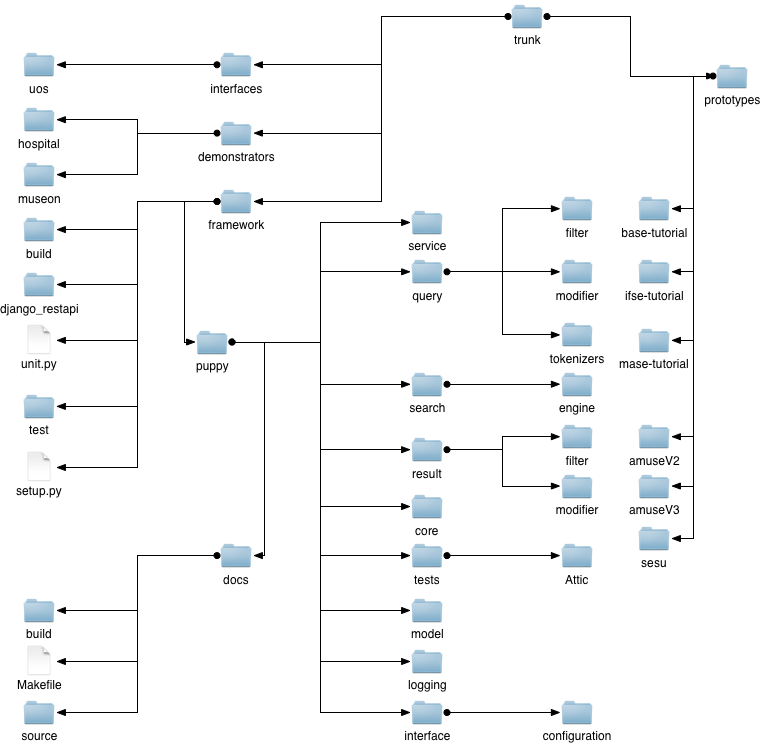
\includegraphics{trunk.png}
\caption{\emph{Diagram showing the structure of the `trunk' folder in the repository.}}\end{figure}


\subsubsection{Framework}
\label{repo:framework}
This folder contains the latest version of the framework, the test suite and the documentation (both the source and `compiled' versions). The main sections of this part are summarised below in terms of their contents (see {\hyperref[service:service-architecture]{\emph{Paradigm 1 - One Pipeline, One Search Engine}}} for a conceptual description from the perspective of a search service based architecture):
\begin{itemize}
\item {} 
\textbf{build} and \textbf{setup.py}: are the build directory (for when installing the framework) and the Python script to install the framework.

\item {} \begin{description}
\item[{\textbf{puppy}: the framework itself, its components are detailed below.}] \leavevmode\begin{itemize}
\item {} 
\textbf{core}: contains a type checking system and also various components for running threads.

\item {} 
\textbf{docs}: the documentation for the framework, including the source and compiled versions in addition to a make file to build the source.

\item {} 
\textbf{interface}: contains an early version of a Django application for configuring a search service.

\item {} 
\textbf{logging}: contains the query and event loggers.

\item {} 
\textbf{misc}: contains assorted files regarding aspects like stylistic conventions for code in the framework.

\item {} 
\textbf{model}: contains all the classes associated with the OpenSearch standard.

\item {} 
\textbf{query}: contains all the filters and modifiers belonging to the query pipeline in addition to the associated exceptions. It also contains various query tokenizers.

\item {} 
\textbf{result}: contains all the filters and modifiers belonging to the result pipeline in addition to the associated exceptions.

\item {} 
\textbf{search}: contains all the search engine wrappers and associated exceptions.

\item {} 
\textbf{service}: contains the service manager and search service classes. It also contains early work on configurable versions of the aforementioned, but, since these are tied into Django - they are not automatically imported by the framework.

\item {} 
\textbf{tests}: an old legacy version of the test suite; the new version is detailed below and supersedes this one.

\end{itemize}

\end{description}

\item {} 
\textbf{test} and \textbf{unit.py}: contains the test suite directory and the Python script for running the tests, please see: {\hyperref[test-suite:the-puppyir-framework-test-suite]{\emph{The PuppyIR Framework Test Suite}}} for details of this component.

\end{itemize}


\subsection{Trunk/Demonstrators}
\label{repo:trunk-demonstrators}
In the trunk there are two demonstrators which serve as showcases for the PuppyIR project; these demonstrators are described below.


\subsubsection{Hospital Demonstrator}
\label{repo:hospital-demonstrator}
This demonstrator, also known as the Emma Search service (EmSe), is being built for Emma Kinderziekenhuis (EKZ), which is part of the Amsterdam
Medical Centre (AMC). At the EKZ, children have access to a dedicated information centre as well as a dedicated bedside terminal. A user study carried out by hospital staff from the information centre has uncovered that children are reluctant to engage with the physical information centre (depending instead upon a family member or carer) and so, EmSe is designed to make use of these bedside terminals to allow them to access this resource via the web.

The motivators behind this demonstrator are, therefore, to:
\begin{enumerate}
\item {} 
improve knowledge of existence and possibilities of the information centre;

\item {} 
improve the accessibility of the information centre and its content for children;

\item {} 
expand the information content with reference to more extensive information on the internet that is both appropriate and suitable for the various development stages of the children.

\end{enumerate}

EmSe assists the children by providing appropriate query suggestions, simplifying difficult content and filtering unsuitable content based on age appropriateness.
\begin{figure}[htbp]
\centering
\capstart


\includegraphics{puppy-emse.png}
\caption{\emph{EmSe in action showing results from all the services; the dog's speech bubble is a query suggestion with the thought bubble containing more suggestions.}}\end{figure}


\subsubsection{Musueon Demonstrator}
\label{repo:musueon-demonstrator}
The Museum Demonstrator creates an interactive museum visit using advanced  technologies such as multitouch tables and marker tracking, creating the basis for additional data retrieval and filtering using the PuppyIR framework. Up to four users can use a multitouch table simultaneously to browse through the different exhibition subjects and together they determine the contents of an interactive quest.

Subsequently in a trail through the exhibitions users/players answer questions related to the chosen topics that have to be found. Throughout the museum various touch-screens equipped with scanners for reading and identifying the players are installed that when
triggered present the questions and provide feedback to answers.

After all questions have been answered, the multitouch table provides further information about the visited exhibits.
\begin{figure}[htbp]
\centering
\capstart

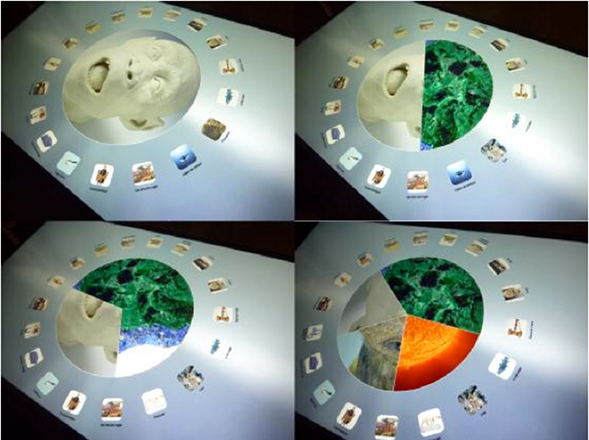
\includegraphics{puppy-musueon.png}
\caption{\emph{The Musueon demonstrator being used on multitouch tables; showing various topics.}}\end{figure}

You can view a video of this demonstrator in action by visiting: \href{http://www.youtube.com/watch?v=b5zycfgqlKo}{http://www.youtube.com/watch?v=b5zycfgqlKo}


\subsubsection{Prototypes}
\label{repo:prototypes}
This folder contains prototypes made using the latest version of the framework. These prototypes are either completed or in the late stages of development and so are all in a demonstrable state.

These prototypes are explained in: {\hyperref[prototypes:prototypes]{\emph{Running Prototypes}}} - please consult this page for more details.


\subsubsection{Interfaces}
\label{repo:interfaces}
This folder contains the University of Strathclyde's experimental environment on collaborative search interfaces.


\subsection{Branches}
\label{repo:branches}
This folder contains standalone components and unfinished/work-in-progress prototypes.
\begin{figure}[htbp]
\centering
\capstart

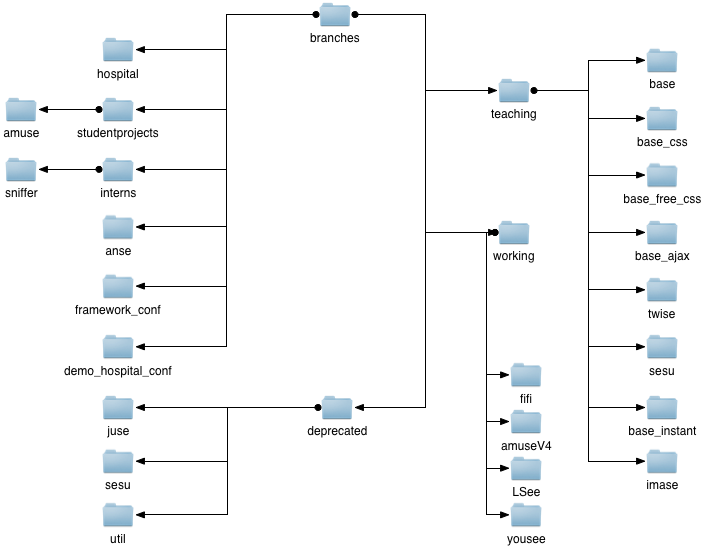
\includegraphics{branches.png}
\caption{\emph{Diagram showing the structure of the `branches' folder in the repository.}}\end{figure}

Branches contains:
\begin{itemize}
\item {} 
\textbf{AnSe} this is an application that uses the PuppyIR framework to query, using the Bing and YouTube wrappers, and retrieve results in the JSON format. It is totally standalone as it contains its own, reduced, local copy of the PuppyIR framework.

\item {} 
\textbf{conf demos (framework and hospital)} these are early versions of a method to allow for easy configuration of these resources.

\item {} 
\textbf{Interns}: a application called `sniffer' created by student interns working on PuppyIR, this application consists of: a search application similar to BaSe (see below for more on BaSe) and an automated logging application called ALF (Automated Logging Facility).

\item {} 
\textbf{Student projects} this contains applications made by students studying the \emph{Internet Technology} module at the University of Glasgow. At present it only contains the original version of the aMuSe application (the new versions, as detailed earlier, can be found in trunk) using an old version of the PuppyIR framework.

\item {} \begin{description}
\item[{\textbf{Teaching}: this folder contains various applications created (using the PuppyIR framework) as part of the \emph{Internet Technology} course at the University of Glasgow to teach students about web development. The individual applications it includes are:}] \leavevmode\begin{itemize}
\item {} 
\textbf{BaSe}: a basic search engine that searches for and display web results.

\item {} 
\textbf{BaSe CSS}: same as BaSe but with CSS styling applied to it.

\item {} 
\textbf{BaSe Free CSS}: same as BaSe but with multiple different styles available and style switching code (in JavaScript).

\item {} 
\textbf{BaSe Ajax}: same as BaSe but it searches for, retrieves and displays web results using Ajax.

\item {} 
\textbf{BaSe Instant}: same as above but using code from a live in-lecture demo - no major differences to BaSe Ajax.

\item {} 
\textbf{TwiSe}: a basic twitter search engine for finding and displaying tweets.

\item {} 
\textbf{SeSu}: another alternate version of the now deprecated SeSu prototype.

\item {} 
\textbf{ImaSe}: a basic image search engine for finding and displaying images.

\end{itemize}

\end{description}

\item {} \begin{description}
\item[{\textbf{Working}: this folder contains prototypes that, while using the latest version of the framework, are still work-in-progress. These prototypes are described at the end of the `branches' section.}] \leavevmode\begin{itemize}
\item {} 
\textbf{Deprecated}: these prototypes use an outdated local version of the framework (called `util'). SeSu does not work anymore but JuSe does still function. Both applications and `util' are no longer supported (however, SeSu has been remade and can be found in the `trunk').

\end{itemize}

\end{description}

\end{itemize}


\subsubsection{Work-in-progress prototypes}
\label{repo:work-in-progress-prototypes}
There are several prototypes contained within the aforementioned `working' folder. These prototypes provide further examples of how to use the framework but remain in-complete and as such, may contain flaws and/or not fully function.
\begin{itemize}
\item {} 
\textbf{aMuSeV4}: an application based around children retrieving image results and using these to create stories in a comic book style format. This application is, currently, very incomplete.

\item {} 
\textbf{FiFi}: this folder is a placeholder for an application deployed on a server at Glasgow - \href{http://pooley.dcs.gla.ac.uk:8080/fifi/}{http://pooley.dcs.gla.ac.uk:8080/fifi/}

\item {} 
\textbf{LSee}: an application allowing children to search for a location and, from this location, retrieve a mash-up of search results (image, video, tweets and news) taken from that location. LSee (Location Search) is, functionality wise, fairly well developed but the layout and styling is very basic.

\item {} 
\textbf{YouSee}: YouSee is a web application designed to provide a fun, safe, environment for children to browse videos. Videos are presented in the form of carousels. Each carousel represents a category and contains a series of videos related to it. A child using YouSee can, watch a video and browse videos in the current carousel or change to a different one. Carousels are created for the children by their parent/guardian. This application is functionally almost complete but, interaction wise, the carousel browsing is in-complete - existing only in a temporary static form.

\end{itemize}

N.B. Once completed, these prototypes will be moved to \textbf{`trunk/prototypes'}.


\subsection{Tags}
\label{repo:tags}
This folder contains archived versions of the Hospital demonstrator (EmSe/Emma Search), the framework and the teaching applications (found in branches). These will only be of interest with respect to the evolution of the various parts and/or in the event of having to revert to a older version - for whatever reason.
\begin{figure}[htbp]
\centering
\capstart

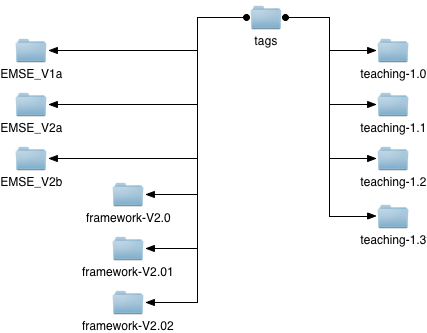
\includegraphics{tag.png}
\caption{\emph{Diagram showing the structure of the `tags' folder in the repository.}}\end{figure}


\section{Known issues with the PuppyIR framework}
\label{issues:known-issues-with-the-puppyir-framework}\label{issues::doc}\label{issues:issues}
This section details known issues with the PuppyIR framework and will be kept up-to-date as new versions of the framework are released.


\subsection{Python 2.6 issues}
\label{issues:python-2-6-issues}
In the {\hyperref[overview:overview]{\emph{Overview and background of the PuppyIR Framework}}} section it is noted that the framework is intended to be used with Python 2.7. The use of Python 2.6 has not been tested thoroughly and as such the list below of issues with it is not comprehensive (it is still recommenced to switch to Python 2.7 to avoid these and other potential problems):
\begin{itemize}
\item {} 
aMuSeV3 does not work due to a change to the `fractions' library between Python 2.6 and Python 2.7 regarding the valid format(s) of data it can handle.

\item {} 
Both the YouTube and YouTubeV2 wrappers function, but lose all details of thumbnails in Python 2.6 due to a change in how Atom/Xml feeds are parsed.

\end{itemize}


\chapter{API Reference}
\label{index:api-reference}

\section{PuppyIR API Reference}
\label{api2.0:api}\label{api2.0::doc}\label{api2.0:puppyir-api-reference}

\subsection{puppy.service}
\label{api2.0:puppy-service}
This module contains classes for building a service.
\phantomsection\label{api2.0:module-puppy.service}\index{puppy.service (module)}

\subsubsection{ServiceManager}
\label{api2.0:servicemanager}\index{ServiceManager (class in puppy.service)}

\begin{fulllineitems}
\phantomsection\label{api2.0:puppy.service.ServiceManager}\pysiglinewithargsret{\strong{class }\code{puppy.service.}\bfcode{ServiceManager}}{\emph{config}}{}
Manages a collection of search services for a PuppyIR Service
\index{add\_search\_service() (puppy.service.ServiceManager method)}

\begin{fulllineitems}
\phantomsection\label{api2.0:puppy.service.ServiceManager.add_search_service}\pysiglinewithargsret{\bfcode{add\_search\_service}}{\emph{obj}}{}
Add a search service

\end{fulllineitems}

\index{remove\_search\_service() (puppy.service.ServiceManager method)}

\begin{fulllineitems}
\phantomsection\label{api2.0:puppy.service.ServiceManager.remove_search_service}\pysiglinewithargsret{\bfcode{remove\_search\_service}}{\emph{service\_or\_name}}{}
Removes an exisiting search service

\end{fulllineitems}


\end{fulllineitems}



\subsubsection{SearchService}
\label{api2.0:searchservice}\index{SearchService (class in puppy.service)}

\begin{fulllineitems}
\phantomsection\label{api2.0:puppy.service.SearchService}\pysiglinewithargsret{\strong{class }\code{puppy.service.}\bfcode{SearchService}}{\emph{service\_manager}, \emph{name}}{}
Models the configuration of a QueryFilter pipeline, Search Engine, and a ResultFilter pipeline.
\index{add\_filters() (puppy.service.SearchService method)}

\begin{fulllineitems}
\phantomsection\label{api2.0:puppy.service.SearchService.add_filters}\pysiglinewithargsret{\bfcode{add\_filters}}{\emph{*filters}}{}
Add one or more filters. Detects filter type (e.g., QueryFilter,
ResultModifier) and places in appropriate pipeline.

\end{fulllineitems}

\index{add\_query\_filter() (puppy.service.SearchService method)}

\begin{fulllineitems}
\phantomsection\label{api2.0:puppy.service.SearchService.add_query_filter}\pysiglinewithargsret{\bfcode{add\_query\_filter}}{\emph{query\_filter}}{}
Add filter to query filter pipeline.

\end{fulllineitems}

\index{add\_query\_modifier() (puppy.service.SearchService method)}

\begin{fulllineitems}
\phantomsection\label{api2.0:puppy.service.SearchService.add_query_modifier}\pysiglinewithargsret{\bfcode{add\_query\_modifier}}{\emph{query\_modifier}}{}
Add modifier to query modifier pipeline.

\end{fulllineitems}

\index{add\_result\_filter() (puppy.service.SearchService method)}

\begin{fulllineitems}
\phantomsection\label{api2.0:puppy.service.SearchService.add_result_filter}\pysiglinewithargsret{\bfcode{add\_result\_filter}}{\emph{result\_filter}}{}
Add filter to result filter pipeline.

\end{fulllineitems}

\index{add\_result\_modifier() (puppy.service.SearchService method)}

\begin{fulllineitems}
\phantomsection\label{api2.0:puppy.service.SearchService.add_result_modifier}\pysiglinewithargsret{\bfcode{add\_result\_modifier}}{\emph{result\_modifier}}{}
Add filter to result filter pipeline.

\end{fulllineitems}

\index{clear\_filters() (puppy.service.SearchService method)}

\begin{fulllineitems}
\phantomsection\label{api2.0:puppy.service.SearchService.clear_filters}\pysiglinewithargsret{\bfcode{clear\_filters}}{}{}
Remove all existing filters.

\end{fulllineitems}

\index{replace\_filters() (puppy.service.SearchService method)}

\begin{fulllineitems}
\phantomsection\label{api2.0:puppy.service.SearchService.replace_filters}\pysiglinewithargsret{\bfcode{replace\_filters}}{\emph{*filters}}{}
Replace existing filters with new filters.

\end{fulllineitems}

\index{search() (puppy.service.SearchService method)}

\begin{fulllineitems}
\phantomsection\label{api2.0:puppy.service.SearchService.search}\pysiglinewithargsret{\bfcode{search}}{\emph{query}, \emph{offset=0}, \emph{highlight=False}}{}
Search with query and result filter pipelines active.

Parameters:
\begin{itemize}
\item {} 
query (puppy.model.Query): search query

\item {} 
offset (int): result offset

\end{itemize}

Returns:
\begin{itemize}
\item {} 
results (puppy.model.Response): search results

\end{itemize}

\end{fulllineitems}

\index{simplesearch() (puppy.service.SearchService method)}

\begin{fulllineitems}
\phantomsection\label{api2.0:puppy.service.SearchService.simplesearch}\pysiglinewithargsret{\bfcode{simplesearch}}{\emph{query}, \emph{offset=0}}{}
Search without query and result filter pipelines.

Parameters:
\begin{itemize}
\item {} 
query (puppy.model.Query): search query

\item {} 
offset (int): result offset

\end{itemize}

Returns:
\begin{itemize}
\item {} 
results (puppy.model.Response): search results

\end{itemize}

\end{fulllineitems}


\end{fulllineitems}



\subsection{puppy.pipeline}
\label{api2.0:module-puppy.pipeline}\label{api2.0:puppy-pipeline}\index{puppy.pipeline (module)}
This module contains an alternate paradigm for creating a PuppyIR based service, where you construct one Pipeline, store multiple search engines and then either: search all or, search a specific one using the Pipeline. See: {\hyperref[pipeline:pipeline-architecture]{\emph{Paradigm 2 - One Pipeline, Many Search Engines}}} for an explanation of this paradigm and {\hyperref[pipeline-tutorial:pipeline-puppyir-tutorial]{\emph{Pipeline Tutorial: DeeSe (Detective Search)}}} for details about how to go about using it to create an application.


\subsubsection{PipelineService}
\label{api2.0:pipelineservice}\index{PipelineService (class in puppy.pipeline)}

\begin{fulllineitems}
\phantomsection\label{api2.0:puppy.pipeline.PipelineService}\pysiglinewithargsret{\strong{class }\code{puppy.pipeline.}\bfcode{PipelineService}}{\emph{config}, \emph{name}}{}
Models the configuration of a Pipeline (QueryFilters/Modifiers and ResultFilters/Modifiers) and the search engines using the Pipeline
\index{add\_filters() (puppy.pipeline.PipelineService method)}

\begin{fulllineitems}
\phantomsection\label{api2.0:puppy.pipeline.PipelineService.add_filters}\pysiglinewithargsret{\bfcode{add\_filters}}{\emph{*filters}}{}
Add one or more filters. Detects filter type (e.g., QueryFilter, ResultModifier) and places in appropriate pipeline.

\end{fulllineitems}

\index{add\_query\_filter() (puppy.pipeline.PipelineService method)}

\begin{fulllineitems}
\phantomsection\label{api2.0:puppy.pipeline.PipelineService.add_query_filter}\pysiglinewithargsret{\bfcode{add\_query\_filter}}{\emph{query\_filter}}{}
Add filter to query filter pipeline.

\end{fulllineitems}

\index{add\_query\_modifier() (puppy.pipeline.PipelineService method)}

\begin{fulllineitems}
\phantomsection\label{api2.0:puppy.pipeline.PipelineService.add_query_modifier}\pysiglinewithargsret{\bfcode{add\_query\_modifier}}{\emph{query\_modifier}}{}
Add modifier to query modifier pipeline.

\end{fulllineitems}

\index{add\_result\_filter() (puppy.pipeline.PipelineService method)}

\begin{fulllineitems}
\phantomsection\label{api2.0:puppy.pipeline.PipelineService.add_result_filter}\pysiglinewithargsret{\bfcode{add\_result\_filter}}{\emph{result\_filter}}{}
Add filter to result filter pipeline.

\end{fulllineitems}

\index{add\_result\_modifier() (puppy.pipeline.PipelineService method)}

\begin{fulllineitems}
\phantomsection\label{api2.0:puppy.pipeline.PipelineService.add_result_modifier}\pysiglinewithargsret{\bfcode{add\_result\_modifier}}{\emph{result\_modifier}}{}
Add filter to result filter pipeline.

\end{fulllineitems}

\index{clear\_filters() (puppy.pipeline.PipelineService method)}

\begin{fulllineitems}
\phantomsection\label{api2.0:puppy.pipeline.PipelineService.clear_filters}\pysiglinewithargsret{\bfcode{clear\_filters}}{}{}
Remove all existing filters.

\end{fulllineitems}

\index{replace\_filters() (puppy.pipeline.PipelineService method)}

\begin{fulllineitems}
\phantomsection\label{api2.0:puppy.pipeline.PipelineService.replace_filters}\pysiglinewithargsret{\bfcode{replace\_filters}}{\emph{*filters}}{}
Replace existing filters with new filters.

\end{fulllineitems}

\index{searchAll() (puppy.pipeline.PipelineService method)}

\begin{fulllineitems}
\phantomsection\label{api2.0:puppy.pipeline.PipelineService.searchAll}\pysiglinewithargsret{\bfcode{searchAll}}{\emph{query}, \emph{offset=0}}{}
Search all the search engines currently stored by our `SearchEngineManager' using the query and result pipeline as currently defined.

Parameters:
\begin{itemize}
\item {} 
query (puppy.model.Query): search query

\item {} 
offset (int): result offset

\end{itemize}

Returns:
\begin{itemize}
\item {} 
results\_dict (dictionary of puppy.model.Response): the key being the name of the search egine and the value the reponse object

\end{itemize}

\end{fulllineitems}

\index{searchSpecificEngine() (puppy.pipeline.PipelineService method)}

\begin{fulllineitems}
\phantomsection\label{api2.0:puppy.pipeline.PipelineService.searchSpecificEngine}\pysiglinewithargsret{\bfcode{searchSpecificEngine}}{\emph{query}, \emph{searchEngineName}, \emph{offset=0}}{}
Search a specific search engine only, if it's currently stored by our `SearchEngineManager' using the query and result pipeline as currently defined.

Parameters:
\begin{itemize}
\item {} 
query (puppy.model.Query): search query

\item {} 
searchEngineName (str): the name of the search engine to search which will be searched if it's currently stored

\item {} 
offset (int): result offset

\end{itemize}

Returns:
\begin{itemize}
\item {} 
results\_dict (dictionary of puppy.model.Response): the key being the name of the search egine and the value the reponse object

\end{itemize}

\end{fulllineitems}


\end{fulllineitems}



\subsubsection{SearchEngineManager}
\label{api2.0:searchenginemanager}\index{SearchEngineManager (class in puppy.pipeline)}

\begin{fulllineitems}
\phantomsection\label{api2.0:puppy.pipeline.SearchEngineManager}\pysigline{\strong{class }\code{puppy.pipeline.}\bfcode{SearchEngineManager}}
Manages a collection of search engines the Pipeline Manager can act upon
\index{add\_search\_engine() (puppy.pipeline.SearchEngineManager method)}

\begin{fulllineitems}
\phantomsection\label{api2.0:puppy.pipeline.SearchEngineManager.add_search_engine}\pysiglinewithargsret{\bfcode{add\_search\_engine}}{\emph{search\_engine\_name}, \emph{search\_engine}}{}
Adds a search engine to the Pipeline Manager if it's valid and not already stored by the Manager

\end{fulllineitems}

\index{clear\_search\_engines() (puppy.pipeline.SearchEngineManager method)}

\begin{fulllineitems}
\phantomsection\label{api2.0:puppy.pipeline.SearchEngineManager.clear_search_engines}\pysiglinewithargsret{\bfcode{clear\_search\_engines}}{}{}
Remove all existing search engines.

\end{fulllineitems}

\index{get\_search\_engine() (puppy.pipeline.SearchEngineManager method)}

\begin{fulllineitems}
\phantomsection\label{api2.0:puppy.pipeline.SearchEngineManager.get_search_engine}\pysiglinewithargsret{\bfcode{get\_search\_engine}}{\emph{search\_engine\_name}}{}
If the specified search engine is stored return it, otherwise, return None

\end{fulllineitems}

\index{get\_search\_engines() (puppy.pipeline.SearchEngineManager method)}

\begin{fulllineitems}
\phantomsection\label{api2.0:puppy.pipeline.SearchEngineManager.get_search_engines}\pysiglinewithargsret{\bfcode{get\_search\_engines}}{}{}
Return all the currently stored search engines

\end{fulllineitems}

\index{remove\_search\_engine() (puppy.pipeline.SearchEngineManager method)}

\begin{fulllineitems}
\phantomsection\label{api2.0:puppy.pipeline.SearchEngineManager.remove_search_engine}\pysiglinewithargsret{\bfcode{remove\_search\_engine}}{\emph{search\_engine\_name}}{}
Removed a search engine from the Pipeline Manager if it's currently stored by the Manager

\end{fulllineitems}


\end{fulllineitems}



\subsection{puppy.search}
\label{api2.0:module-puppy.search}\label{api2.0:puppy-search}\index{puppy.search (module)}

\subsubsection{SearchEngine}
\label{api2.0:searchengine}\index{SearchEngine (class in puppy.search)}

\begin{fulllineitems}
\phantomsection\label{api2.0:puppy.search.SearchEngine}\pysiglinewithargsret{\strong{class }\code{puppy.search.}\bfcode{SearchEngine}}{\emph{service}, \emph{**args}}{}
Abstract search engine interface.
\index{configure\_opener() (puppy.search.SearchEngine method)}

\begin{fulllineitems}
\phantomsection\label{api2.0:puppy.search.SearchEngine.configure_opener}\pysiglinewithargsret{\bfcode{configure\_opener}}{}{}
Configure urllib2 opener with network proxy

\end{fulllineitems}

\index{search() (puppy.search.SearchEngine method)}

\begin{fulllineitems}
\phantomsection\label{api2.0:puppy.search.SearchEngine.search}\pysiglinewithargsret{\bfcode{search}}{\emph{query}, \emph{pos=1}}{}
Perform a search.

Parameters:
\begin{itemize}
\item {} 
query (puppy.model.Query): query object

\item {} 
pos (int): result offset

\end{itemize}

Returns:
\begin{itemize}
\item {} 
results (puppy.model.Response): results of the search

\end{itemize}

\end{fulllineitems}


\end{fulllineitems}



\subsection{puppy.search.exceptions}
\label{api2.0:module-puppy.search.exceptions}\label{api2.0:puppy-search-exceptions}\index{puppy.search.exceptions (module)}

\subsubsection{SearchEngineError}
\label{api2.0:searchengineerror}\index{SearchEngineError (class in puppy.search.exceptions)}

\begin{fulllineitems}
\phantomsection\label{api2.0:puppy.search.exceptions.SearchEngineError}\pysiglinewithargsret{\strong{class }\code{puppy.search.exceptions.}\bfcode{SearchEngineError}}{\emph{searchEngineName}, \emph{error}, \emph{**extras}}{}
Use for exceptions in which the search engine wrapper fails - this can be for multiple reasons, 
for example: the lack of a proxy server in config or a search service being down. Callers should respond
to this in a way that fails gracefully.

\end{fulllineitems}



\subsubsection{ApiKeyError}
\label{api2.0:apikeyerror}\index{ApiKeyError (class in puppy.search.exceptions)}

\begin{fulllineitems}
\phantomsection\label{api2.0:puppy.search.exceptions.ApiKeyError}\pysiglinewithargsret{\strong{class }\code{puppy.search.exceptions.}\bfcode{ApiKeyError}}{\emph{searchEngineName}, \emph{apiFieldName}}{}
Use for exceptions in which the API for a wrapper, which requires one, has not been supplied. Callers should
respond in such a way that the developer, it is not intended for users of an application, are aware of the issue
and so can take the necessary steps to rectify the issue.

\end{fulllineitems}



\subsection{puppy.search.engine}
\label{api2.0:puppy-search-engine}\label{api2.0:module-puppy.search.engine}\index{puppy.search.engine (module)}

\subsubsection{Bing}
\label{api2.0:bing}\index{Bing (class in puppy.search.engine)}

\begin{fulllineitems}
\phantomsection\label{api2.0:puppy.search.engine.Bing}\pysiglinewithargsret{\strong{class }\code{puppy.search.engine.}\bfcode{Bing}}{\emph{service}, \emph{site=None}, \emph{source='web'}, \emph{adult='Strict'}, \emph{market='en-GB'}, \emph{resultsPerPage=10}, \emph{lat=None}, \emph{lon=None}, \emph{radius=5}, \emph{sites=None}, \emph{**args}}{}
Bing search engine wrapper.

Note: you can only use location based searching with sourcetypes `web' and `phonebook'; however, with web, it doesn't appear to have any effect

Parameters:
\begin{itemize}
\item {} 
site: if you wish to search specific websites for results

\item {} 
source (str): web, image, news are the options

\item {} 
adult (str): strict, i.e. safesearch not recommended to change from the default

\item {} 
market (str): i.e. which area's results are prioritised more - en-gb is the UK

\item {} 
resultsPerPage (int): How many results per page

\item {} 
lat (double): the latitude of the place you want to search in

\item {} 
lon (double): the longitude of the place you want to search in

\item {} 
radius (int): the radius to retrieve results from around lat and lon; 0-250miles is the limit

\end{itemize}

\end{fulllineitems}



\subsubsection{BingSite}
\label{api2.0:bingsite}\index{BingSite (class in puppy.search.engine)}

\begin{fulllineitems}
\phantomsection\label{api2.0:puppy.search.engine.BingSite}\pysiglinewithargsret{\strong{class }\code{puppy.search.engine.}\bfcode{BingSite}}{\emph{service}, \emph{site=None}, \emph{source='web'}}{}
Bing site search engine wrapper.

Parameters:
\begin{itemize}
\item {} 
site: if you wish to search specific websites for results

\item {} 
source (str): web, image, news are the options

\end{itemize}

\end{fulllineitems}



\subsubsection{BingV2 (API Version 2.2)}
\label{api2.0:bingv2-api-version-2-2}\index{BingV2 (class in puppy.search.engine)}

\begin{fulllineitems}
\phantomsection\label{api2.0:puppy.search.engine.BingV2}\pysiglinewithargsret{\strong{class }\code{puppy.search.engine.}\bfcode{BingV2}}{\emph{service}, \emph{source='Web'}, \emph{adult='Strict'}, \emph{market='en-GB'}, \emph{resultsPerPage=8}, \emph{filters=None}, \emph{sortBy=None}, \emph{newsCategory=None}, \emph{sites=None}, \emph{**args}}{}
Bing search engine wrapper for Version 2.X of the API - allowing for News, Web, Image and Video results to be retrieved

One of the key advantages of using this wrapper is using the new features and also being able to use multiple sources to create a mash-up.
i.e. source=''Web+Image'' gets results from the web and also image search services.

You must include your application's Bing ID in your service manage config to use this service. It should be under the identifier ``bing\_api\_key''

If you are using the `Spell' then you must set the `market' parameter to match the language you are querying in i.e. English UK set Market to en-gb or Dutch set it to nl-nl

Parameters:
\begin{itemize}
\item {} 
source (str): what source the results should come from, valid options are: Web, News, Video, Image, Spell, RelatedSearch.

\item {} 
adult (str):  Strict is the default, not recommended to change this

\item {} 
market (str): For UK: en-GB, For Netherlands: nl-NL etc

\item {} 
resultsPerPage (int): How many results per page

\end{itemize}

-- Image and Video Only Parameters --
\begin{itemize}
\item {} 
filters (str): filter options split up by `+' you can only have one of each type see Bing API documentation for what these are

\end{itemize}

-- Video and News Only Paramters --
\begin{itemize}
\item {} 
sortBy (str): sort news by either `Date' or `Relevance'

\end{itemize}

-- News Only Parameters --
\begin{itemize}
\item {} 
newsCategory (str): what sort of news is wanted - see BingAPI for list of options, for example: `rt\_ScienceAndTechnology'

\end{itemize}

\end{fulllineitems}



\subsubsection{Digg}
\label{api2.0:digg}\index{Digg (class in puppy.search.engine)}

\begin{fulllineitems}
\phantomsection\label{api2.0:puppy.search.engine.Digg}\pysiglinewithargsret{\strong{class }\code{puppy.search.engine.}\bfcode{Digg}}{\emph{service}, \emph{resultsPerPage=8}, \emph{sort=None}, \emph{topic=None}, \emph{media='all'}, \emph{max\_date=None}, \emph{min\_date=None}, \emph{**args}}{}
Digg search engine wrapper.

Parameters:
\begin{itemize}
\item {} 
resultsPerPage (int): How many results per page

\item {} 
sort (str): how to sort results (see Digg site for a list of the options) an example is `submit\_date-desc' to sort via the item's submit date

\item {} 
topic (str): restrict the search to a specific topic (see Digg site for a list of them)

\item {} 
media (str): options are: `all', `news', `videos', `images'

\item {} 
max\_date (unix timestamp - converted to str): latest date results returned were posted

\item {} 
min\_date (unix timestamp - converted to str): earliest date results returned were posted

\end{itemize}

\end{fulllineitems}



\subsubsection{EmmaSearch}
\label{api2.0:emmasearch}\index{EmmaSearch (class in puppy.search.engine)}

\begin{fulllineitems}
\phantomsection\label{api2.0:puppy.search.engine.EmmaSearch}\pysiglinewithargsret{\strong{class }\code{puppy.search.engine.}\bfcode{EmmaSearch}}{\emph{service}, \emph{age='v'}, \emph{resultsPerPage=10}, \emph{**args}}{}
EmmaSearch search engine.

Parameters:
\begin{itemize}
\item {} 
age (str): values - `v' for adults (shows all `a' and `k' results too), `a' for teenagers, and `k' for children

\item {} 
resultsPerPage (int): How many results per page - the default for the emma search service is 10

\end{itemize}

\end{fulllineitems}



\subsubsection{EmmaSearch SQL Server version}
\label{api2.0:emmasearch-sql-server-version}
A new version of the above (EmmaSearch) wrapper allowing for searching the Emma Hospital database using a Microsoft's SQL server.

Due to this SQL Server import being an extra (see the installation section for details about installing it), rather than required, you cannot import this wrapper from `\emph{puppy.search.engine}` like the above wrappers; you import them using the code below:

\begin{Verbatim}[commandchars=\\\{\}]
\PYG{k+kn}{from} \PYG{n+nn}{puppy.search.engine.emmasearchMSSQL} \PYG{k+kn}{import} \PYG{n}{EmmaSearchMSSQL}
\end{Verbatim}


\subsubsection{Flickr}
\label{api2.0:flickr}\index{Flickr (class in puppy.search.engine)}

\begin{fulllineitems}
\phantomsection\label{api2.0:puppy.search.engine.Flickr}\pysiglinewithargsret{\strong{class }\code{puppy.search.engine.}\bfcode{Flickr}}{\emph{service}, \emph{sortBy='relevance'}, \emph{safeSearch=3}, \emph{mediaType='photos'}, \emph{resultsPerPage=8}, \emph{bbox=None}, \emph{**args}}{}
Flickr search engine.

You must include your application's Flickr ID in your service manage config to use this service
it should be under the identifier ``flickr\_api\_key''

Parameters:
\begin{itemize}
\item {} 
sortBy (str):  how we sort results, default is relevance see Flickr API for more details

\item {} 
safeSearch (int): default is 3, i.e. strict, not recommended to change this

\item {} 
mediaType (str): all, photos, videos are the options

\item {} 
resultsPerPage (int): How many results per page

\item {} 
bbox (str): replace the names with the values of the corners of the bounding box `swLongitude,swLatitude,neLongitude,neLatitude'

\end{itemize}

\end{fulllineitems}



\subsubsection{Google Geocode}
\label{api2.0:google-geocode}\index{GoogleGeocode (class in puppy.search.engine)}

\begin{fulllineitems}
\phantomsection\label{api2.0:puppy.search.engine.GoogleGeocode}\pysiglinewithargsret{\strong{class }\code{puppy.search.engine.}\bfcode{GoogleGeocode}}{\emph{service}, \emph{sensor='false'}, \emph{**args}}{}
GoogleGeocode search service.

Parameters:
\begin{itemize}
\item {} 
sensor(str): does your device have a GPS sensor or not, not recommended to change from `false' but the other option is, naturally, `true' - must be lowercase

\end{itemize}

\end{fulllineitems}



\subsubsection{Google (depreciated)}
\label{api2.0:google-depreciated}\index{Google (class in puppy.search.engine)}

\begin{fulllineitems}
\phantomsection\label{api2.0:puppy.search.engine.Google}\pysiglinewithargsret{\strong{class }\code{puppy.search.engine.}\bfcode{Google}}{\emph{service}, \emph{**args}}{}
Google search engine.

Google have regrettfully retired this search api

Code is left here for reference purposes

\end{fulllineitems}



\subsubsection{Google Books}
\label{api2.0:google-books}\index{GoogleBooks (class in puppy.search.engine)}

\begin{fulllineitems}
\phantomsection\label{api2.0:puppy.search.engine.GoogleBooks}\pysiglinewithargsret{\strong{class }\code{puppy.search.engine.}\bfcode{GoogleBooks}}{\emph{service}, \emph{resultsPerPage=8}, \emph{langRestrict=None}, \emph{filter=None}, \emph{orderBy='relevance'}, \emph{printType=None}, \emph{**args}}{}
Google's Books search engine api.

See documentation for how to specify advanced queries i.e. Hobbit+inauthor:Tolkien

Parameters:
\begin{itemize}
\item {} 
resultsPerPage (int): How many results per page

\item {} 
langRestrict (str): restrict results to a certain language i.e. `en' for English

\item {} 
filter (str): filter volumes by type/availabilty, valid values - `partial', `full', `free-ebooks', `paid-ebooks', `ebooks'

\item {} 
orderBy (str): order either by `relevance' or `newest'

\item {} 
printType (str): `all', `books' or `magazines' restrict the results to either all or one of the preceding types of media only

\end{itemize}

\end{fulllineitems}



\subsubsection{Guardian}
\label{api2.0:guardian}\index{Guardian (class in puppy.search.engine)}

\begin{fulllineitems}
\phantomsection\label{api2.0:puppy.search.engine.Guardian}\pysiglinewithargsret{\strong{class }\code{puppy.search.engine.}\bfcode{Guardian}}{\emph{service}, \emph{orderBy='newest'}, \emph{**args}}{}
Guardian search engine.

Warning: `StandFirst' is the result field used for description; it is a form of abstract for the news story.
It can however, contain html tags and so when processing these results outside the framework care needs to be
taken.

Parameters:
\begin{itemize}
\item {} 
orderBy (str): the options are - `newest', `oldest' and `relevance'

\end{itemize}

\end{fulllineitems}



\subsubsection{iTunes}
\label{api2.0:itunes}\index{ITunes (class in puppy.search.engine)}

\begin{fulllineitems}
\phantomsection\label{api2.0:puppy.search.engine.ITunes}\pysiglinewithargsret{\strong{class }\code{puppy.search.engine.}\bfcode{ITunes}}{\emph{service}, \emph{country='gb'}, \emph{lang='en\_gb'}, \emph{media=None}, \emph{resultsPerPage=8}, \emph{explicit=False}, \emph{**args}}{}
iTunes search engine wrapper - allowing for Track, Album and Artist search results to be retrieved

If you change either lang or country change the other variable to match i.e. change lang to `en\_gb' you should also change
country to `gb' to match or vice-versa.

Parameters:
\begin{itemize}
\item {} 
country (str): Which iTunes store to search i.e. `gb' for the UK and `us' for the USA etc

\item {} 
lang (str): the language the results should be returned in

\item {} 
media(str): the media type you want to search for (see iTunes documentation for others e.g. `movie' etc)

\item {} 
resultsPerPage (int): How many results per page

\item {} 
explicit (boolean): Do we want to return results marked as including explicit content (not recommended to change this)

\end{itemize}

\end{fulllineitems}



\subsubsection{LastFM}
\label{api2.0:lastfm}\index{LastFM (class in puppy.search.engine)}

\begin{fulllineitems}
\phantomsection\label{api2.0:puppy.search.engine.LastFM}\pysiglinewithargsret{\strong{class }\code{puppy.search.engine.}\bfcode{LastFM}}{\emph{service}, \emph{source='track'}, \emph{resultsPerPage=8}, \emph{artist=None}, \emph{**args}}{}
LastFM search engine wrapper - allowing for Track, Album and Artist search results to be retrieved

You must include your application's LastFM ID in your service manage config to use this service. It should be under the identifier ``last\_fm\_api\_key''

Parameters:
\begin{itemize}
\item {} 
source (str): What to search for, valid types: `track', `album' and `artist'

\item {} 
resultsPerPage (int): How many results per page

\end{itemize}

-- Track Only Parameters --
\begin{itemize}
\item {} 
artist (str): the artist for the tracks you are searching for

\end{itemize}

\end{fulllineitems}



\subsubsection{OpenSearch}
\label{api2.0:opensearch}\index{OpenSearch (class in puppy.search.engine)}

\begin{fulllineitems}
\phantomsection\label{api2.0:puppy.search.engine.OpenSearch}\pysiglinewithargsret{\strong{class }\code{puppy.search.engine.}\bfcode{OpenSearch}}{\emph{service}, \emph{url}, \emph{**args}}{}
OpenSearch search engine.

\end{fulllineitems}



\subsubsection{Picassa}
\label{api2.0:picassa}\index{Picassa (class in puppy.search.engine)}

\begin{fulllineitems}
\phantomsection\label{api2.0:puppy.search.engine.Picassa}\pysiglinewithargsret{\strong{class }\code{puppy.search.engine.}\bfcode{Picassa}}{\emph{service}, \emph{resultsPerPage=8}, \emph{access='public'}, \emph{kind='photo'}, \emph{**args}}{}
Picassa search engine.

Parameters:
\begin{itemize}
\item {} 
resultsPerPage (int): select how many results per page

\item {} 
access (str): public, private (it is not recommended to change to private), all, visible

\item {} 
kind (str): photo is the only working option

\end{itemize}

\end{fulllineitems}



\subsubsection{Rotten Tomatoes}
\label{api2.0:rotten-tomatoes}\index{RottenTomatoes (class in puppy.search.engine)}

\begin{fulllineitems}
\phantomsection\label{api2.0:puppy.search.engine.RottenTomatoes}\pysiglinewithargsret{\strong{class }\code{puppy.search.engine.}\bfcode{RottenTomatoes}}{\emph{service}, \emph{resultsPerPage=8}, \emph{**args}}{}
RottenTomatoes search engine.

You must include your application's Rotten Tomatoes ID in your service manage config to use this service
it should be under the identifier ``rotten\_tomatoes\_api\_key''

Parameters:
\begin{itemize}
\item {} 
resultsPerPage (int): How many results per page

\end{itemize}

\end{fulllineitems}



\subsubsection{SimpleWikipedia}
\label{api2.0:simplewikipedia}\index{SimpleWikipedia (class in puppy.search.engine)}

\begin{fulllineitems}
\phantomsection\label{api2.0:puppy.search.engine.SimpleWikipedia}\pysiglinewithargsret{\strong{class }\code{puppy.search.engine.}\bfcode{SimpleWikipedia}}{\emph{service}, \emph{resultsPerPage=8}, \emph{**args}}{}
Simple Wikipedia search engine.

Parameters:
\begin{itemize}
\item {} 
resultsPerPage (int): How many results per page - note with Wiki only one page of results is returned.

\end{itemize}

\end{fulllineitems}



\subsubsection{Solr}
\label{api2.0:solr}\index{Solr (class in puppy.search.engine)}

\begin{fulllineitems}
\phantomsection\label{api2.0:puppy.search.engine.Solr}\pysiglinewithargsret{\strong{class }\code{puppy.search.engine.}\bfcode{Solr}}{\emph{service}, \emph{url}, \emph{**args}}{}
Solr search engine.

\end{fulllineitems}



\subsubsection{SoundCloud}
\label{api2.0:soundcloud}\index{SoundCloud (class in puppy.search.engine)}

\begin{fulllineitems}
\phantomsection\label{api2.0:puppy.search.engine.SoundCloud}\pysiglinewithargsret{\strong{class }\code{puppy.search.engine.}\bfcode{SoundCloud}}{\emph{service}, \emph{resultsPerPage=8}, \emph{order=None}, \emph{tags=None}, \emph{filter=None}, \emph{genres=None}, \emph{types=None}, \emph{bpmFilter=None}, \emph{durationFilter=None}, \emph{createdFilter=None}, \emph{**args}}{}
SoundCliud search engine wrapper for a music sharing application allowing the searching for tracks.

You must include your api key for Wordnik in your service manage config to use this service. It should be under the identifier ``soundcloud\_api\_key''

Parameters:
\begin{itemize}
\item {} 
resultsPerPage (int): the number of results to return for a search query

\item {} 
order (str): the order to return results in, valid values are `created\_at' and `hotness' (this later one being popularity of tracks)

\item {} 
tags (str): a comma separated string of tags to look for along with the query

\item {} 
filter (str): filter via the access category, valid values are: `all', `public', `private', `streamable', `downloadable'

\item {} 
genres (str):  a comma separated string of genres to look for along with the query (see the SoundCloud site for a list of genres)

\item {} 
types (str): a comma separated string of types of track to look for along with the query (see the SoundCloud site for a list of types - examples are `live' or `demo')

\item {} 
bpmFilter (dict): filters via beats per minute, with the fields being `from' and `to' their values both being ints

\item {} 
durationFilter (dict): filters via duration of the track, with the fields being `from' and `to' their values both being ints with the units being milliseconds

\item {} 
createdFilter (dict): filters via when the track was created, with the fields being a string of format: `yyyy-mm-dd hh:mm:ss'

\end{itemize}

\end{fulllineitems}



\subsubsection{Spotify}
\label{api2.0:spotify}\index{Spotify (class in puppy.search.engine)}

\begin{fulllineitems}
\phantomsection\label{api2.0:puppy.search.engine.Spotify}\pysiglinewithargsret{\strong{class }\code{puppy.search.engine.}\bfcode{Spotify}}{\emph{service}, \emph{resultType='tracks'}, \emph{**args}}{}
Spotify search engine.

Parameters:
\begin{itemize}
\item {} 
resultType (str):  what result type should be returned, the options are: `tracks', `albums', `artists'

\end{itemize}

\end{fulllineitems}



\subsubsection{Twitter}
\label{api2.0:twitter}\index{Twitter (class in puppy.search.engine)}

\begin{fulllineitems}
\phantomsection\label{api2.0:puppy.search.engine.Twitter}\pysiglinewithargsret{\strong{class }\code{puppy.search.engine.}\bfcode{Twitter}}{\emph{service}, \emph{language='en'}, \emph{type='mixed'}, \emph{geocode=None}, \emph{resultsPerPage=9}, \emph{includeEntities=False}, \emph{**args}}{}
Twitter search engine.

Parameters:
\begin{itemize}
\item {} 
language (str): en = English, de = German etc

\item {} 
type (str): what sort of results to get can be - mixed, recent, popular

\item {} 
geocode (str): to get queries around a specific location

\item {} 
includeEntities (boolean): if this is true then a lot of meta-data is included (mentions, associated images, associated urls)

\item {} 
resultsPerPage (int): results per page

\end{itemize}

Geocode format is: latitude,longitude,radius
Example: `37.781157,-122.398720,1mi'

\end{fulllineitems}



\subsubsection{WebSpellChecker}
\label{api2.0:webspellchecker}
Register for an API key here: \href{http://www.webservius.com/services/spellcheck/spellcheck}{http://www.webservius.com/services/spellcheck/spellcheck}
\index{WebSpellChecker (class in puppy.search.engine)}

\begin{fulllineitems}
\phantomsection\label{api2.0:puppy.search.engine.WebSpellChecker}\pysiglinewithargsret{\strong{class }\code{puppy.search.engine.}\bfcode{WebSpellChecker}}{\emph{service}, \emph{language='en\_GB'}, \emph{**args}}{}
Web Spell Checker's search engine api.

You must include your application's Web Spell Checker Api key in your service manager config to use this service
It should be under the identifier ``web\_spell\_api\_key''

Parameters:
\begin{itemize}
\item {} 
language (str): the language/dictionary to check again i.e. `en\_US' for American English, `nl\_NL' for Dutch etc (this is case sensative)

\end{itemize}

\end{fulllineitems}



\subsubsection{Wikipedia}
\label{api2.0:wikipedia}\index{Wikipedia (class in puppy.search.engine)}

\begin{fulllineitems}
\phantomsection\label{api2.0:puppy.search.engine.Wikipedia}\pysiglinewithargsret{\strong{class }\code{puppy.search.engine.}\bfcode{Wikipedia}}{\emph{service}, \emph{resultsPerPage=8}, \emph{wikiLanguage='en'}, \emph{**args}}{}
Wikipedia search engine.

Parameters:
\begin{itemize}
\item {} 
resultsPerPage (int): How many results per page - note with Wiki only one page of results is returned.

\item {} 
wikiLanguage(str): which wiki api you want to search, default is en (English), nl (Dutch) is another example

\end{itemize}

\end{fulllineitems}



\subsubsection{Wordnik}
\label{api2.0:wordnik}\index{Wordnik (class in puppy.search.engine)}

\begin{fulllineitems}
\phantomsection\label{api2.0:puppy.search.engine.Wordnik}\pysiglinewithargsret{\strong{class }\code{puppy.search.engine.}\bfcode{Wordnik}}{\emph{service}, \emph{source='Definitions'}, \emph{resultsPerPage=8}, \emph{sourceDictionaries=None}, \emph{**args}}{}
Worknik search engine wrapper for their dictionary based API. This wrapper allows for searching for spelling corrections, examples of the usage of a word (in web results),
and also definitions for a word.

This API is only for English however, other languages are not supported.

You must include your api key for Wordnik in your service manage config to use this service. It should be under the identifier ``wordnik\_api\_key''

With sourceDictionaries (see below) you can select multiple values i.e. ahd,webster but this will just return the first definition from ahd or if it doesn't have one from webster

Parameters:
\begin{itemize}
\item {} 
source (str): what source the results should come from, valid options are: `Suggestions', `Examples', `Definitions'

\item {} 
resultsPerPage (int): How many (the maximum number) results to return

\end{itemize}

-- Definitions Only Parameters --
\begin{itemize}
\item {} 
sourceDictionaries (str): the dictionary to search, if blank it defaults to the first definition. Other options are: `all', `ahd', `century', `wiktionary', `webster', `wordnet'

\end{itemize}

\end{fulllineitems}



\subsubsection{Yahoo}
\label{api2.0:yahoo}\index{Yahoo (class in puppy.search.engine)}

\begin{fulllineitems}
\phantomsection\label{api2.0:puppy.search.engine.Yahoo}\pysiglinewithargsret{\strong{class }\code{puppy.search.engine.}\bfcode{Yahoo}}{\emph{service}, \emph{**args}}{}
Yahoo search engine.

You must include your application's Yahoo ID in your service manage config to use this service. It should be under the identifier ``yahoo\_api\_key''

\end{fulllineitems}



\subsubsection{YouTube}
\label{api2.0:youtube}\index{YouTube (class in puppy.search.engine)}

\begin{fulllineitems}
\phantomsection\label{api2.0:puppy.search.engine.YouTube}\pysiglinewithargsret{\strong{class }\code{puppy.search.engine.}\bfcode{YouTube}}{\emph{service}, \emph{**args}}{}
YouTube search engine.

\end{fulllineitems}



\subsubsection{YouTubeV2 (API Version 2.0)}
\label{api2.0:youtubev2-api-version-2-0}\index{YouTubeV2 (class in puppy.search.engine)}

\begin{fulllineitems}
\phantomsection\label{api2.0:puppy.search.engine.YouTubeV2}\pysiglinewithargsret{\strong{class }\code{puppy.search.engine.}\bfcode{YouTubeV2}}{\emph{service}, \emph{resultsPerPage=8}, \emph{safeSearch='strict'}, \emph{orderBy='relevance'}, \emph{format=None}, \emph{location=None}, \emph{locationRadius=None}, \emph{onlyLocation=False}}{}
YouTube search engine API version 2.

The orderBy parameter allows results to be filtered by their language relevence - see below for more.

Parameters:
\begin{itemize}
\item {} 
resultsPerPage (int): results per page

\item {} 
safeSearch (str) : default is strict it's not recommended to change this

\item {} 
orderBy: (str)  rating, viewCount, relevance, relevance\_lang\_\textless{}languageCode\textgreater{}

\item {} 
format (int): this defines if videos must conform to a standard for example 5 means only videos that can be embedded

\item {} 
location (str): defines the location the videos should be from, in the format `lat,lon'

\item {} \begin{description}
\item[{locationRadius (str): format is `\textless{}radius\textgreater{}\textless{}unit\textgreater{}' the radius around the location, within which results should be return from}] \leavevmode
the valid units are: m, km, ft and mi

\end{description}

\item {} 
onlyLocation (boolean): only return results with a location (i.e. a geotag)

\end{itemize}

Replace \textless{}languageCode\textgreater{} with a code i.e. English: `en', Dutch: `nl'

\end{fulllineitems}



\subsection{Whoosh wrappers}
\label{api2.0:whoosh-wrappers}
The following two wrappers both require Whoosh to be installed, for instructions for installing Whoosh see {\hyperref[installation:requirements-and-installation]{\emph{Requirements and Installation}}}.

Due to Whoosh being an extra, rather than required, you cannot import them from `\emph{puppy.search.engine}` like the above wrappers; you import them using the code below:

\begin{Verbatim}[commandchars=\\\{\}]
\PYG{k+kn}{from} \PYG{n+nn}{puppy.search.engine.whooshQueryEngine} \PYG{k+kn}{import} \PYG{n}{WhooshQueryEngine}
\PYG{k+kn}{from} \PYG{n+nn}{puppy.search.engine.whooshQuerySuggestEngine} \PYG{k+kn}{import} \PYG{n}{WhooshQuerySuggestEngine}
\end{Verbatim}


\subsubsection{Whoosh Query Engine}
\label{api2.0:module-puppy.search.engine.whooshQueryEngine}\label{api2.0:whoosh-query-engine}\index{puppy.search.engine.whooshQueryEngine (module)}\index{WhooshQueryEngine (class in puppy.search.engine.whooshQueryEngine)}

\begin{fulllineitems}
\phantomsection\label{api2.0:puppy.search.engine.whooshQueryEngine.WhooshQueryEngine}\pysiglinewithargsret{\strong{class }\code{puppy.search.engine.whooshQueryEngine.}\bfcode{WhooshQueryEngine}}{\emph{service}, \emph{whoosh\_query\_index\_dir='`}, \emph{resultsPerPage=8}, \emph{**args}}{}
Whoosh Query log search engine.

Parameters:
\begin{itemize}
\item {} 
resultsPerPage (int): select how many results per page

\item {} 
whoosh\_query\_index\_dir (str): the absolute path for where you want queries indexed at

\end{itemize}

\end{fulllineitems}



\subsubsection{Whoosh Query Suggest Engine}
\label{api2.0:module-puppy.search.engine.whooshQuerySuggestEngine}\label{api2.0:whoosh-query-suggest-engine}\index{puppy.search.engine.whooshQuerySuggestEngine (module)}\index{WhooshQuerySuggestEngine (class in puppy.search.engine.whooshQuerySuggestEngine)}

\begin{fulllineitems}
\phantomsection\label{api2.0:puppy.search.engine.whooshQuerySuggestEngine.WhooshQuerySuggestEngine}\pysiglinewithargsret{\strong{class }\code{puppy.search.engine.whooshQuerySuggestEngine.}\bfcode{WhooshQuerySuggestEngine}}{\emph{service}, \emph{whoosh\_query\_index\_dir='`}, \emph{resultsPerPage=8}, \emph{**args}}{}
Whoosh Query log search engine.

Paramters:
\begin{itemize}
\item {} 
resultsPerPage (int): select how many results per page

\item {} 
whoosh\_query\_index\_dir (str): the absolute path for where you want queries indexed at

\end{itemize}

\end{fulllineitems}



\subsection{puppy.model}
\label{api2.0:puppy-model}\label{api2.0:module-puppy.model}\index{puppy.model (module)}

\subsubsection{Response}
\label{api2.0:puppy-response}\label{api2.0:response}\index{Response (class in puppy.model)}

\begin{fulllineitems}
\phantomsection\label{api2.0:puppy.model.Response}\pysiglinewithargsret{\strong{class }\code{puppy.model.}\bfcode{Response}}{\emph{results=\{\}}}{}
Data model for search results.  Response has four main attributes:
\begin{itemize}
\item {} 
feed: dictionary of information about the search results \{title,
* description, etc\}

\item {} 
entries: list of search results {[}\{title, link, summary, etc\}, ...{]}

\item {} 
namespaces: list of namespaces {[}''\href{http://a9.com/-/spec/opensearch/1.1/}{http://a9.com/-/spec/opensearch/1.1/}'',
* ...{]}

\item {} 
version: source type of orginal results ``rss/atom/json''

\end{itemize}
\index{get\_itemsperpage() (puppy.model.Response method)}

\begin{fulllineitems}
\phantomsection\label{api2.0:puppy.model.Response.get_itemsperpage}\pysiglinewithargsret{\bfcode{get\_itemsperpage}}{}{}
Returns the number of results per page, as reported by the search engine (usually, 10, except for Google, 8)

This number is used mainly by page algorithms.

Returns:
\begin{itemize}
\item {} 
opensearch\_itemsperpage: the itemsperpage value

\end{itemize}

\end{fulllineitems}

\index{get\_startindex() (puppy.model.Response method)}

\begin{fulllineitems}
\phantomsection\label{api2.0:puppy.model.Response.get_startindex}\pysiglinewithargsret{\bfcode{get\_startindex}}{}{}
Returns the start item for the current ``page'', as reported by the search engine. It is usually 0 or items per page * page number

This number is used mainly by page algorithms.

Returns:
\begin{itemize}
\item {} 
opensearch\_startindex: the startindex value

\end{itemize}

\end{fulllineitems}

\index{get\_totalresults() (puppy.model.Response method)}

\begin{fulllineitems}
\phantomsection\label{api2.0:puppy.model.Response.get_totalresults}\pysiglinewithargsret{\bfcode{get\_totalresults}}{}{}
Returns the number total of results, as reported by the search engine.

This number is used mainly by page algorithms.

Returns:
\begin{itemize}
\item {} 
opensearch\_totalresults: the total\_results value

\end{itemize}

\end{fulllineitems}

\index{parse\_feed() (puppy.model.Response static method)}

\begin{fulllineitems}
\phantomsection\label{api2.0:puppy.model.Response.parse_feed}\pysiglinewithargsret{\strong{static }\bfcode{parse\_feed}}{\emph{xml\_feed}}{}
Parses a RSS/ATOM feed of Opensearch results

\end{fulllineitems}

\index{parse\_json\_suggestions() (puppy.model.Response static method)}

\begin{fulllineitems}
\phantomsection\label{api2.0:puppy.model.Response.parse_json_suggestions}\pysiglinewithargsret{\strong{static }\bfcode{parse\_json\_suggestions}}{\emph{json\_doc}}{}
Parse a JSON document of Opensearch suggestions

\end{fulllineitems}

\index{parse\_xml\_suggestions() (puppy.model.Response static method)}

\begin{fulllineitems}
\phantomsection\label{api2.0:puppy.model.Response.parse_xml_suggestions}\pysiglinewithargsret{\strong{static }\bfcode{parse\_xml\_suggestions}}{\emph{xml\_doc}}{}
Parse a XML document of Opensearch suggestions

\end{fulllineitems}

\index{to\_atom() (puppy.model.Response method)}

\begin{fulllineitems}
\phantomsection\label{api2.0:puppy.model.Response.to_atom}\pysiglinewithargsret{\bfcode{to\_atom}}{}{}
Creates an XML from a OpenSearch Response.

Returns:
\begin{itemize}
\item {} 
response\_xml (str): OpenSearch Response as an ATOM feed

\end{itemize}

\end{fulllineitems}

\index{to\_json() (puppy.model.Response method)}

\begin{fulllineitems}
\phantomsection\label{api2.0:puppy.model.Response.to_json}\pysiglinewithargsret{\bfcode{to\_json}}{}{}
Creates JSON from a Response object.

Returns:
\begin{itemize}
\item {} 
response\_json (str): Response as JSON

\end{itemize}

\end{fulllineitems}

\index{to\_rss() (puppy.model.Response method)}

\begin{fulllineitems}
\phantomsection\label{api2.0:puppy.model.Response.to_rss}\pysiglinewithargsret{\bfcode{to\_rss}}{}{}
Creates an RSS feed from a Response object.

Returns:
\begin{itemize}
\item {} 
response\_xml (str): Response as RSS feed

\end{itemize}

\end{fulllineitems}


\end{fulllineitems}



\subsubsection{Query}
\label{api2.0:query}\label{api2.0:puppy-query}\index{Query (class in puppy.model)}

\begin{fulllineitems}
\phantomsection\label{api2.0:puppy.model.Query}\pysiglinewithargsret{\strong{class }\code{puppy.model.}\bfcode{Query}}{\emph{search\_terms}}{}
OpenSearch Query.

Models an OpenSearch Query element.

See: \href{http://www.opensearch.org/Specifications/OpenSearch/1.1\#OpenSearch\_Query\_element}{http://www.opensearch.org/Specifications/OpenSearch/1.1\#OpenSearch\_Query\_element}
\index{parse\_xml() (puppy.model.Query static method)}

\begin{fulllineitems}
\phantomsection\label{api2.0:puppy.model.Query.parse_xml}\pysiglinewithargsret{\strong{static }\bfcode{parse\_xml}}{\emph{oss\_xml}}{}
Parse OpenSearch Query XML.

Parameters:
\begin{itemize}
\item {} 
oss\_xml (str): OpenSearch Query XML

\end{itemize}

Returns:
\begin{itemize}
\item {} 
puppy.model.OpenSearch.Query

\end{itemize}

TODO code Query.parse\_xml()

\end{fulllineitems}

\index{write\_xml() (puppy.model.Query method)}

\begin{fulllineitems}
\phantomsection\label{api2.0:puppy.model.Query.write_xml}\pysiglinewithargsret{\bfcode{write\_xml}}{}{}
Creates XML for OpenSearch Query.

Returns:
\begin{itemize}
\item {} 
query\_xml (str): OpenSearch Query as XML

\end{itemize}

TODO code Query.write\_xml()

\end{fulllineitems}


\end{fulllineitems}



\subsubsection{Description}
\label{api2.0:description}\index{Description (class in puppy.model)}

\begin{fulllineitems}
\phantomsection\label{api2.0:puppy.model.Description}\pysigline{\strong{class }\code{puppy.model.}\bfcode{Description}}
OpenSearch Description.

Models an OpenSearch Description document.

See: \href{http://www.opensearch.org/Specifications/OpenSearch/1.1\#OpenSearch\_description\_document}{http://www.opensearch.org/Specifications/OpenSearch/1.1\#OpenSearch\_description\_document}
\index{parse\_xml() (puppy.model.Description static method)}

\begin{fulllineitems}
\phantomsection\label{api2.0:puppy.model.Description.parse_xml}\pysiglinewithargsret{\strong{static }\bfcode{parse\_xml}}{\emph{oss\_xml}}{}
Parse OpenSearch Description XML.

Parameters:
\begin{itemize}
\item {} 
oss\_xml (str): OpenSearch Description XML

\end{itemize}

Returns:
\begin{itemize}
\item {} 
puppy.model.OpenSearch.Description

\end{itemize}

TODO code Description.parse\_xml()

\end{fulllineitems}

\index{write\_xml() (puppy.model.Description method)}

\begin{fulllineitems}
\phantomsection\label{api2.0:puppy.model.Description.write_xml}\pysiglinewithargsret{\bfcode{write\_xml}}{}{}
Creates XML for an OpenSearch Description document.

Returns:
\begin{itemize}
\item {} 
description\_xml (str): OpenSearch Description document as XML

\end{itemize}

\textbf{TODO code Description.write\_xml()}

\end{fulllineitems}


\end{fulllineitems}



\subsection{puppy.query}
\label{api2.0:module-puppy.query}\label{api2.0:id1}\index{puppy.query (module)}

\subsubsection{QueryFilter}
\label{api2.0:queryfilter}\index{QueryFilter (class in puppy.query)}

\begin{fulllineitems}
\phantomsection\label{api2.0:puppy.query.QueryFilter}\pysiglinewithargsret{\strong{class }\code{puppy.query.}\bfcode{QueryFilter}}{\emph{order=0}}{}
Base class for filters that can reject queries, e.g., by detecting
profanity.

\end{fulllineitems}



\subsubsection{QueryModifier}
\label{api2.0:querymodifier}\index{QueryModifier (class in puppy.query)}

\begin{fulllineitems}
\phantomsection\label{api2.0:puppy.query.QueryModifier}\pysiglinewithargsret{\strong{class }\code{puppy.query.}\bfcode{QueryModifier}}{\emph{order=0}}{}
Base class for all query modifiers

\end{fulllineitems}



\subsection{puppy.query.exceptions}
\label{api2.0:module-puppy.query.exceptions}\label{api2.0:puppy-query-exceptions}\index{puppy.query.exceptions (module)}

\subsubsection{QueryRejectionError}
\label{api2.0:queryrejectionerror}\index{QueryRejectionError (class in puppy.query.exceptions)}

\begin{fulllineitems}
\phantomsection\label{api2.0:puppy.query.exceptions.QueryRejectionError}\pysigline{\strong{class }\code{puppy.query.exceptions.}\bfcode{QueryRejectionError}}
Raise when a filter rejects a query, e.g., because profanity is
detected.

\end{fulllineitems}



\subsubsection{QueryFilterError}
\label{api2.0:queryfiltererror}\index{QueryFilterError (class in puppy.query.exceptions)}

\begin{fulllineitems}
\phantomsection\label{api2.0:puppy.query.exceptions.QueryFilterError}\pysigline{\strong{class }\code{puppy.query.exceptions.}\bfcode{QueryFilterError}}
Use for exceptions in which the filter operationally failed and the
filter's function cannot be realized. Callers should respond to this as if
a modification or rejection decision cannot be made, as opposed to
\code{puppy.query.QueryRejectionError}, in which case the query should
not be issued.

\end{fulllineitems}



\subsubsection{QueryModifierError}
\label{api2.0:querymodifiererror}\index{QueryModifierError (class in puppy.query.exceptions)}

\begin{fulllineitems}
\phantomsection\label{api2.0:puppy.query.exceptions.QueryModifierError}\pysigline{\strong{class }\code{puppy.query.exceptions.}\bfcode{QueryModifierError}}
Use for exceptions in which the modifier operationally failed and the
modifier's function cannot be realized. Callers should respond to this as if
a modification or rejection decision cannot be made, as opposed to
\code{puppy.query.QueryRejectionError}, in which case the query should
not be issued.

\end{fulllineitems}



\subsection{puppy.query.filter}
\label{api2.0:module-puppy.query.filter}\label{api2.0:puppy-query-filter}\index{puppy.query.filter (module)}

\subsubsection{BlackListFilter}
\label{api2.0:blacklistfilter}\index{BlackListFilter (class in puppy.query.filter)}

\begin{fulllineitems}
\phantomsection\label{api2.0:puppy.query.filter.BlackListFilter}\pysiglinewithargsret{\strong{class }\code{puppy.query.filter.}\bfcode{BlackListFilter}}{\emph{order=0}, \emph{terms='`}}{}
The BlackList filter looks at the query to check if any terms are contained within the black list if so, they are rejected.

Parameters:
\begin{itemize}
\item {} 
order (int): filter precedence

\item {} 
terms: a string containing all the blacklisted terms separated by spaces i.e. ` `

\end{itemize}

\end{fulllineitems}



\subsubsection{WDYL Profanity Filter}
\label{api2.0:wdyl-profanity-filter}\index{WdylProfanityQueryFilter (class in puppy.query.filter)}

\begin{fulllineitems}
\phantomsection\label{api2.0:puppy.query.filter.WdylProfanityQueryFilter}\pysiglinewithargsret{\strong{class }\code{puppy.query.filter.}\bfcode{WdylProfanityQueryFilter}}{\emph{order=0}}{}
Rejects queries containing profanity using WDYL (by Google).

What this does is query the service, which returns a JSON response of true or false depending upon the presence, or not, of profanity.

Warning: there is a marked delay in waiting for a response from this service - overuse can lead to poor performance.

Parameters:
\begin{itemize}
\item {} 
order (int): filter precedence

\end{itemize}

\end{fulllineitems}



\subsubsection{SuggestionFilter}
\label{api2.0:suggestionfilter}\index{SuggestionFilter (class in puppy.query.filter)}

\begin{fulllineitems}
\phantomsection\label{api2.0:puppy.query.filter.SuggestionFilter}\pysiglinewithargsret{\strong{class }\code{puppy.query.filter.}\bfcode{SuggestionFilter}}{\emph{order=0}}{}
Creates a set of suggestions based upon the query search terms.

As of July 2011, Sergio's web service no longer responds and is therefore not usable.

Paramters:
\begin{itemize}
\item {} 
order (int): filter precedence

\end{itemize}

\end{fulllineitems}



\subsubsection{WhooshQueryLogger}
\label{api2.0:whooshquerylogger}

\paragraph{About the Whoosh Query Logger}
\label{api2.0:about-the-whoosh-query-logger}
The Whoosh Query Logger, like the search engine wrappers for Whoosh, requires Whoosh to be installed, for instructions for installing Whoosh see {\hyperref[installation:requirements-and-installation]{\emph{Requirements and Installation}}}.

Due to Whoosh being an extra, rather than required, you cannot import it from `\emph{puppy.query.filter}` like the above filters; you import the Whoosh Query Logger using the code below:

\begin{Verbatim}[commandchars=\\\{\}]
\PYG{k+kn}{from} \PYG{n+nn}{puppy.query.filter.whooshQueryLogger} \PYG{k+kn}{import} \PYG{n}{WhooshQueryLogger}
\end{Verbatim}
\phantomsection\label{api2.0:module-puppy.query.filter.whooshQueryLogger}\index{puppy.query.filter.whooshQueryLogger (module)}\index{WhooshQueryLogger (class in puppy.query.filter.whooshQueryLogger)}

\begin{fulllineitems}
\phantomsection\label{api2.0:puppy.query.filter.whooshQueryLogger.WhooshQueryLogger}\pysiglinewithargsret{\strong{class }\code{puppy.query.filter.whooshQueryLogger.}\bfcode{WhooshQueryLogger}}{\emph{order=0}, \emph{whoosh\_query\_index\_dir='`}, \emph{unique=True}}{}
Logs the queries in a Whoosh Index, 
Creates a Whoosh Index to store queries if there is no index in the dir given
with a Schema(title=ID(unique=True, stored=True), content=TEXT(stored=True), ncontent=NGRAM(stored=True), issued=DATETIME(stored=True))
Parameters:
\begin{itemize}
\item {} 
order (int): filter precedence

\item {} 
whoosh\_query\_index\_dir (string): path to the directory of the index

\item {} 
unique (boolean): indicates whether all queries are stored, or only unique queries (i.e. if unique=True)

\end{itemize}

\end{fulllineitems}



\subsection{puppy.query.modifier}
\label{api2.0:puppy-query-modifier}\label{api2.0:module-puppy.query.modifier}\index{puppy.query.modifier (module)}

\subsubsection{SpellingModifier}
\label{api2.0:spellingmodifier}\label{api2.0:puppy-spelling-mod}\index{SpellingCorrectingModifier (class in puppy.query.modifier)}

\begin{fulllineitems}
\phantomsection\label{api2.0:puppy.query.modifier.SpellingCorrectingModifier}\pysiglinewithargsret{\strong{class }\code{puppy.query.modifier.}\bfcode{SpellingCorrectingModifier}}{\emph{order=0}}{}
This modifies queries by replacing mispelt words with the first ``correct'' spelling found.

Parameters:
\begin{itemize}
\item {} 
order (int): modifier precedence

\item {} 
language (string): this defines which dictionary to use, it defaults to en\_US - change this as required

\end{itemize}

Warning: this requires the PyEnchant library to be installed

\end{fulllineitems}



\subsubsection{TermExpansionModifier}
\label{api2.0:termexpansionmodifier}\index{TermExpansionModifier (class in puppy.query.modifier)}

\begin{fulllineitems}
\phantomsection\label{api2.0:puppy.query.modifier.TermExpansionModifier}\pysiglinewithargsret{\strong{class }\code{puppy.query.modifier.}\bfcode{TermExpansionModifier}}{\emph{order=0}, \emph{terms='`}}{}
Expands original query terms with extra terms.

Parameters:
\begin{itemize}
\item {} 
order (int): modifier precedence

\item {} 
terms (string): the terms to be appended to the query

\end{itemize}

\end{fulllineitems}



\subsubsection{KidsModifier}
\label{api2.0:kidsmodifier}\index{KidsModifier (class in puppy.query.modifier)}

\begin{fulllineitems}
\phantomsection\label{api2.0:puppy.query.modifier.KidsModifier}\pysiglinewithargsret{\strong{class }\code{puppy.query.modifier.}\bfcode{KidsModifier}}{\emph{order=0}, \emph{modifiers=None}}{}
Base class for QueryModifiers aiming to modify queries to be more
child-directed, e.g., appending for kids to query, creating Q -\textgreater{} Q.
After modification, the Google Suggest service is checked for the
presence of Q; if it exists as a frequenty query, Q is returned to
the caller; otherwise, Q (the original query) is returned (hence a null
operation).

\end{fulllineitems}



\subsubsection{KidifyQueryModifier}
\label{api2.0:kidifyquerymodifier}\index{KidsModifier (class in puppy.query.modifier)}

\begin{fulllineitems}
\pysiglinewithargsret{\strong{class }\code{puppy.query.modifier.}\bfcode{KidsModifier}}{\emph{order=0}, \emph{modifiers=None}}{}
Base class for QueryModifiers aiming to modify queries to be more
child-directed, e.g., appending for kids to query, creating Q -\textgreater{} Q.
After modification, the Google Suggest service is checked for the
presence of Q; if it exists as a frequenty query, Q is returned to
the caller; otherwise, Q (the original query) is returned (hence a null
operation).

\end{fulllineitems}



\subsection{puppy.result}
\label{api2.0:puppy-result}\label{api2.0:module-puppy.result}\index{puppy.result (module)}

\subsubsection{ResultFilter}
\label{api2.0:resultfilter}\index{ResultFilter (class in puppy.result)}

\begin{fulllineitems}
\phantomsection\label{api2.0:puppy.result.ResultFilter}\pysiglinewithargsret{\strong{class }\code{puppy.result.}\bfcode{ResultFilter}}{\emph{order=0}}{}
Abstract result filter.

\end{fulllineitems}



\subsubsection{ResultModifier}
\label{api2.0:resultmodifier}\index{ResultModifier (class in puppy.result)}

\begin{fulllineitems}
\phantomsection\label{api2.0:puppy.result.ResultModifier}\pysiglinewithargsret{\strong{class }\code{puppy.result.}\bfcode{ResultModifier}}{\emph{order=0}}{}
Change result.

\end{fulllineitems}



\subsection{puppy.result.exceptions}
\label{api2.0:puppy-result-exceptions}\label{api2.0:module-puppy.result.exceptions}\index{puppy.result.exceptions (module)}

\subsubsection{ResultFilterError}
\label{api2.0:resultfiltererror}\index{ResultFilterError (class in puppy.result.exceptions)}

\begin{fulllineitems}
\phantomsection\label{api2.0:puppy.result.exceptions.ResultFilterError}\pysigline{\strong{class }\code{puppy.result.exceptions.}\bfcode{ResultFilterError}}
Use for exceptions in which the filter operationally failed and the
filter's function cannot be realized. Callers should respond to this as if
a rejection decision cannot be made.

\end{fulllineitems}



\subsubsection{ResultModifierError}
\label{api2.0:resultmodifiererror}\index{ResultModifierError (class in puppy.result.exceptions)}

\begin{fulllineitems}
\phantomsection\label{api2.0:puppy.result.exceptions.ResultModifierError}\pysigline{\strong{class }\code{puppy.result.exceptions.}\bfcode{ResultModifierError}}
Use for exceptions in which the modifier operationally failed and the
modifier's function cannot be realized. Callers should respond to this as if
a modification cannot be made to the result.

\end{fulllineitems}



\subsection{puppy.result.filter}
\label{api2.0:puppy-result-filter}\label{api2.0:module-puppy.result.filter}\index{puppy.result.filter (module)}

\subsubsection{Age Filter}
\label{api2.0:age-filter}\index{AgeFilter (class in puppy.result.filter)}

\begin{fulllineitems}
\phantomsection\label{api2.0:puppy.result.filter.AgeFilter}\pysiglinewithargsret{\strong{class }\code{puppy.result.filter.}\bfcode{AgeFilter}}{\emph{age}, \emph{ageField=None}, \emph{ageTolerance=3}, \emph{minAgeField='minAge'}, \emph{maxAgeField='maxAge'}, \emph{order=0}, \emph{rejectUnclassified=False}}{}
Filters search results based on either a specific age or if the age is within an age range defined by the result.

Note: there is no default value for `age' it must be passed to this filter so that it can be customised for the application using it.

Options:
\begin{itemize}
\item {} 
order (int): filter precedence

\item {} 
age (integer) : the age of the user the results should be filtered for

\item {} 
ageField (str) : the field name for the age in the results

\item {} 
ageTolerance (int): if results just have an age field this defines the tolerance for accepting results i.e. within 3 years of the `age' parameter - must be \textgreater{}= 0

\item {} 
maxAgeField (str) : the field name for the maximum age in the results

\item {} 
minAgeField (str) : the field name for the minimum age (if used)

\item {} 
rejectUnclassified (boolean): if set to true results without an age classificiation will be rejected automatically

\end{itemize}

\end{fulllineitems}



\subsubsection{Duplicate Filter}
\label{api2.0:duplicate-filter}\index{DuplicateFilter (class in puppy.result.filter)}

\begin{fulllineitems}
\phantomsection\label{api2.0:puppy.result.filter.DuplicateFilter}\pysiglinewithargsret{\strong{class }\code{puppy.result.filter.}\bfcode{DuplicateFilter}}{\emph{order=0}, \emph{existingResults=}\optional{}}{}
Filters search results and rejects ones already stored by an application. This is done by default by checking the link field
of new results against a list of ones currently stored by the application. If found, they are rejected.

Options:
\begin{itemize}
\item {} 
order (int): defines when, in the pipeline, this filter will be executed

\item {} 
existing results (list of str): urls already stored in the application - we want to avoid getting these again.

\end{itemize}

\end{fulllineitems}



\subsubsection{ExclusionFilter}
\label{api2.0:exclusionfilter}\index{ExclusionFilter (class in puppy.result.filter)}

\begin{fulllineitems}
\phantomsection\label{api2.0:puppy.result.filter.ExclusionFilter}\pysiglinewithargsret{\strong{class }\code{puppy.result.filter.}\bfcode{ExclusionFilter}}{\emph{order=0}, \emph{terms='`}, \emph{customFields=}\optional{}}{}
Filters search results based on a list of words to exclude, if any of these are found the
result in question is rejected.

Options:
\begin{itemize}
\item {} 
order (int): defines when, in the pipeline, this filter will be executed

\item {} 
terms (str): terms that, if appearing in the result, will cause it to be rejected - separated by ``+'s''

\item {} 
customFields (list of str): extra fields in the results to filter with the exclusion list - depedendent upon their existence in the search service results

\end{itemize}

\end{fulllineitems}



\subsubsection{ProfanityFilter}
\label{api2.0:profanityfilter}\index{WdylProfanityFilter (class in puppy.result.filter)}

\begin{fulllineitems}
\phantomsection\label{api2.0:puppy.result.filter.WdylProfanityFilter}\pysiglinewithargsret{\strong{class }\code{puppy.result.filter.}\bfcode{WdylProfanityFilter}}{\emph{order=0}, \emph{customFields=}\optional{}}{}
Filters results with profanity in them by using the wsdl service.
\begin{quote}
\begin{description}
\item[{Pros:}] \leavevmode\begin{itemize}
\item {} 
no hardcoded blacklist. they do the effort in keeping the service
effective

\end{itemize}

\item[{Cons:}] \leavevmode\begin{itemize}
\item {} 
URL call. This can mean delay. Effort should be made to parallelize the
pipeline so that this effect is minimal.

\end{itemize}

\end{description}
\end{quote}

Parameters:
\begin{itemize}
\item {} 
order (int): filter precedence

\item {} 
customFields (list of str): extra fields in the results to filter with the
exclusion list - depedendent upon their existence in the search service
results

\end{itemize}

\end{fulllineitems}



\subsubsection{SuitabilityFilter}
\label{api2.0:suitabilityfilter}
This filter evaluates a result on its suitability for children by assigning it a score of 0 (unsuitable) to 1.0 (100\% suitable). For an example of how to use this filter check out the SeSu prototype - see {\hyperref[prototypes:prototypes]{\emph{Running Prototypes}}} for details on how to install and run this prototype.

N.B. this filter requires Java to be installed and present on the system path (see: {\hyperref[installation:requirements-and-installation]{\emph{Requirements and Installation}}} for more).
\index{SuitabilityFilter (class in puppy.result.filter)}

\begin{fulllineitems}
\phantomsection\label{api2.0:puppy.result.filter.SuitabilityFilter}\pysiglinewithargsret{\strong{class }\code{puppy.result.filter.}\bfcode{SuitabilityFilter}}{\emph{order=0}, \emph{threshold=0.0}}{}
Filters search results based on the results' suitability for children.

Parameters:
\begin{itemize}
\item {} 
order (int): filter precedence

\item {} 
threshold (double): confidence score to accept a page (e.g. 0.5)

\end{itemize}

\end{fulllineitems}



\subsection{puppy.result.modifier}
\label{api2.0:puppy-result-modifier}\label{api2.0:module-puppy.result.modifier}\index{puppy.result.modifier (module)}

\subsubsection{BlackListModifier}
\label{api2.0:blacklistmodifier}\index{BlackListResultModifier (class in puppy.result.modifier)}

\begin{fulllineitems}
\phantomsection\label{api2.0:puppy.result.modifier.BlackListResultModifier}\pysiglinewithargsret{\strong{class }\code{puppy.result.modifier.}\bfcode{BlackListResultModifier}}{\emph{order=0}, \emph{terms='`}, \emph{customFields=}\optional{}}{}
Modify processes result entry content and replaces blacklisted words

Options:
\begin{itemize}
\item {} 
order (int): modifier precedence

\item {} 
terms (str): terms that, if appearing in the result, will be replaced with {\color{red}\bfseries{}**}{\color{red}\bfseries{}*}

\end{itemize}

\end{fulllineitems}



\subsubsection{URLDecorator}
\label{api2.0:urldecorator}\index{URLDecorator (class in puppy.result.modifier)}

\begin{fulllineitems}
\phantomsection\label{api2.0:puppy.result.modifier.URLDecorator}\pysiglinewithargsret{\strong{class }\code{puppy.result.modifier.}\bfcode{URLDecorator}}{\emph{args}, \emph{order=0}}{}
Decorates links to search results with given pre- and suffixes, returning {[}prefix{]}+url+{[}suffix{]}.

\end{fulllineitems}



\subsection{puppy.logging}
\label{api2.0:module-puppy.logging}\label{api2.0:puppy-logging}\index{puppy.logging (module)}

\subsubsection{QueryLogger}
\label{api2.0:querylogger}\index{QueryLogger (class in puppy.logging)}

\begin{fulllineitems}
\phantomsection\label{api2.0:puppy.logging.QueryLogger}\pysiglinewithargsret{\strong{class }\code{puppy.logging.}\bfcode{QueryLogger}}{\emph{search\_service}, \emph{log\_mode=0}, \emph{log\_dir=None}, \emph{log\_period='midnight'}, \emph{log\_maxbytes=1000000000}}{}
Logs queries for a SearchService.

The QueryLogger will log all queries submitted to a SearchService, sending them to:
\begin{enumerate}
\item {} 
current directory, if there is no given log\_dir

\item {} 
specific directory, if a log\_dir filepath is given (by constructor or config)

\end{enumerate}

The QueryLogger has five logging modes:
\begin{enumerate}
\item {} 
OneBigFile - single file that grows endlessly

\item {} 
Rotational - files rotate when log file size is = 1GB

\item {} 
Timed - files rotate every day at midnight

\item {} 
Permanent Rotating - files rate when the log file size is reached taking a unique name for each new log

\item {} 
Gzip Permanent Rotating - same as above by using Gz compression

\end{enumerate}
\index{create\_logger() (puppy.logging.QueryLogger method)}

\begin{fulllineitems}
\phantomsection\label{api2.0:puppy.logging.QueryLogger.create_logger}\pysiglinewithargsret{\bfcode{create\_logger}}{}{}
Create a new logger with a specific handler

\end{fulllineitems}

\index{get\_log\_dir() (puppy.logging.QueryLogger method)}

\begin{fulllineitems}
\phantomsection\label{api2.0:puppy.logging.QueryLogger.get_log_dir}\pysiglinewithargsret{\bfcode{get\_log\_dir}}{}{}
Find the log\_dir if none was passed in the constructor.

Checks the service config files, then defaults to creating 
a log directory in the current working directory

\end{fulllineitems}

\index{log() (puppy.logging.QueryLogger method)}

\begin{fulllineitems}
\phantomsection\label{api2.0:puppy.logging.QueryLogger.log}\pysiglinewithargsret{\bfcode{log}}{\emph{query}, \emph{processed=False}}{}
logs a query using a simple {[}ISO Timestamp, Query Terms{]} format

\end{fulllineitems}


\end{fulllineitems}



\subsubsection{EventLogger}
\label{api2.0:eventlogger}\index{EventLogger (class in puppy.logging)}

\begin{fulllineitems}
\phantomsection\label{api2.0:puppy.logging.EventLogger}\pysiglinewithargsret{\strong{class }\code{puppy.logging.}\bfcode{EventLogger}}{\emph{application\_name}, \emph{log\_mode=0}, \emph{log\_dir=None}, \emph{log\_period='midnight'}, \emph{log\_maxbytes=1000000000}}{}
The EventLogger will log all events submitted to it from an application (either standalone or Django)
\begin{enumerate}
\item {} 
current directory, if there is no given log\_dir

\item {} 
specific directory, if a log\_dir filepath is given by the constructor

\end{enumerate}

The EventLogger has three logging modes:
\begin{enumerate}
\item {} 
OneBigFile - single file that grows endlessly

\item {} 
Rotational - files rotate when log file size is = 1GB by default; can be changed via log\_maxbytes

\item {} 
Timed - files rotate every day at midnight

\item {} 
Permanent Rotating - files rate when the log file size is reached taking a unique name for each new log

\item {} 
Gzip Permanent Rotating - same as above by using Gz compression

\end{enumerate}
\index{create\_logger() (puppy.logging.EventLogger method)}

\begin{fulllineitems}
\phantomsection\label{api2.0:puppy.logging.EventLogger.create_logger}\pysiglinewithargsret{\bfcode{create\_logger}}{}{}
Create a new logger with a specific handler

\end{fulllineitems}

\index{get\_log\_dir() (puppy.logging.EventLogger method)}

\begin{fulllineitems}
\phantomsection\label{api2.0:puppy.logging.EventLogger.get_log_dir}\pysiglinewithargsret{\bfcode{get\_log\_dir}}{\emph{log\_dir}}{}
Works out what the log directory will be. There are three cases:
\begin{enumerate}
\item {} 
A log dir is given by the constructor and exits - use it

\item {} 
A log dir is given by does not exist - make it and use it

\item {} 
A log dir is not given then create one from current path

\end{enumerate}

\end{fulllineitems}

\index{log() (puppy.logging.EventLogger method)}

\begin{fulllineitems}
\phantomsection\label{api2.0:puppy.logging.EventLogger.log}\pysiglinewithargsret{\bfcode{log}}{\emph{identifier}, \emph{action}, \emph{**data}}{}
Logs a query using a simple {[}ISO Timestamp, Identifier, Action, Data{]} format
\begin{itemize}
\item {} 
Identifier (str): what identifies this log entry to a user i.e. IP address, Cookie Number etc

\item {} 
Action (str): the action the user has done i.e. page request

\item {} 
Data (str): associated data to the action done

\end{itemize}

\end{fulllineitems}


\end{fulllineitems}



\chapter{Indices and tables}
\label{index:indices-and-tables}\begin{itemize}
\item {} 
\emph{genindex}

\item {} 
\emph{modindex}

\item {} 
\emph{search}

\end{itemize}


\renewcommand{\indexname}{Python Module Index}
\begin{theindex}
\def\bigletter#1{{\Large\sffamily#1}\nopagebreak\vspace{1mm}}
\bigletter{p}
\item {\texttt{puppy.logging}}, \pageref{api2.0:module-puppy.logging}
\item {\texttt{puppy.model}}, \pageref{api2.0:module-puppy.model}
\item {\texttt{puppy.pipeline}}, \pageref{api2.0:module-puppy.pipeline}
\item {\texttt{puppy.query}}, \pageref{api2.0:module-puppy.query}
\item {\texttt{puppy.query.exceptions}}, \pageref{api2.0:module-puppy.query.exceptions}
\item {\texttt{puppy.query.filter}}, \pageref{api2.0:module-puppy.query.filter}
\item {\texttt{puppy.query.filter.whooshQueryLogger}}, \pageref{api2.0:module-puppy.query.filter.whooshQueryLogger}
\item {\texttt{puppy.query.modifier}}, \pageref{api2.0:module-puppy.query.modifier}
\item {\texttt{puppy.result}}, \pageref{api2.0:module-puppy.result}
\item {\texttt{puppy.result.exceptions}}, \pageref{api2.0:module-puppy.result.exceptions}
\item {\texttt{puppy.result.filter}}, \pageref{api2.0:module-puppy.result.filter}
\item {\texttt{puppy.result.modifier}}, \pageref{api2.0:module-puppy.result.modifier}
\item {\texttt{puppy.search}}, \pageref{api2.0:module-puppy.search}
\item {\texttt{puppy.search.engine}}, \pageref{api2.0:module-puppy.search.engine}
\item {\texttt{puppy.search.engine.whooshQueryEngine}}, \pageref{api2.0:module-puppy.search.engine.whooshQueryEngine}
\item {\texttt{puppy.search.engine.whooshQuerySuggestEngine}}, \pageref{api2.0:module-puppy.search.engine.whooshQuerySuggestEngine}
\item {\texttt{puppy.search.exceptions}}, \pageref{api2.0:module-puppy.search.exceptions}
\item {\texttt{puppy.service}}, \pageref{api2.0:module-puppy.service}
\end{theindex}

\renewcommand{\indexname}{Index}
\printindex
\end{document}
